\renewcommand{\thechapter}{7}
\chapter{EXO-200 Analysis and Results from Denoising}
\label{ch:DenoisingResults}

The dataset used for the present work extends from October 5, 2011 to September 1, 2013 with a cumulative livetime of $477.60 \pm 0.01$ days~\cite{NewEXObb0nPaper_2014}.  This chapter describes the analysis which has been applied to this livetime.  Sections~\ref{sec:ResultSimulation}-\ref{sec:ResultFitting} describe the basic elements of the EXO-200 analysis.  Section~\ref{sec:ResultResults} presents the results from this set of data.  In section~\ref{sec:ResultComparison} we compare the results obtained using the denoising scheme of chapter~\ref{ch:DenoisingTheory} to the results which would have been obtained without that algorithm applied and demonstrate that denoising has contributed to the strength of our physics reach.

\section{Simulation}\label{sec:ResultSimulation}

Here we describe the simulation of radioactive sources in the EXO-200 detector.  We begin by describing the framework for simulating the deposition of energy from primary decay particles into the liquid xenon and surrounding materials.  From there, we continue to describe the simplified electric field model which permits us to model the trajectory of ionization drifting towards the anode wires.

\subsection{Simulation of Particles using GEANT}

To simulate the deposition of energy from primary decay particles, version 4.9.3p02 of the GEANT software package is used~\cite{Agostinelli2003250,1610988}.  This package includes a database containing attenuation properties of many common materials as well as detailed decay modes for most radioactive isotopes.

\begin{figure}
\begin{center}
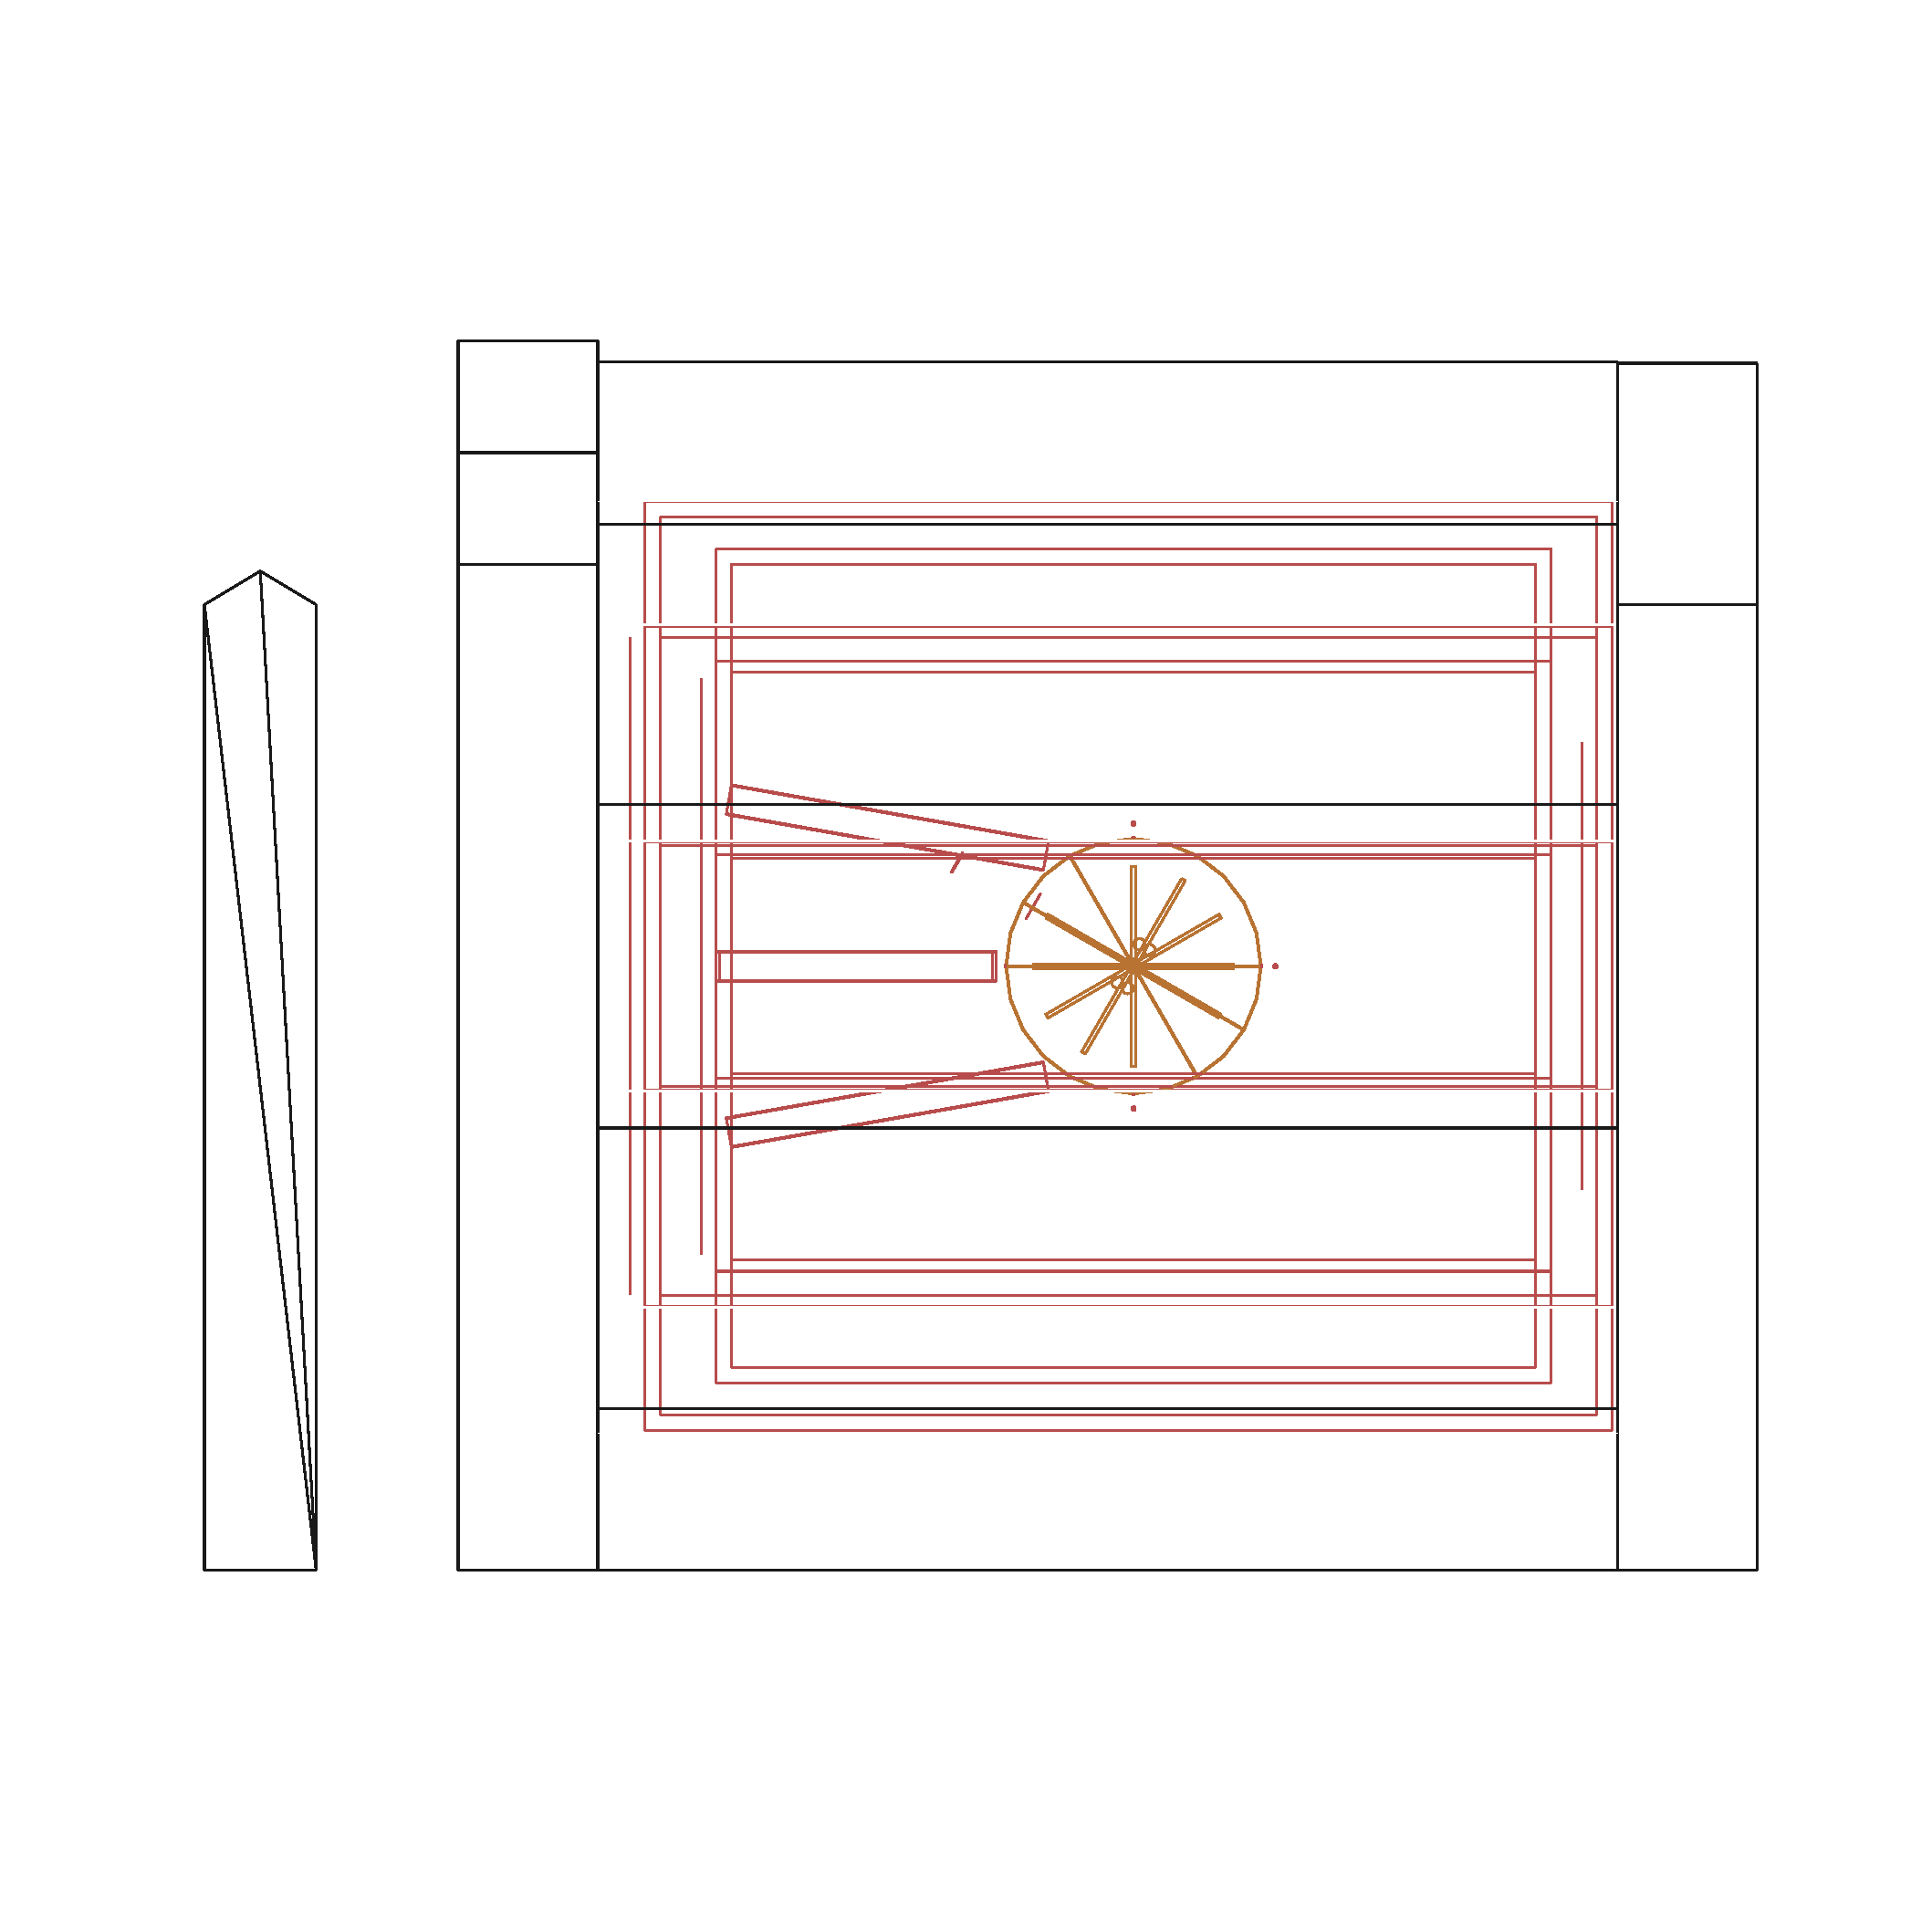
\includegraphics[keepaspectratio=true,width=\textwidth]{OGL_wireframe.eps}
\end{center}
\renewcommand{\baselinestretch}{1}
\small\normalsize
\begin{quote}
\caption{The GEANT simulation includes large-scale features of the EXO-200 detector, including the outer and inner lead wall (black), outer and inner cryostat and TPC legs (red), and the TPC itself (brown).  Components are assembled from simple geometrical shapes, and distant objects are only described coarsely~\cite{MCDocumentRun2a}.}
\label{fig:OGL_wireframevis}
\end{quote}
\end{figure}
\renewcommand{\baselinestretch}{2}
\small\normalsize

\begin{figure}
\begin{center}
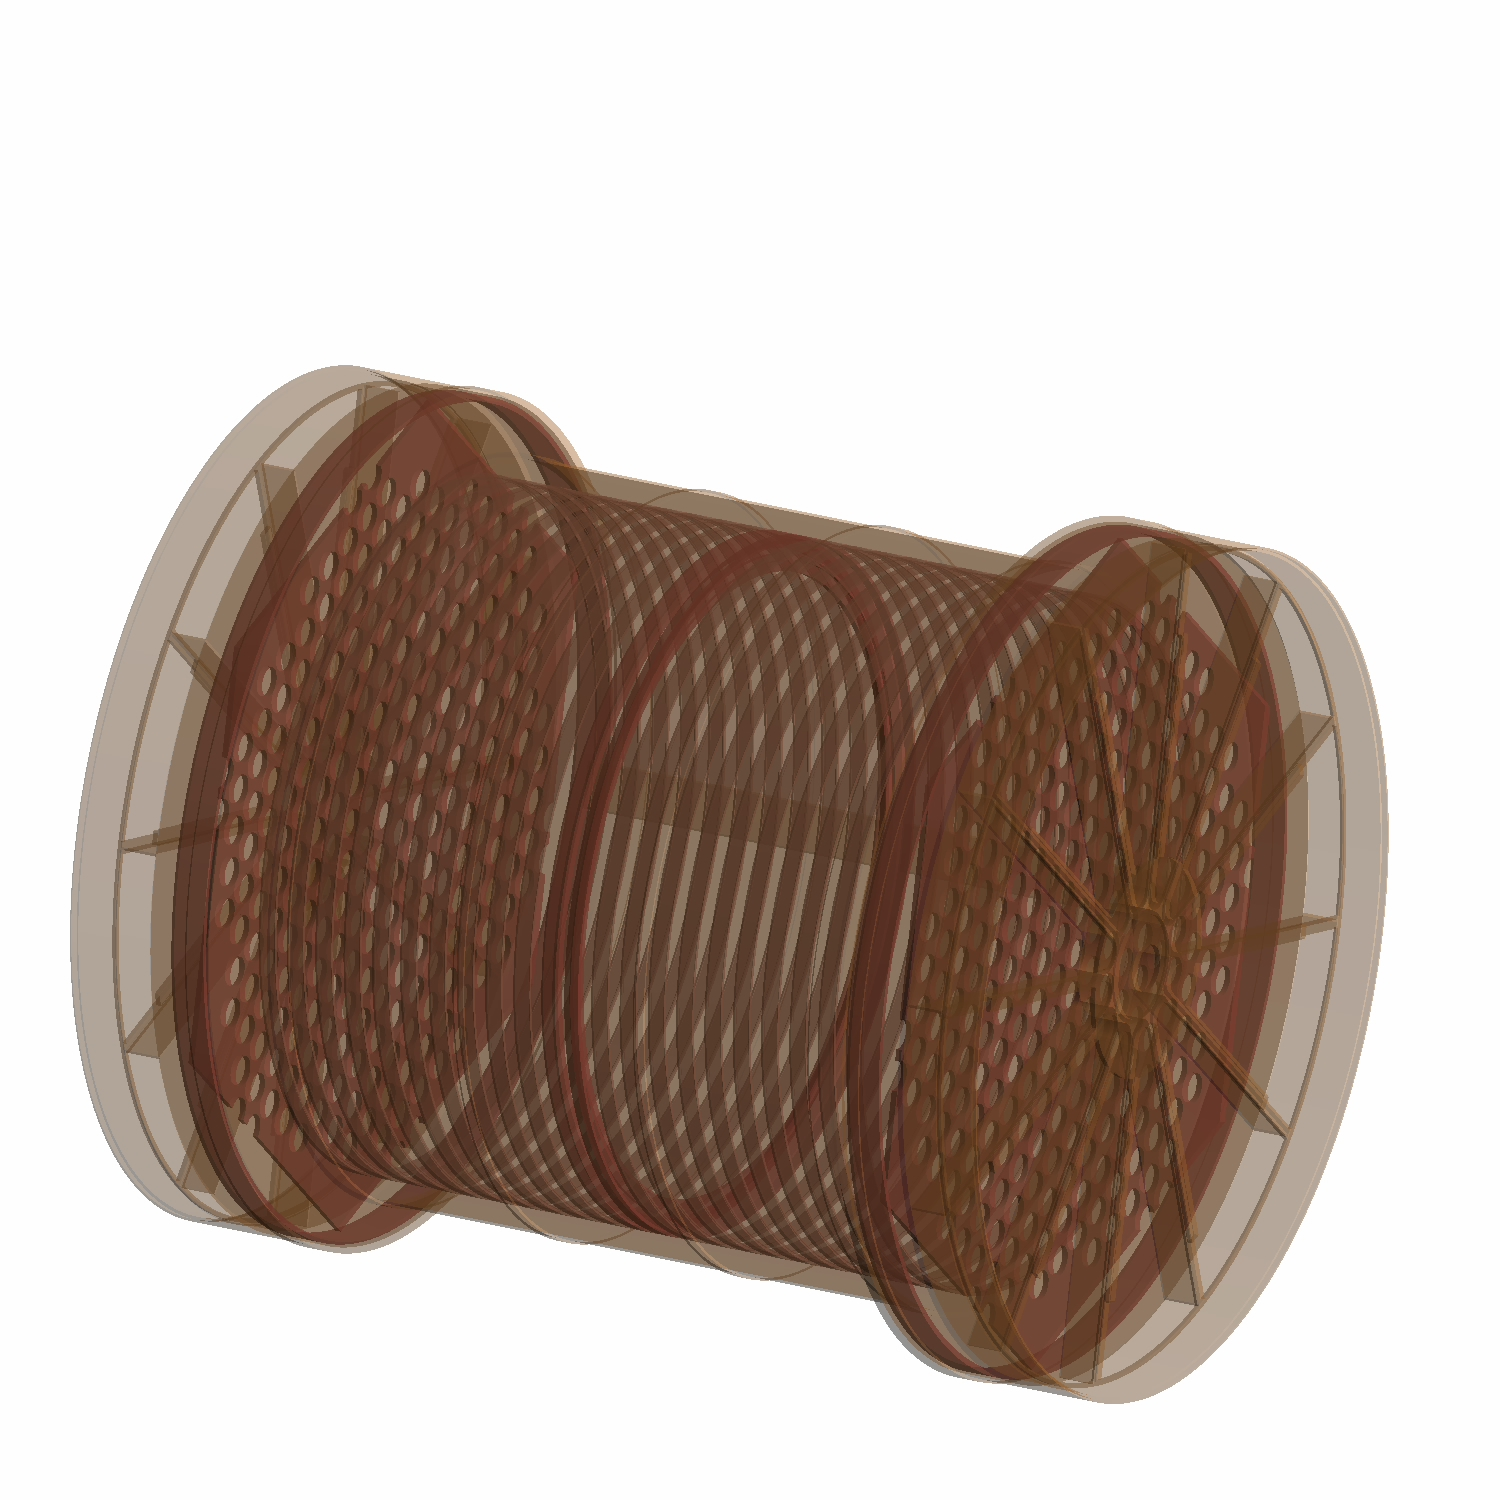
\includegraphics[keepaspectratio=true,width=\textwidth,clip=true,trim=20mm 30mm 35mm 125mm]{TPC_Cu_RayTracer.jpeg}
\end{center}
\renewcommand{\baselinestretch}{1}
\small\normalsize
\begin{quote}
\caption{To ensure computational time is only spent on important details, detector components which are close to the liquid xenon are simulated in GEANT with greater accuracy than distant objects.  The TPC contains the xenon, so it is simulated in detail~\cite{MCDocumentRun2a}.}
\label{fig:RayTracer_TPConly}
\end{quote}
\end{figure}
\renewcommand{\baselinestretch}{2}
\small\normalsize

A model of the EXO-200 detector is simulated in GEANT with a collection of simple geometric volumes which can be composed to form more complicated structures.  Simulation speed decreases as more volumes are generated, and we expect that it is unimportant to simulate details much smaller than the distance between the detail and the liquid xenon.  We attempt to find a balance between accurate modeling of detailed features and simplification of distant features~\cite{MCDocumentRun2a}.  In figure~\ref{fig:OGL_wireframevis} we see the full geometry described in GEANT, where distant objects are constructed from a small number of geometric pieces.  Figure~\ref{fig:RayTracer_TPConly} shows how the TPC is described in GEANT, and we can see the level of detail is much greater.

To simulate particles, GEANT uses a Monte Carlo method.  This means that it models decay processes as a sequence of samples from a probability distribution which are chosen using a pseudorandom number generator.  The energy and direction of the emitted particle, its interaction locations  and quantity of deposited energy, and the formation of secondary particles are all generated randomly as choices from a set of options with known probabilities.  It is possible to override these probability distributions when necessary; for example, EXO-200 uses its own double-beta and forbidden beta decay spectra rather than the defaults provided by GEANT.  Generally, though, the existing options in GEANT are suitable for simulating nuclear and electromagnetic processes~\cite{MCDocumentRun2a}.

Only energy which is deposited in the liquid xenon is observable.  When primary decays are simulated far from the detector, it may be that most of those simulated events deposit no energy in the liquid xenon and are not observable; the simulation continues running until a sufficient number of simulated events deposit energy in the liquid xenon.  This means that sources which are farther from the liquid xenon require significantly more computational time to accumulate a usable number of statistics.  We find that sources outside of the HFE-7000 are subject to $4.5$ attenuation lengths before reaching the liquid xenon, and events reaching the liquid xenon from the inner cryostat can only be simulated at $0.01$ Hz/core by this approach~\cite{MCDocumentRun2a}.

To improve this rate, importance sampling is employed for distant sources.  This approach consists of the following techniques to maximize the impact of limited computational time:~\cite{Dressel:642987,MCDocumentRun2a}
\begin{itemize}
\item Low-energy beta and alpha particles outside of the TPC may be ``killed'', or prematurely eliminated from the simulation based on our knowledge that their attenuation length is quite short.
\item The detector is surrounded by importance sampling ``boundaries'': when a particle passes into a boundary it may be cloned (with a user-selected probability), where the rate of cloning is tracked by a corresponding decrease in particle ``weight.''
\item To avoid biasing the spectrum, it is also necessary to kill particles which pass out of a boundary with the same probability, and increase their weight accordingly.
\end{itemize}
Implicitly, importance sampling simulates the properties of particles reaching the outermost boundary; then draws samples from that distribution and simulates the properties of particles reaching the next boundary; and so forth, amplifying the impact of statistics at each stage.  This also means that statistical errors in the simulated particle distributions at outer boundaries are magnified by this amplification process.  For far backgrounds, though, an approach such as this is essential:  simulation speeds from the inner cryostat are increased from $0.01$ Hz/core to a few Hz/core, and simulations from outside the lead wall which would be wholely infeasible are made possible~\cite{MCDocumentRun2a}.

\begin{figure}
\begin{center}
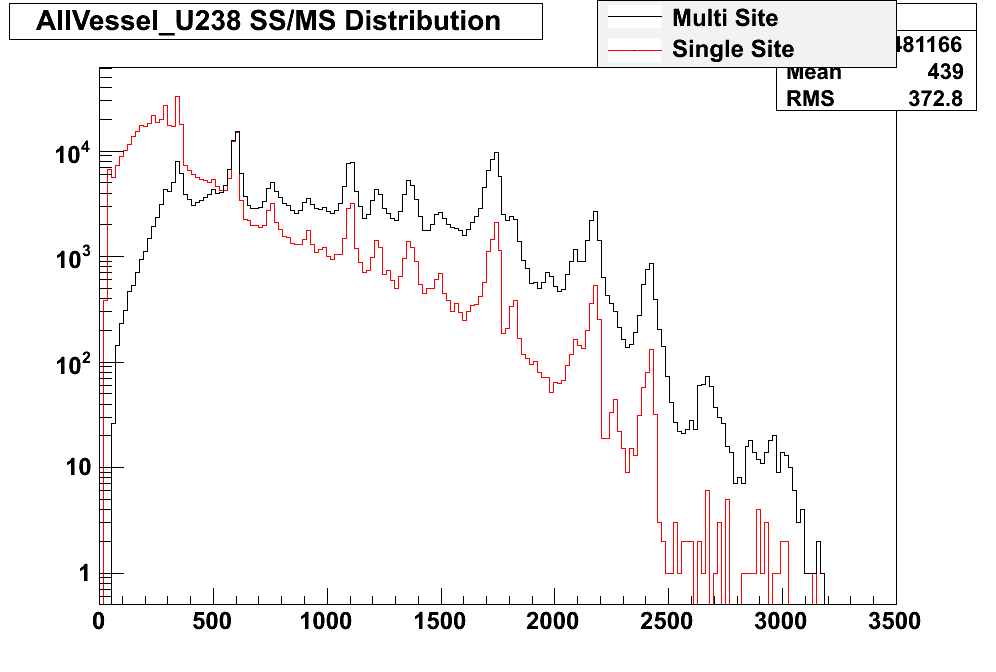
\includegraphics[keepaspectratio=true,width=\textwidth]{AllVessel_U238_single_multi_site_spec.png}
\end{center}
\renewcommand{\baselinestretch}{1}
\small\normalsize
\begin{quote}
\caption{Energy spectra from $^{238}$U in the TPC vessel for single-site (red) and multi-site (black) events.  No energy smearing is performed; peak widths are due to energy loss outside of the liquid xenon~\cite{MCDocumentRun2a}.}
\label{fig:UGeantSpectra}
\end{quote}
\end{figure}
\renewcommand{\baselinestretch}{2}
\small\normalsize

\begin{figure}
\begin{center}
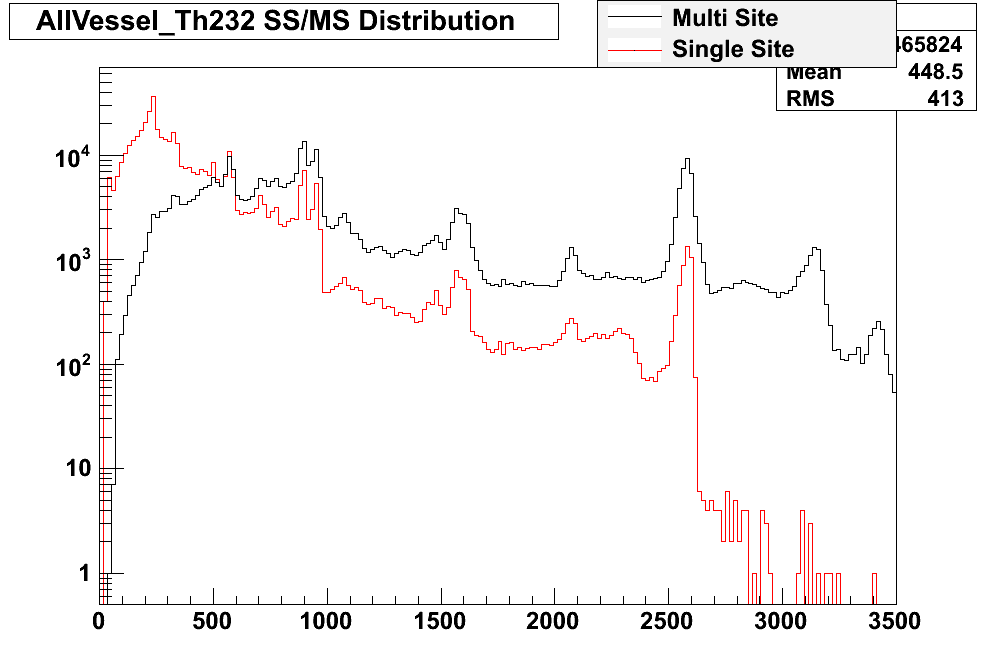
\includegraphics[keepaspectratio=true,width=\textwidth]{AllVessel_Th232_single_multi_site_spec.png}
\end{center}
\renewcommand{\baselinestretch}{1}
\small\normalsize
\begin{quote}
\caption{Energy spectra from $^{232}$Th in the TPC vessel for single-site (red) and multi-site (black) events.  No energy smearing is performed; peak widths are due to energy loss outside of the liquid xenon~\cite{MCDocumentRun2a}.}
\label{fig:ThGeantSpectra}
\end{quote}
\end{figure}
\renewcommand{\baselinestretch}{2}
\small\normalsize

The result of these GEANT simulations is a measurement of the efficiency with which events from various sources reach the liquid xenon, and also of the energy and position spectra of energy deposits from these sources.  Representative spectra of our primary backgrounds, $^{238}$U and $^{232}$Th, are shown in figures~\ref{fig:UGeantSpectra} and \ref{fig:ThGeantSpectra} respectively.

\subsection{Digitization of Waveforms}\label{sec:ResultsDigitization}

After energy deposits are simulated using GEANT, it is necessary to model the conversion of those energy deposits into collected photons and electrons, and then the generation of digitized waveforms resembling the waveforms which are collected in real data.

To generate a scintillation pulse, a purely empirical model is used to estimate the relative pulse magnitudes on the north and south APD planes.  This model only takes into account Z-dependence of the light collection, and does not incorporate the different light yields expected on each individual APD channel.  This model is therefore rather crude, and can only be used as a rough check on the pulse-finding efficiency for scintillation as a function of energy.  Attempts to track optical photons in the TPC have met with only partial success which is insufficient to justify their significant computational cost.  Thus, the EXO simulations are unable to model most aspects of scintillation pulses.  Section~\ref{sec:ResultFitting} will describe the methods used to cope with this aspect of simulation.

\begin{figure}
\begin{center}
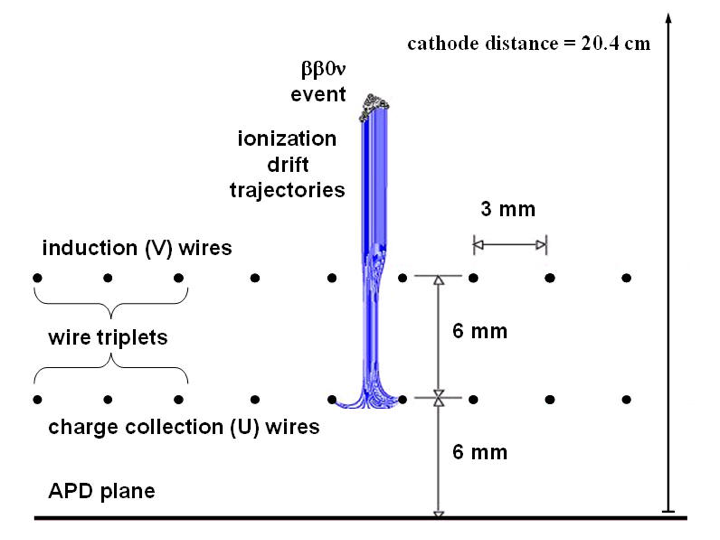
\includegraphics[keepaspectratio=true,width=\textwidth]{ChargeDrift2DModel.png}
\end{center}
\renewcommand{\baselinestretch}{1}
\small\normalsize
\begin{quote}
\caption{The wire planes are modeled in only two dimensions; charge drifts along the field lines, which are arranged to terminate only on the u-wires~\cite{MCDocumentRun2a}.}
\label{fig:TwoDimensionalWireModel}
\end{quote}
\end{figure}
\renewcommand{\baselinestretch}{2}
\small\normalsize

Simulation of charge pulses is better-understood.  The detector's electric field is modeled in a two-dimensional geometry illustrated in figure~\ref{fig:TwoDimensionalWireModel} where, rather than one-dimensional wires arranged in two-dimensional planes, we have wire ``points'' at fixed voltage which are grouped in a one-dimensional pattern.  The v-wires are treated as stacked directly on top of the u-wires; it is impossible in two dimensions to model the true orientation of the v-wires which is rotated relative to the u-wires, but this has generally proven to be a minor detail for us.  Only one TPC half is modeled because of the approximate mirror symmetry of the detector across the cathode.  We assume that the two-dimensional geometry is periodic along the direction of the wire ``plane'', which permits us to always locate drifting charge above the central wire.  Only a few wires to either side of the center are simulated because each wire acts as a shield between wires to its left and right, so the electrostatic effect of any one wire will be not extend beyond a few wire spacings~\cite{MCDocumentRun2a}.

Electrostatic effects are simulated using the ANSYS Maxwell field simulator.  To simulate the electric fields in the detector, wires are treated as circles with a radius matching the approximate radii of the physical wires, with a constant voltage on their surfaces.  The APD plane and cathode plane are treated as constant-voltage boundaries, and a periodic boundary condition is established on the two remaining boundaries of the model geometry.

These electric fields can be used to trace the paths followed by charge deposits in the detector.  Charge deposits are drifted in small steps based on the direction of the electric field.  The speed of drift is taken from external measurements rather than from the magnitude of the electric field; in most of the bulk of xenon, the electric field and drift velocity are treated as constant, but near the u-wire plane the drift velocity is increased slightly to account for higher electric fields experienced in that region of the detector.  Charge attenuation due to finite purity can be modeled at this step, but generally is treated as infinite here; charge diffusion effects are ignored.

\begin{figure}
\begin{center}
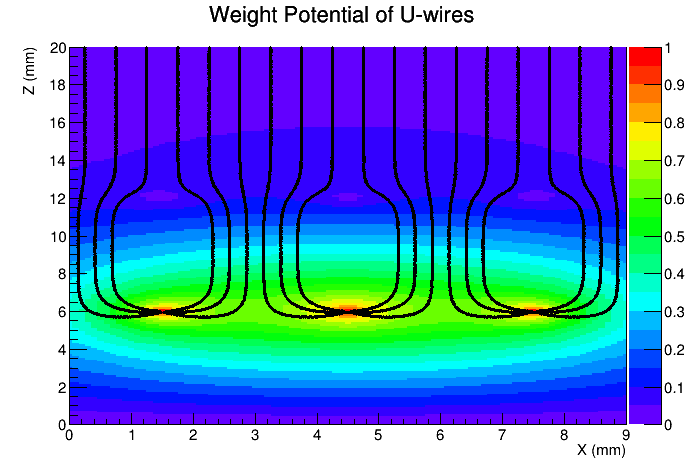
\includegraphics[keepaspectratio=true,width=\textwidth]{WeightPotContoursU_WithE.png}
\end{center}
\renewcommand{\baselinestretch}{1}
\small\normalsize
\begin{quote}
\caption{Weight potential of a u-wire channel consisting of three ganged wires.  Electric field lines are superimposed~\cite{MCDocumentRun2a}.}
\label{fig:UWireWeightPotential}
\end{quote}
\end{figure}
\renewcommand{\baselinestretch}{2}
\small\normalsize

\begin{figure}
\begin{center}
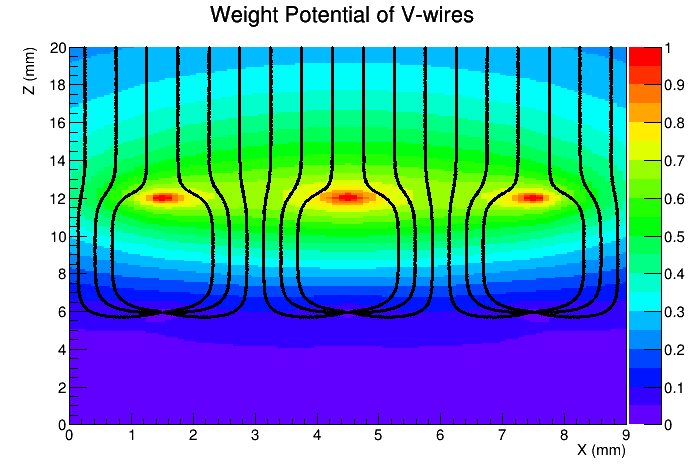
\includegraphics[keepaspectratio=true,width=\textwidth]{WeightPotContoursV_WithE.png}
\end{center}
\renewcommand{\baselinestretch}{1}
\small\normalsize
\begin{quote}
\caption{Weight potential of a v-wire channel consisting of three ganged wires.  Electric field lines are superimposed~\cite{MCDocumentRun2a}.}
\label{fig:VWireWeightPotential}
\end{quote}
\end{figure}
\renewcommand{\baselinestretch}{2}
\small\normalsize

We have discussed in section~\ref{sec:DetectorReadout} that charge is induced on the u-wires and v-wires; this means that we must record the amount of charge induced at each step along the drift path of the charge deposit.  This is done based on the Shockley-Ramo Theorem, which states that the change in induced charge $\delta q_i$ on an electrode $i$ is equal to:
\begin{equation}
\delta q_i = Q \delta W_i,
\end{equation}
where $Q$ is the total drifting charge and $W_i$ is the weighting potential of electrode $i$, defined as the potential which would be induced in our geometry if the potential on electrode $i$ were set to one and the potential on all other boundaries were set to zero~\cite{ShockleyPaper,1686997}.  Figures~\ref{fig:UWireWeightPotential} and~\ref{fig:VWireWeightPotential} illustrate the weighting potentials of a u-wire and v-wire channel, respectively.

Finally, the functions of integrated charge versus time must be converted to shaped digitized waveforms, and noise must be added.  The shaping and gain amplification is performed to match the electronics described in section~\ref{sec:DetectorReadout}.  To ensure accurate time shaping, the functions are all sampled at a bandwidth of $10$ MHz, and then downsampled after shaping to the nominal $1$ MHz.  Digitization is performed by converting voltages into units of ADC counts, then truncating to an integer value.  To model saturation effects, this number is pulled into the integer range $[0, 4096)$.

\begin{figure}
\begin{center}
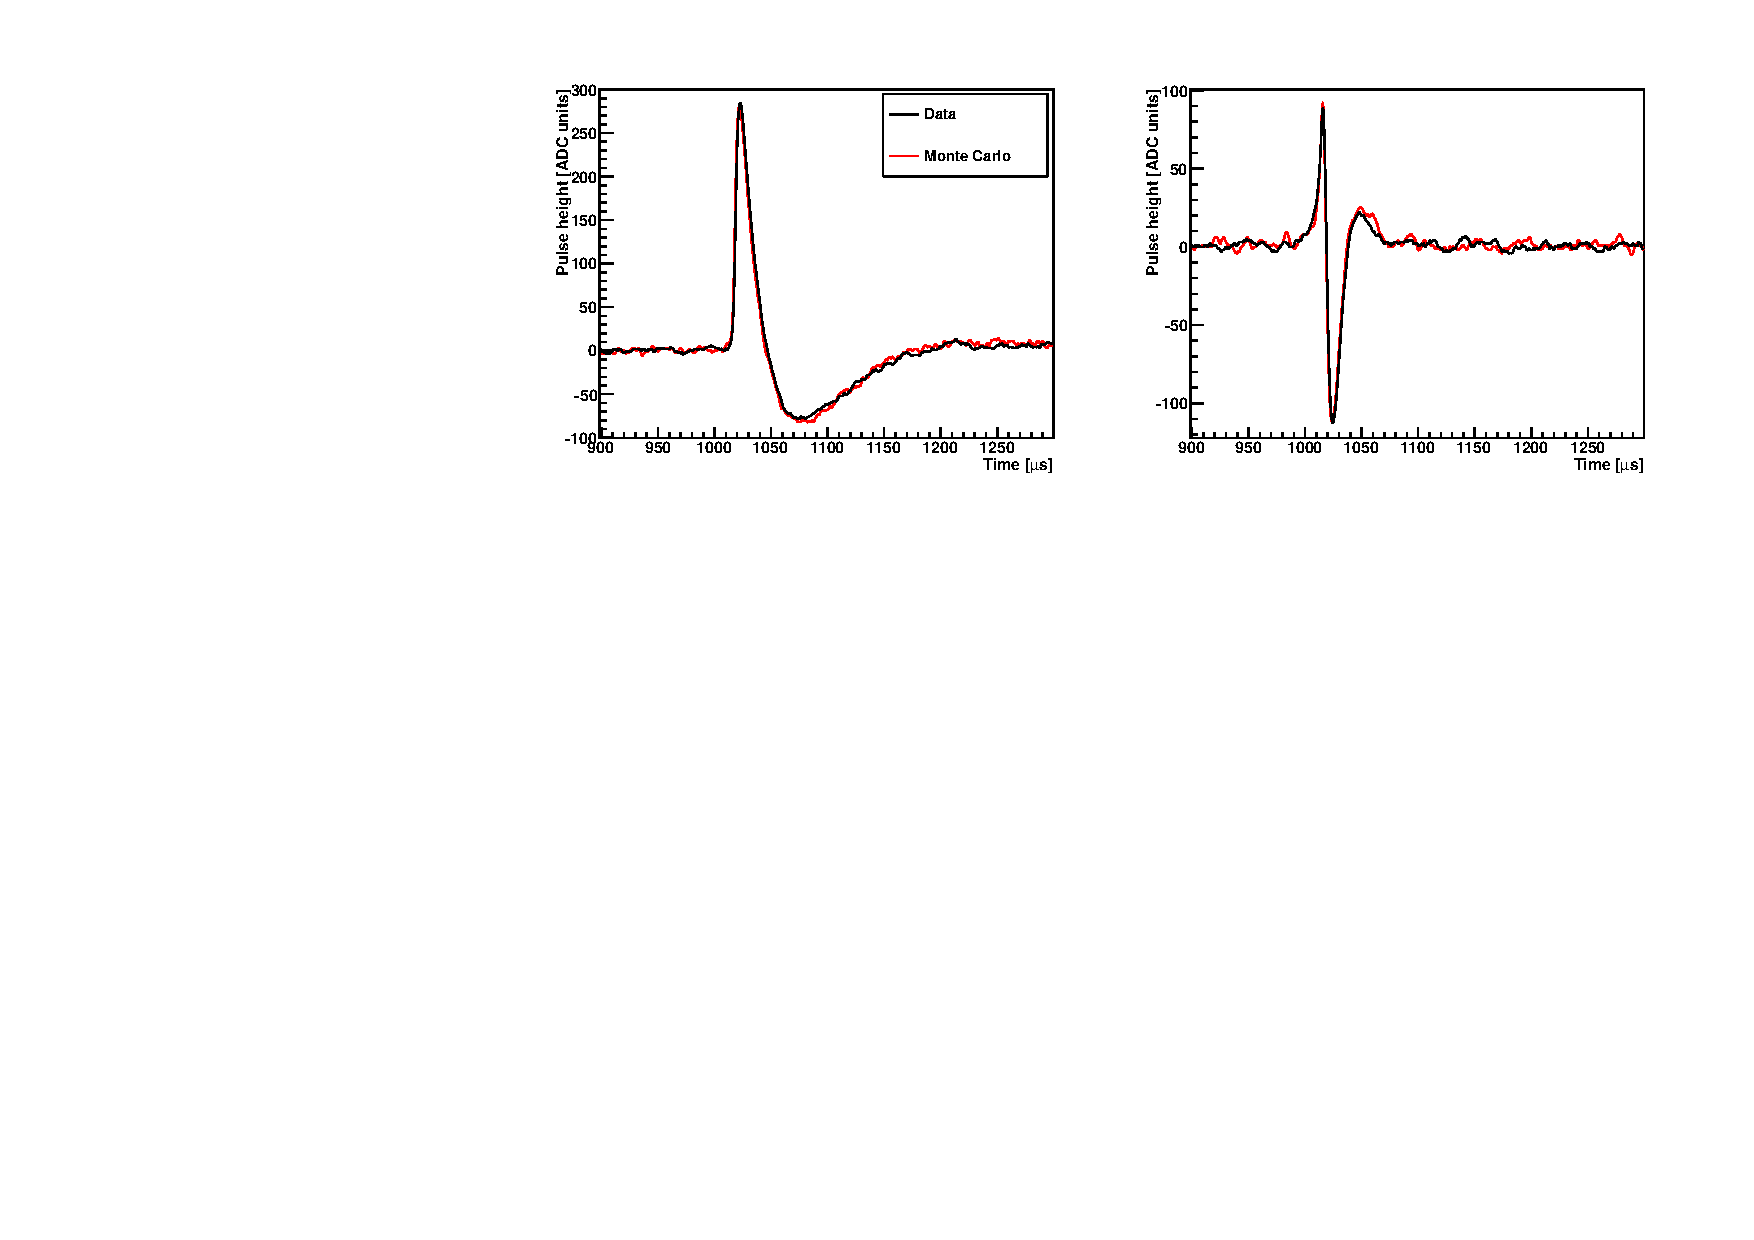
\includegraphics[keepaspectratio=true,width=\textwidth]{pulse_comp.pdf}
\end{center}
\renewcommand{\baselinestretch}{1}
\small\normalsize
\begin{quote}
\caption{Comparison between simulated and observed waveforms on a u-wire (left) and v-wire (right) from $^{228}$Th sources.  The events are chosen to have similar energies so that the magnitudes match~\cite{MCDocumentRun2a}.}
\label{fig:MCPulseComparison}
\end{quote}
\end{figure}
\renewcommand{\baselinestretch}{2}
\small\normalsize

We have the ability to add electronic noise to the pulses by extracting a set of representative noise waveforms from real data.  These are taken from a large number of solicited triggers which have been checked for the absence of a coincident event.  To increase the number of noise waveforms available, the noise waveforms sampled from the detector are spliced together, and simulated events may draw their noise from any subrange of the spliced-together noise waveform.  This method provides our most accurate noise model because it can include all noise frequency peaks and channel correlations without requiring a full understanding of those features.

However, current analyses do not employ this method; instead, we simulate noise which is white (has a flat Fourier spectrum) before shaping, and then shaped to have a spectrum which roughly resembles the one observed in the detector.  Figure~\ref{fig:MCPulseComparison} compares waveforms observed from a sample event in data and simulation, and demonstrates that at high energies excellent agreement is achieved~\cite{MCDocumentRun2a}.

\begin{figure}
\begin{center}
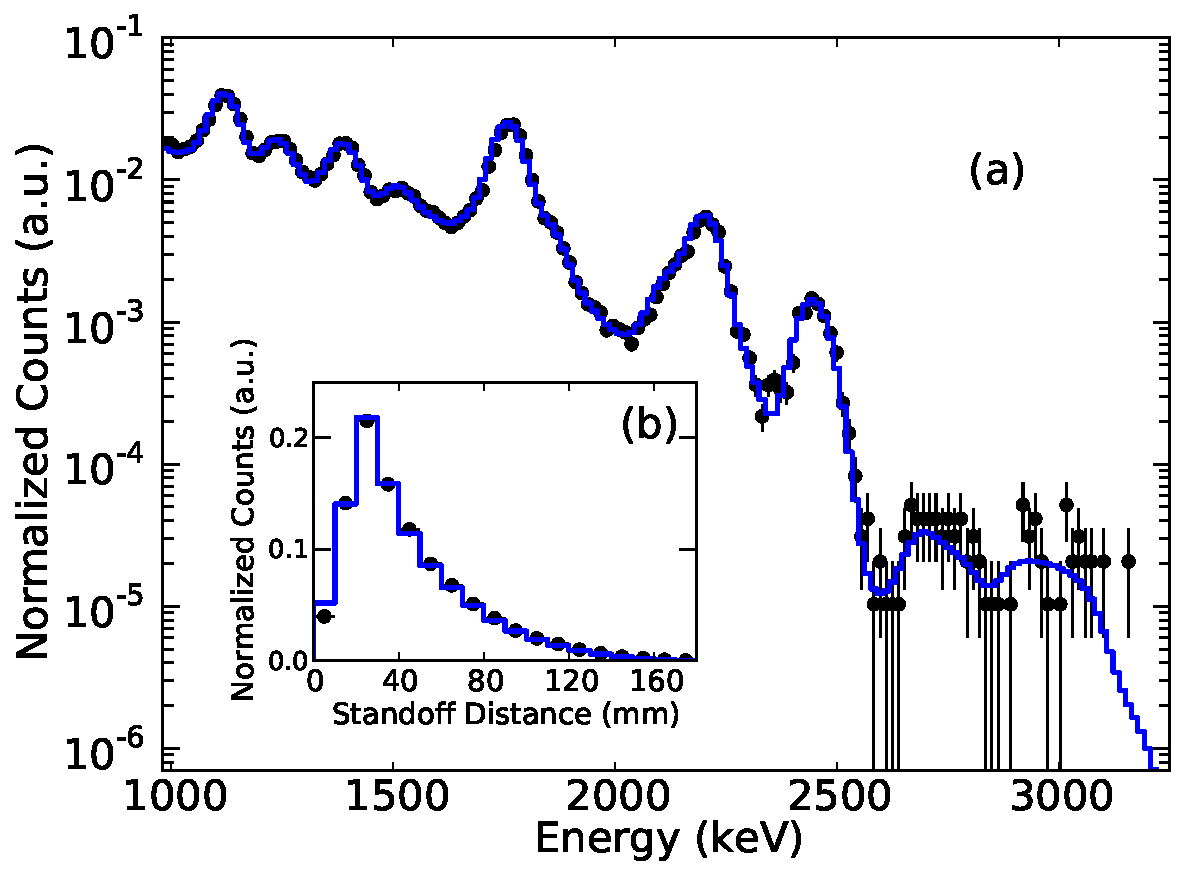
\includegraphics[keepaspectratio=true,width=\textwidth]{SS_Ra226_Campaign7.pdf}
\end{center}
\renewcommand{\baselinestretch}{1}
\small\normalsize
\begin{quote}
\caption{Comparison between simulated and observed energy spectra (a) and standoff distance (b) in single-site $^{226}$Ra events from a source located at position S5~\cite{NewEXObb0nPaper_2014}.}
\label{fig:RaSourceMCComparison}
\end{quote}
\end{figure}
\renewcommand{\baselinestretch}{2}
\small\normalsize

In this way, we are able to generate simulated data which in most respects resembles real data collected from the detector.  The EXO-200 simulation has shown remarkable agreement with the detector in the properties of energy and cluster location, as illustrated in figure~\ref{fig:RaSourceMCComparison}.  A significant effort has been made to achieve excellent agreement between simulation and data, and the result is that we can claim a strong understanding of the behavior of the EXO-200 detector.

\section{Cluster Reconstruction}\label{sec:ResultReconstruction}

The first stage of data processing involves locating candidate pulses in its waveforms and fitting for the magnitude and time of any candidate pulses which are found.  The methods of accomplishing this are described in sections~\ref{sec:ReconPulseFinding} and~\ref{sec:ReconPulseFitting}.  We will complete our description of cluster reconstruction with a brief explanation of the approach to the clustering of waveform pulses into three-dimensional clusters in section~\ref{sec:ReconClustering}.

\subsection{Pulse Finding}\label{sec:ReconPulseFinding}

Pulse-finding proceeds in two steps.  First, on u-wire, v-wire, and summed APD waveforms a matched filter is applied to do a preliminary search on all channels.  Then, a secondary search is performed on the u-wire waveforms to improve sensitivity to multiple pulses near in time.

The matched filter algorithm was first described by D.O. North in 1943~\cite{MatchedFilterPaper}.  It attempts to decide between the null hypothesis that a waveform $X[\tau]$ consists of only noise and an alternative hypotheses that the waveform contains a pulse and noise:
\begin{equation}\begin{cases}
H_0: & X[\tau] = n[\tau]\\
H_1: & X[\tau] = s[\tau] + n[\tau].
\end{cases}\end{equation}
To discriminate between these hypotheses optimally, we search for a linear functional $L_0$ which will act on $X[\tau]$ and maximize the expected signal-to-noise ratio,
\begin{equation}
SNR = \frac{\left(L_0\left\{s[\tau]\right\}\right)^2} {\left<\left(L_0\left\{n[\tau]\right\}\right)^2\right>}.
\end{equation}
In other words, if a waveform is composed of only noise, the functional should result in a small value; however, if the waveform contains a pulse then the functional should result in a large value.

We omit the derivation, which is a standard result, and simply state that the linear functional which maximizes the expected signal-to-noise ratio can be expressed as:~\cite{MatchedFilterPaper}
\begin{equation}
L_0\left\{X[\tau]\right\} = \mathcal{F}^{-1}\left\{ \frac{\mathcal{F}\left\{X\right\}[k] \mathcal{F}\left\{s\right\}^{*}[k]}{\left<\mathcal{F}\left\{N\right\}[k]\mathcal{F}\left\{N\right\}^{*}[k]\right>}\right\}[0],
\end{equation}
where $\mathcal{F}$ represents the Fourier transform.  This expression has an added benefit that if instead we'd like to test the hypothesis that the translated pulse $s[\tau - \Delta]$ is contained in the waveform, substitution lets us show that we can do so with the related test statistic:
\begin{equation}
L_\Delta\left\{X[\tau]\right\} = \mathcal{F}^{-1}\left\{ \frac{\mathcal{F}\left\{X\right\}[k] \mathcal{F}\left\{s\right\}^{*}[k]}{\left<\mathcal{F}\left\{N\right\}[k]\mathcal{F}\left\{N\right\}^{*}[k]\right>}\right\}[\Delta].
\end{equation}
Finally, we can define a test statistic $T$ for the waveform $X[\tau]$ to have a pulse anywhere with:
\begin{equation}
T = \max_{\Delta} L_\Delta\left\{X[\tau]\right\}.
\end{equation}
The values $L_\Delta$ for all $\Delta$ can be computed efficiently using the fast Fourier transform.  The time of the pulse is guessed as the value of $\Delta$ which led to the maximum of $L_\Delta\left\{X[\tau]\right\}$.

\begin{figure}
\begin{center}
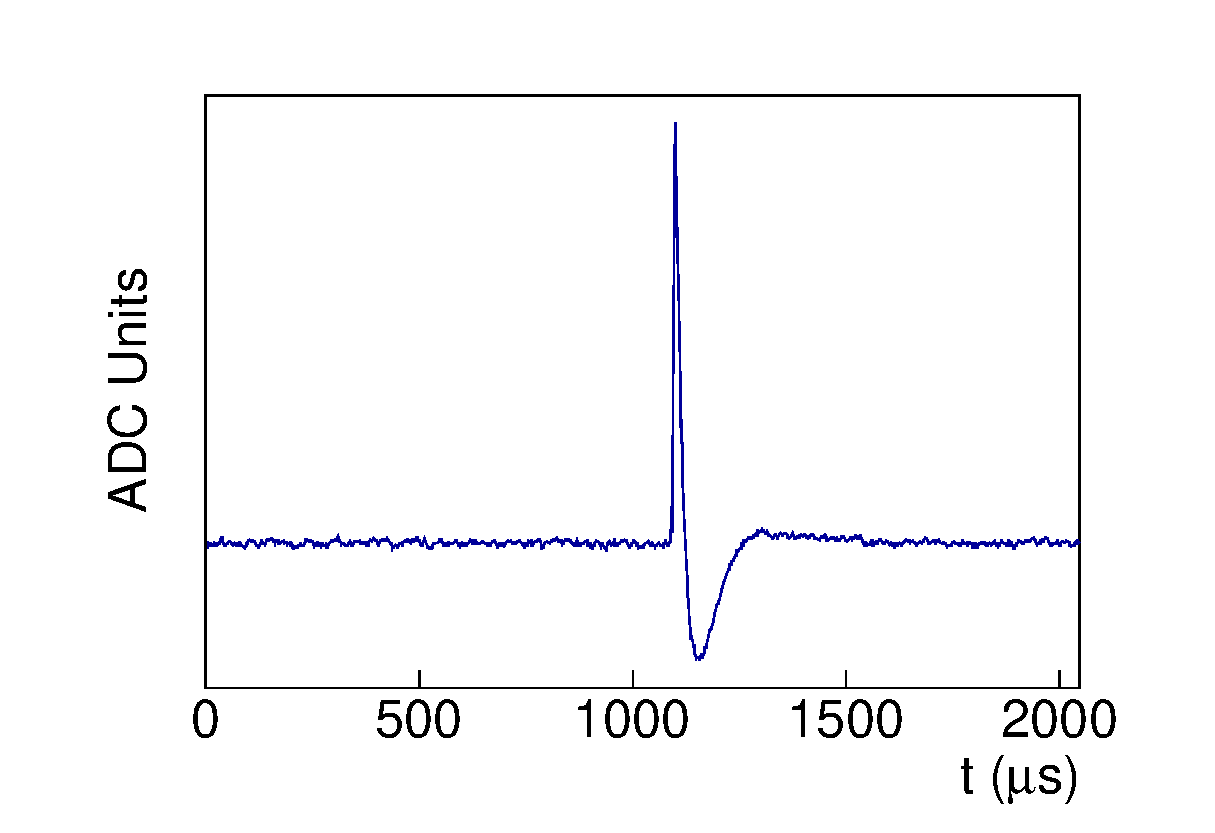
\includegraphics[keepaspectratio=true,width=.49\textwidth]{MFExamp_Raw.eps}
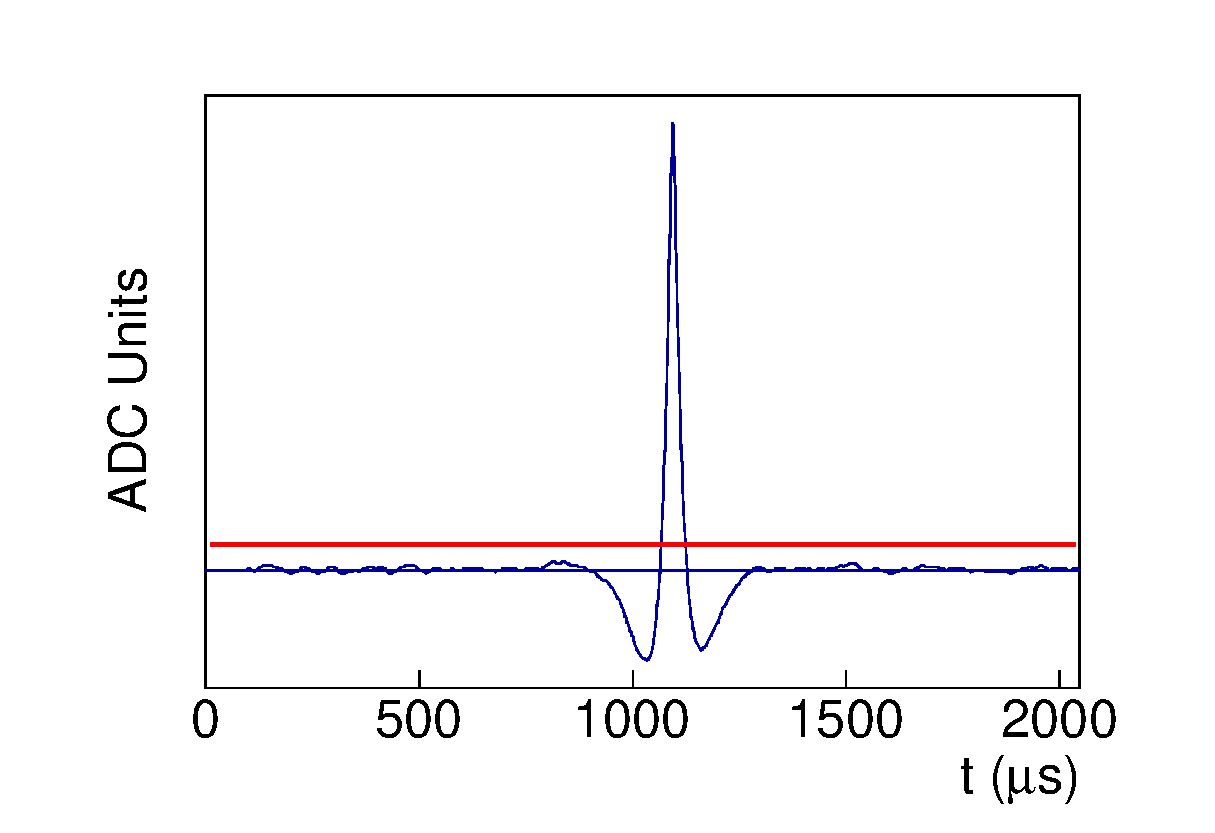
\includegraphics[keepaspectratio=true,width=.49\textwidth]{MFExamp_Applied.eps}
\end{center}
\renewcommand{\baselinestretch}{1}
\small\normalsize
\begin{quote}
\caption{A u-wire waveform (left) and the output from operation of the matched filter (right).  The red line on the right indicates our filtered pulse threshold; the matched filter output exceeds the threshold, so this waveform is determined to contain a pulse~\cite{ReconstructionDocument}.}
\label{fig:MatchedFilterApplication}
\end{quote}
\end{figure}
\renewcommand{\baselinestretch}{2}
\small\normalsize

The first phase of pulse-finding performs a search using the matched filter on:
\begin{itemize}
\item All u-wire channels.
\item All v-wire channels.
\item The sum of all APD channels in the North plane.
\item The sum of all APD channels in the South plane.
\end{itemize}
An example application of the matched filter to a u-wire waveform is shown in figure~\ref{fig:MatchedFilterApplication}.

\begin{figure}
\begin{center}
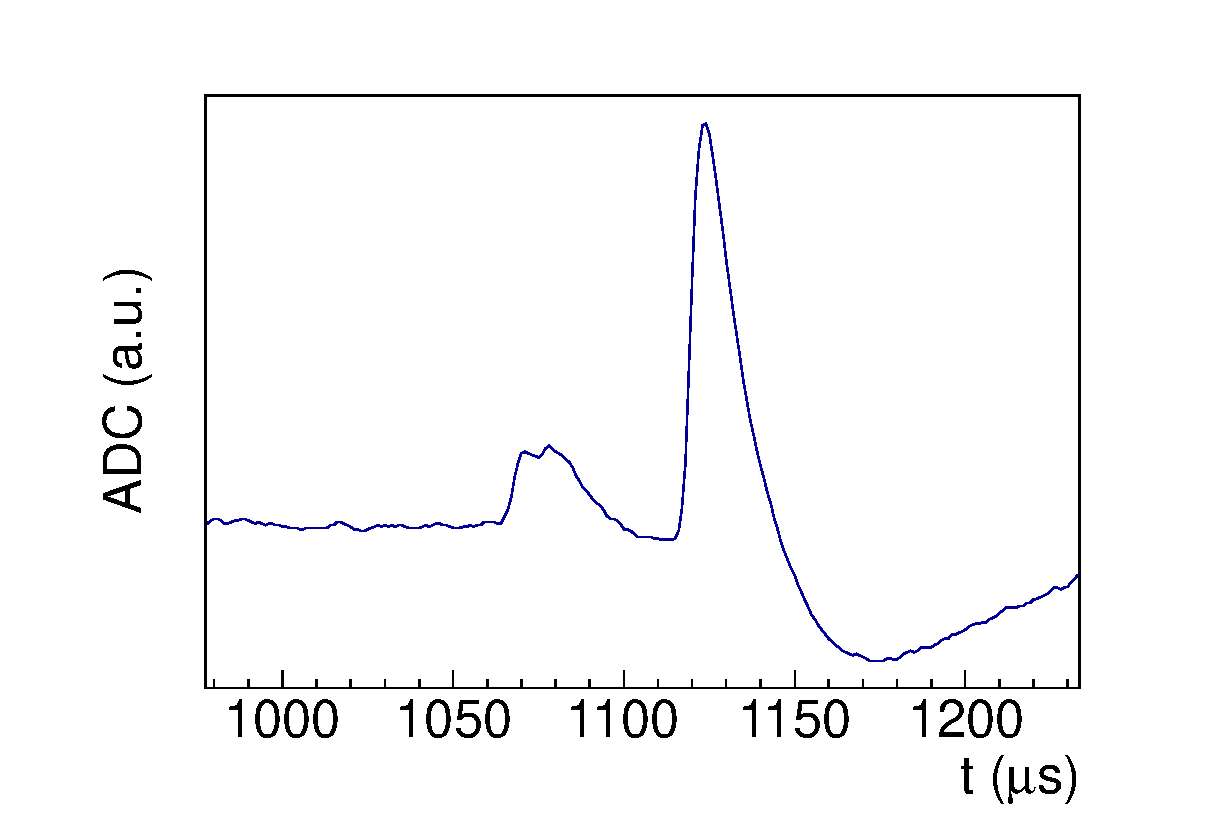
\includegraphics[keepaspectratio=true,width=.49\textwidth]{MSF_Raw.eps}
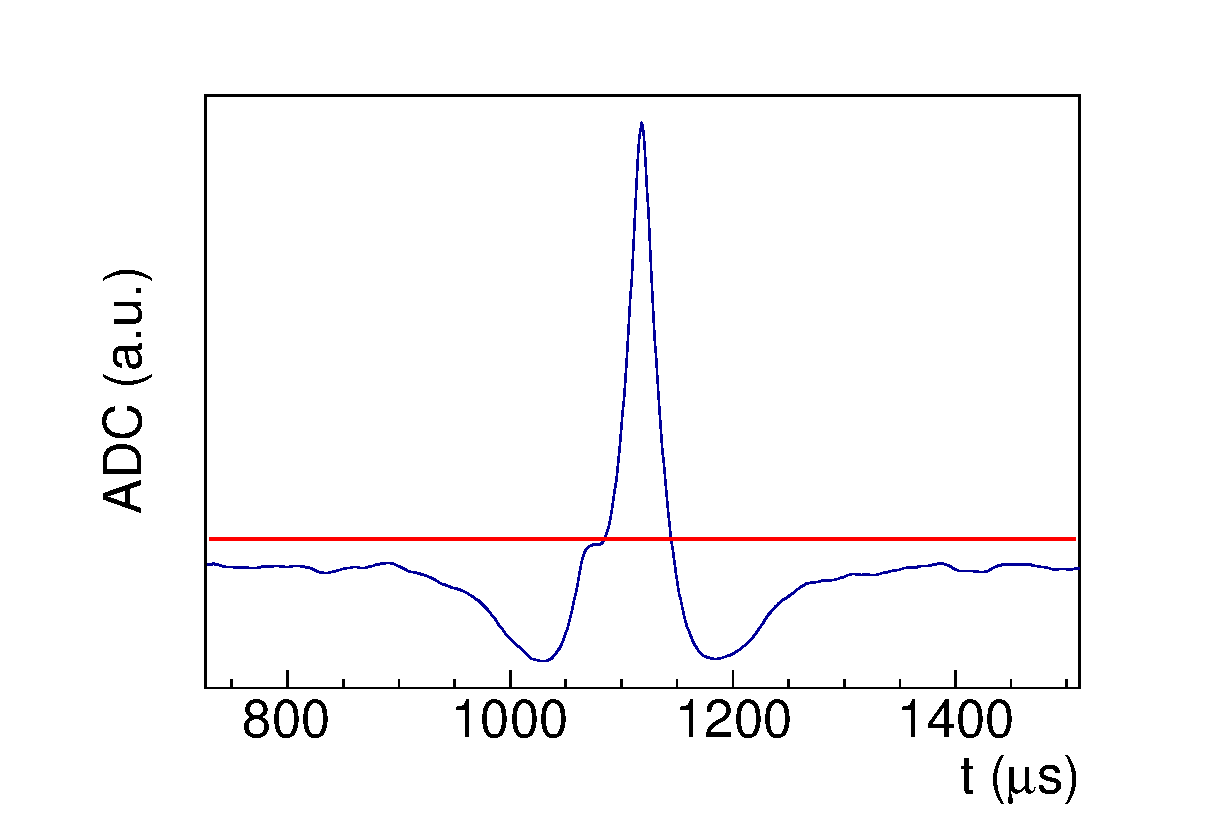
\includegraphics[keepaspectratio=true,width=.49\textwidth]{MSF_MatchedFilter.eps}
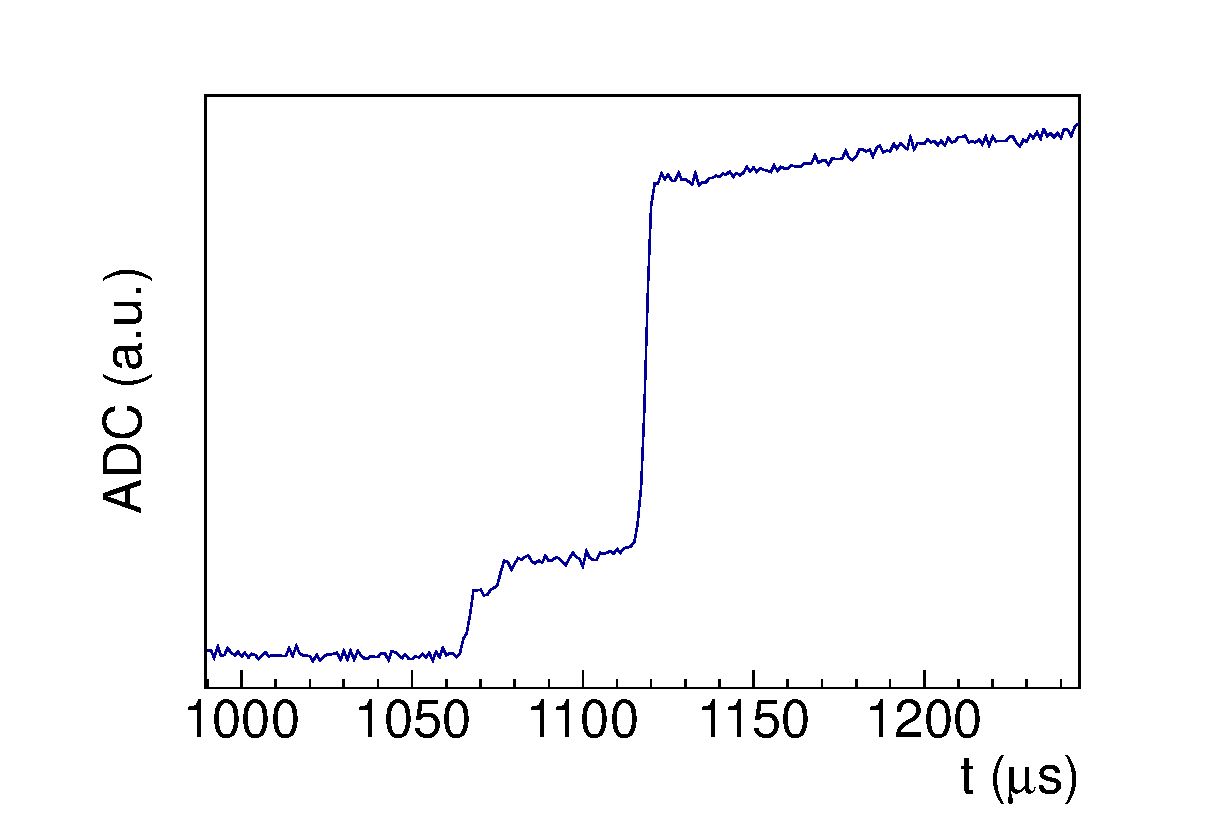
\includegraphics[keepaspectratio=true,width=.49\textwidth]{MSF_Unshaped.eps}
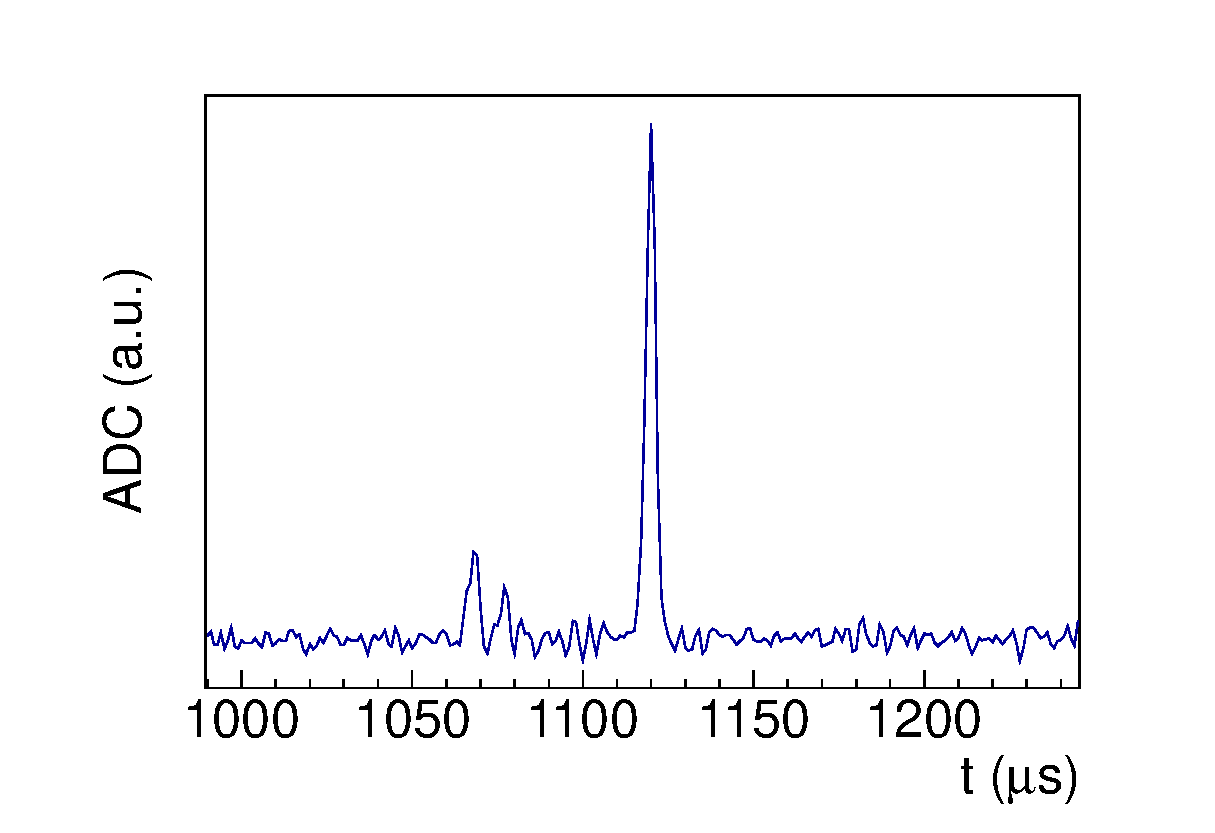
\includegraphics[keepaspectratio=true,width=.49\textwidth]{MSF_Reshaped.eps}
\end{center}
\renewcommand{\baselinestretch}{1}
\small\normalsize
\begin{quote}
\caption{A u-wire waveform composed of two pulses near in time is shown (top left); the matched filter (top right) correctly detects the presence of a pulse, but does not detect the presence of two distinct pulses.  At bottom left, the waveform is unshaped; at bottom right the waveform is reshaped with shorter differentiation times, leading to easier detection~\cite{ReconstructionDocument}.}
\label{fig:MultipleSignalFinderApplication}
\end{quote}
\end{figure}
\renewcommand{\baselinestretch}{2}
\small\normalsize

The matched filter has proven to be an excellent metric for deciding whether a waveform has a pulse on it or not.  However, it is not as effective at distinguishing between the cases where one or multiple pulses occur on a waveform.  We would particularly like to be able to classify u-wire waveforms by the number of distinct pulses they contain because this can help us distinguish between single-site and multi-site events, which can reduce our background as described in section~\ref{sec:DetectorActiveBackgroundRejection}.  The matched filter output function is designed to have a tall peak in the presence of a pulse, but it may also be a broad peak which is difficult to resolve as the sum of two distinct pulse contributions.

To improve sensitivity to multiple pulses in u-wire waveforms, a second pass is performed on u-wire channels using a multiple-signal finder.  This scheme consists of first unshaping the waveform offline to remove the effect of the shapers, and then reshaping the waveform using shorter differentiation times than the hardware shapers apply.  This is a type of high-pass filter; in a multiple-pulse waveform, it can have the effect of damping the first pulse faster to reduce its overlap in time with the second pulse.  It is then possible to search for pulses using a simple threshold which is not as sensitive to small pulses as the matched filter, but is capable of detecting additional pulses to complement the matched filter.  This process is illustrated in figure~\ref{fig:MultipleSignalFinderApplication}, and is the last procedure for finding pulses~\cite{ReconstructionDocument}.

\subsection{Pulse Fitting}\label{sec:ReconPulseFitting}

After finding pulses, it is necessary to perform a fit to the expected pulse shape.  Fits are performed allowing both the pulse magnitude and time to float freely, where only the initial guesses for these parameters come from the finding step.  The metric for fits is a simple chi-square between waveform data and the expected pulse shape, where error on each point is estimated by the root-mean-square noise of the channel.

\begin{figure}
\begin{center}
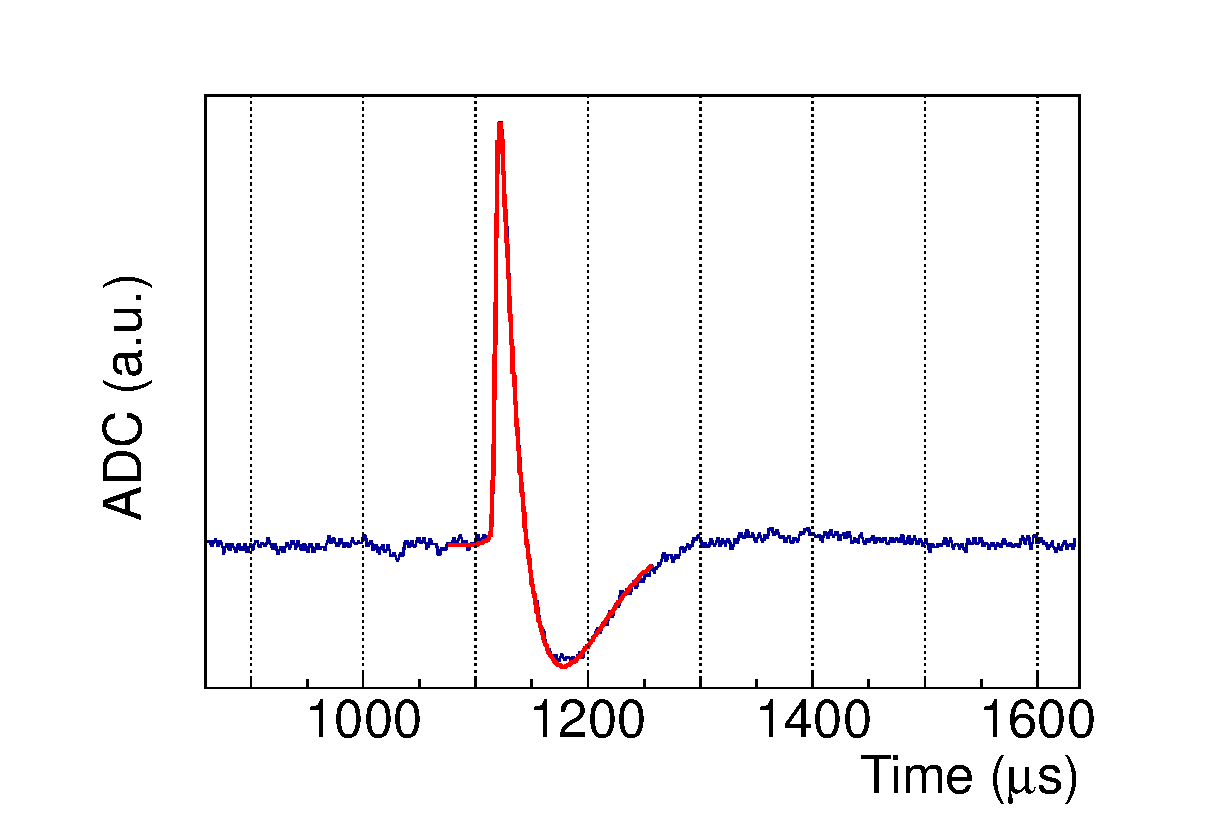
\includegraphics[keepaspectratio=true,width=.49\textwidth]{U_Wire_Fit.eps}
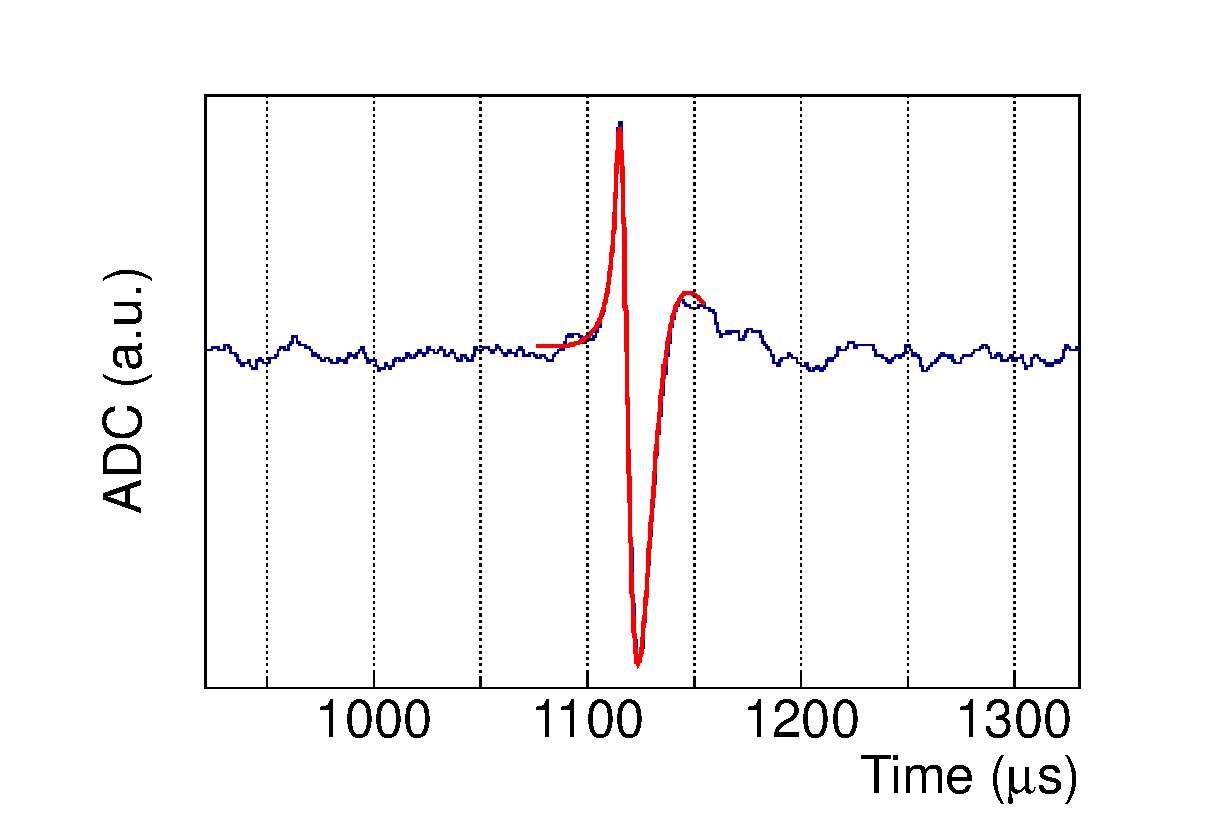
\includegraphics[keepaspectratio=true,width=.49\textwidth]{V_Wire_Fit.eps}
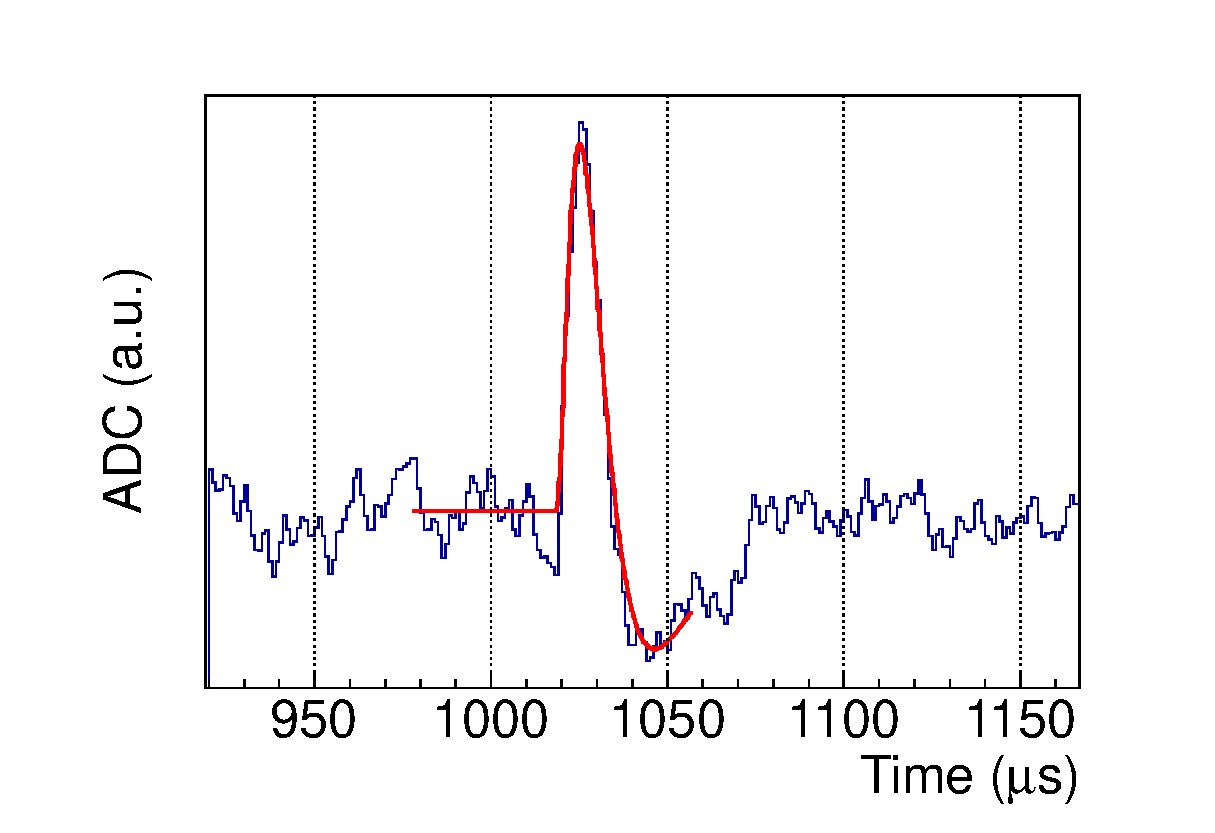
\includegraphics[keepaspectratio=true,width=.49\textwidth]{APD_Sum_Fit.eps}
\end{center}
\renewcommand{\baselinestretch}{1}
\small\normalsize
\begin{quote}
\caption{Fits to data for a u-wire (top left), v-wire (top right), and summed-APD waveform (bottom).  The red model line indicates the time extent of the fit window~\cite{ReconstructionDocument}.}
\label{fig:ReconExampleFits}
\end{quote}
\end{figure}
\renewcommand{\baselinestretch}{2}
\small\normalsize

To minimize the impact of pulse templates whose shape may not perfectly reflect the shaping times in hardware, and also to reduce the effect which waveform noise may have on our fit, we do not fit the entire waveform to our pulse model.  Instead, we use only an $80 \mu$s fit window in the case of v-wires and APDs, and a $180 \mu$s fit window in the case of u-wires.  The fit windows are illustrated with example events in figure~\ref{fig:ReconExampleFits}.

As pulse times and magnitudes are extracted, it may be discovered at this phase of processing that two pulses on the same waveform which were separately reported by the finding phase are extremely close together in time.  In this case, we can generally conclude that the finding phase inadvertently reported the same pulse multiple times; the multiple candidate pulses should then be merged together, and the waveform refit.  The specific criteria for merging or removing candidate pulses are:~\cite{ReconstructionDocument}
\begin{itemize}
\item If two pulses occur within 10 $\mu$s of each other and one pulse has a fit magnitude error of at least 15 ADC counts, the two pulses are merged.
\item If any pulse has a magnitude to magnitude-error ratio of less than 6.0 for u-wires, 5.0 for summed APD waveforms, or 3.0 for v-wires, then the smallest such pulse is removed.
\item If any pulse has a magnitude of less than 5 ADC counts, then the smallest such pulse is removed.
\end{itemize}
Each time a single pulse is removed or a pair of pulses is merged, the fit is re-run and we search again for any pulses warranting removal.  In this way, we attempt to ensure at the pulse-fitting stage that only appropriate fit results are retained.

\subsection{Clustering Pulses into Deposit Sites}\label{sec:ReconClustering}

The result of pulse finding and fitting is a list of pulse magnitudes and times for each channel.  It remains for reconstruction to combine this information into three-dimensional clusters, where each cluster should have a three-dimensional position, time, and estimates for charge and light pulse magnitudes.

We begin by bundling groups of similar u-wire, v-wire, and APD pulses.  Multiple u-wire pulses may be bundled together when they occur on neighboring channels close together in time.  This may represent a cluster which occurred halfway between two u-wire channels and was split, with some charge being collected by each u-wire channel; it may also represent a combination of charge being collected on one channel and an induced charge pulse on a nearby u-wire channel due to the proximity of the charge drift path to that neighboring channel.  V-wire pulses are bundled together based on a combination of pulse magnitude and time to account for the observation that the passage of a single charge cloud will induce pulses on many nearby v-wires.  APD pulses are bundled based on time only, particularly to ensure that when a pulse is observed on both the North and South APD planes, the pulses are interpreted as originating from the same event in the detector.

We then attempt to join u-wire pulse bundles and APD pulse bundles into two-dimensional charge clusters, identified by their U-Z positions and the time of the energy deposit.  The algorithm to do this is simple: for each u-wire pulse bundle, we join it with the most recent APD pulse bundle in the event.  The maximum difference in time is the maximum drift time of charge clusters in the detector, $116 \mu$s.  To allow for fit errors in the time parameters of the APD and u-wire pulses, an additional $3 \mu$s allowance is added on either end of the permitted time difference; thus, an APD and u-wire pulse bundle may be joined if the APD occurred between $119 \mu$s before and $3 \mu$s after the u-wire collection time, and from these candidates the latest APD pulse bundle is selected for each u-wire pulse bundle.  The cluster's charge energy is the sum of the energies attributed to all of the u-wire pulses in the u-wire pulse bundle; no attempt is made to measure the cluster's scintillation energy.

Finally, we cluster v-wire pulse bundles with two-dimensional charge clusters to form three-dimensional clusters possessing X-Y-Z positions, deposit time, and charge energy.  The only information taken from the v-wire pulse bundle is the third position coordinate; it is not used to adjust our estimates of energy.  The challenge to this portion of clustering is that charge clusters may arrive at the same u-wire or v-wire at the same time, yet from two different locations.  For example, it may be that what appeared to be one u-wire pulse bundle in fact comes from two charge clusters with common U-Z positions and different V-positions.  So, in addition to searching for the most likely associations between u-wire/APD clusters and v-wire pulse bundles, we must consider the possibility of splitting a two-dimensional cluster or v-wire pulse bundle into pieces before performing this association.

To do this, every possible combination of u-wire/APD cluster and v-wire pulse bundle is considered, along with every possible choice of split for clusters or pulse bundles.  A likelihood is assigned to each possible combination; this likelihood takes into account:
\begin{itemize}
\item The ratio of v-wire and u-wire pulse magnitudes.  These pulse magnitudes are expected to be linearly related because they both are observations of the same charge drift cloud, and deviations from that linear relation are penalized by a decreased likelihood.
\item The time difference between the v-wire and u-wire pulses.  There is an expected drift time between the v-wires and u-wires which is measured from data; if the observed time difference deviates from this expectation, the likelihood is decreased to reflect a preference for a more realistic pairing.
\item The two-dimensional position which the pairing implies.  Due to the geometry of the detector, not all pairs of u-wire and v-wire can be hit by the same charge cluster.  When a u-wire and v-wire lie in different halves of the TPC, it is of course impossible for the same charge cloud to induce pulses on both.  In some cases a u-wire and v-wire may almost overlap, and it may be considered possible yet unlikely that the same charge cloud could induce pulses on both; these instances are penalized as well.
\end{itemize}
Further details of the clustering criteria may be found in~\cite{ReconstructionDocument}.

This section has described the situation where the pulses of an event may be reconstructed as a set of three-dimensional clusters with well-defined position, time, and charge energy.  Although every effort is made to accomplish this whenever possible, in practice there are events for which some clusters may not be fully reconstructible.  Primarily this occurs when charge deposits on a u-wire near the edge of the detector where no v-wires exist; because a cluster falls below the threshold for v-wire pulse-finding, or the event falls below the scintillation threshold; because the pulse finder reports a false positive, yielding a non-physical pulse; or because an event has extremely high multiplicity and it is not possible to select a preferred clustering.  Such events are difficult to use in higher-level analyses and will generally be removed, with an associated energy-dependent efficiency loss of $9.1\%$~\cite{NewEXObb0nPaper_2014}.

\section{Energy Corrections}\label{sec:ResultEnergy}

Each cluster which is found can be assigned a preliminary energy estimate based on the fit magnitudes of its pulses.  However, to achieve the best possible energy resolution it is necessary to make an assortment of energy corrections.  These corrections are identified in this section.  We first describe the corrections which are made to charge energies on a cluster-by-cluster basis, and then the corrections made to the denoised scintillation energy.  Section~\ref{sec:RotatedEnergyCalibration} describes the calibration of a rotated energy measurement using charge and light together, and section~\ref{sec:RotatedEnergyResMeasurement} describes the measurement of the energy resolution of this rotated energy measurement.

\subsection{Charge Corrections}\label{sec:ResultEnergyCharge}

The preliminary charge cluster energy measurements come from the sum of the u-wire pulse magnitudes described in section~\ref{sec:ReconPulseFitting}.  These magnitudes reflect the quantity of charge which is collected by the u-wire.

However, each u-wire channel has its own set of electronics, so pulse magnitudes must be adjusted by a gain correction which depends on the channel.  These gains are extracted from source data by selecting pair production events from the thorium source, in which a $2615$-keV gamma pair-produces an electron and positron, and the positron subsequently annihilates with another electron to emit two $511$-keV gammas.  The high multiplicity of these events makes it possible to select them accurately, and the process guarantees that a single $1593$-keV cluster at the site of the pair production must be truly single-site because it originates from a single energetic electron.  These properties make it ideal for producing an accurate u-wire gain measurement.  Using the resulting gain corrections, individual u-wire pulse magnitudes are corrected based on their gain, and the charge cluster energy measurements are corrected according to the corrections on their bundled u-wire pulses~\cite{EnergyDocumentRun2a}.

There are also two Z-dependent energy corrections which must be applied to clusters.  The first accounts for charge attenuation due to the imperfect purity of the xenon, as discussed in section~\ref{sec:DetectorOverview}.  As electrons drift, some will attach to electronegative impurities such as oxygen or nitrogen; the exact nature of the electronegative impurities in EXO-200 are not known.  The level of impurities in the xenon are time-dependent due to the strong effects which the xenon pump speed and periodic injections of additional xenon may have.

\begin{figure}
\begin{center}
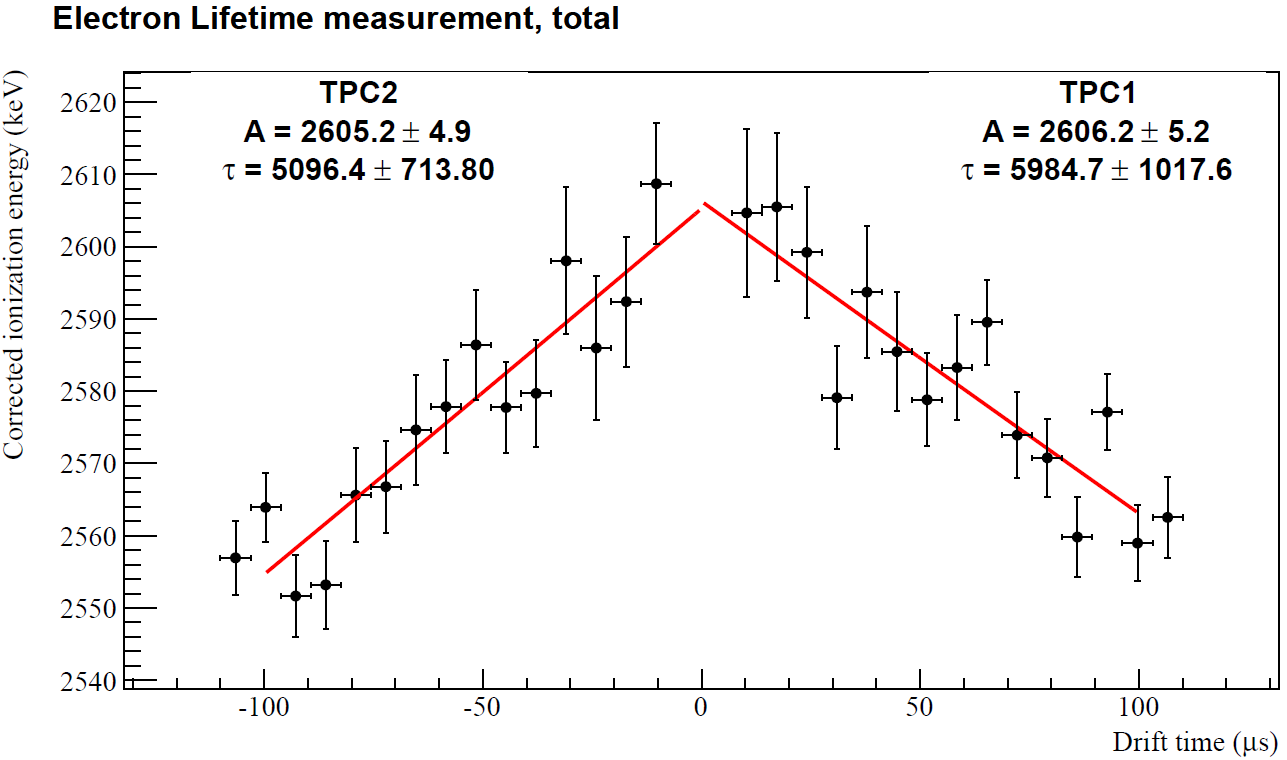
\includegraphics[keepaspectratio=true,width=\textwidth]{LongThPurityMeasurement.png}
\end{center}
\renewcommand{\baselinestretch}{1}
\small\normalsize
\begin{quote}
\caption{The purity charge correction is measured by fitting the $2615$-keV $^{208}$Tl gamma line as a function of Z-position~\cite{EnergyDocumentRun2ab}.}
\label{fig:ThPurityMeasurement}
\end{quote}
\end{figure}
\renewcommand{\baselinestretch}{2}
\small\normalsize

To extract the purity correction, the dataset is divided into time windows when the pump speed was constant and no feeds occurred; the purity is assumed to be constant during these time intervals.  It is then possible to combine all thorium source data during these time windows and fit for the $2615$-keV single-site $^{208}$Tl gamma line in Z-bins ranging from the North to the South anode.  An illustration of the ionization peak position versus Z is shown in figure~\ref{fig:ThPurityMeasurement}.  Charge attenuation is exponential with a typical $e$-fold attenuation occurring in $4-5$ ms drift time; the purity correction to charge energy is typically $2-3\%$ for charge deposits at the cathode~\cite{EnergyDocumentRun2ab}.

\begin{figure}
\begin{center}
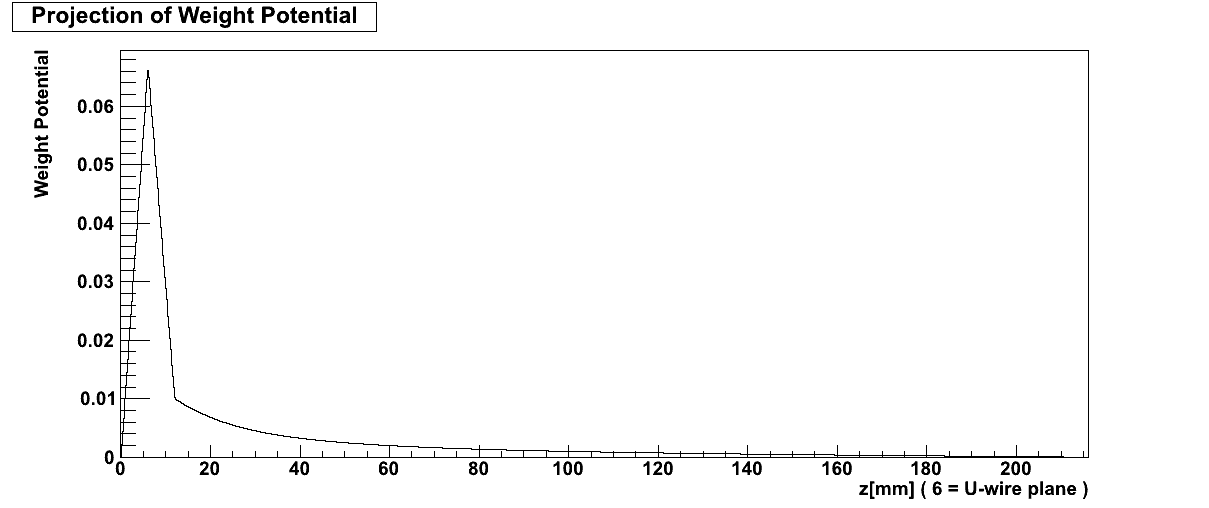
\includegraphics[keepaspectratio=true,width=\textwidth]{GridCorrectionVsZ.png}
\end{center}
\renewcommand{\baselinestretch}{1}
\small\normalsize
\begin{quote}
\caption{The expected grid correction of a u-wire as a function of $Z$-position.  In this plot, $Z = 6$ mm represents the position of the u-wire plane and $Z = 12$ mm is the position of the v-wire plane~\cite{EnergyDocumentRun2a}.}
\label{fig:GridCorrectionVsZ}
\end{quote}
\end{figure}
\renewcommand{\baselinestretch}{2}
\small\normalsize

The other Z-dependent charge correction is from the shielding grid.  Section~\ref{sec:DetectorReadout} described the process by which both electron clouds and ionized xenon will induce pulses on the wires.  The electron cloud drifts rapidly, and its pulse is observable; the ionized xenon will drift quite slowly, and will not produce an observable pulse in our electronics.  However, the ionized xenon will counteract the induced current pulse from the drifting electrons by holding some electrons on the wire; the degree to which they are able to influence the observed current pulse depends on the weight potential of the wire evaluated at the position of the xenon ions.  The simulated weight potential of a u-wire is shown as a function of Z in figure~\ref{fig:GridCorrectionVsZ}, and we can see that inside the v-wire plane this correction is expected to remain below $1\%$~\cite{EnergyDocumentRun2a}.

\begin{figure}
\begin{center}
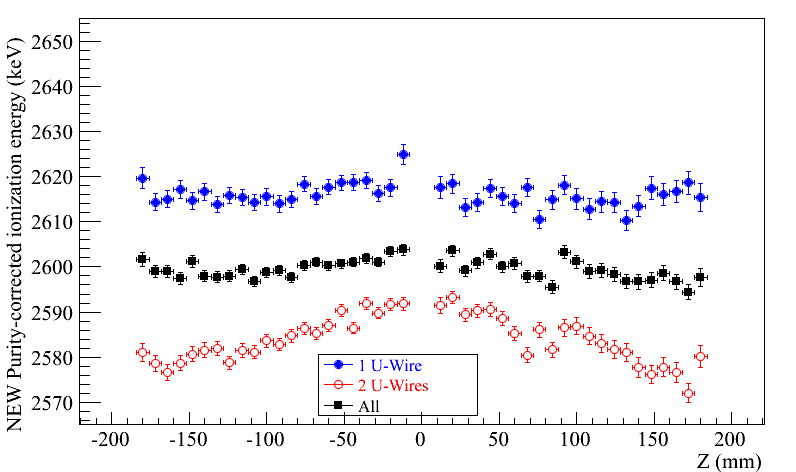
\includegraphics[keepaspectratio=true,width=\textwidth]{ResidualChargeZBias.png}
\end{center}
\renewcommand{\baselinestretch}{1}
\small\normalsize
\begin{quote}
\caption{After applying all charge corrections, we find that the $2615$-keV $^{208}$Tl ionization peak is observed at the expected location for single-wire events; however, for two-wire events a residual bias is observed which also exhibits Z-dependence~\cite{EnergyDocumentRun2ab}.}
\label{fig:ResidualChargeZBias}
\end{quote}
\end{figure}
\renewcommand{\baselinestretch}{2}
\small\normalsize

These are all of the known corrections to the charge energy.  However, we find that after applying them, there remains a residual z-dependence in the charge calibration.  Figure~\ref{fig:ResidualChargeZBias} shows that although the $2615$-keV $^{208}$Tl ionization peak has been properly corrected for clusters which deposit on only one u-wire, for clusters which are split between two u-wires there is a residual offset in peak position of roughly $1\%$ and an additional z-dependent effect of up to roughly $0.3\%$.  These effects are not presently understood; however, they are believed to induce a Z-dependent bias effect in the lightmap which is used for scintillation denoising, which in turn is believed to cause the scintillation z-bias described in section~\ref{sec:ResultEnergyLight}~\cite{EnergyDocumentRun2ab}.  Active work is underway to understand this z-bias in charge and develop an appropriate correction.

\subsection{Light Corrections}\label{sec:ResultEnergyLight}

Although scintillation measurements are made from fitting the magnitudes of the scintillation pulses found on the summed North and South APD planes in reconstruction, as described in section~\ref{sec:ReconPulseFitting}, these scintillation measurements are superseded by the denoised scintillation energies estimated using the denoising method of chapter~\ref{ch:DenoisingTheory}.  This subsection will describe evaluations of the success of that denoising effort and subsequent corrections made to the denoised scintillation energy.

\begin{figure}
\begin{center}
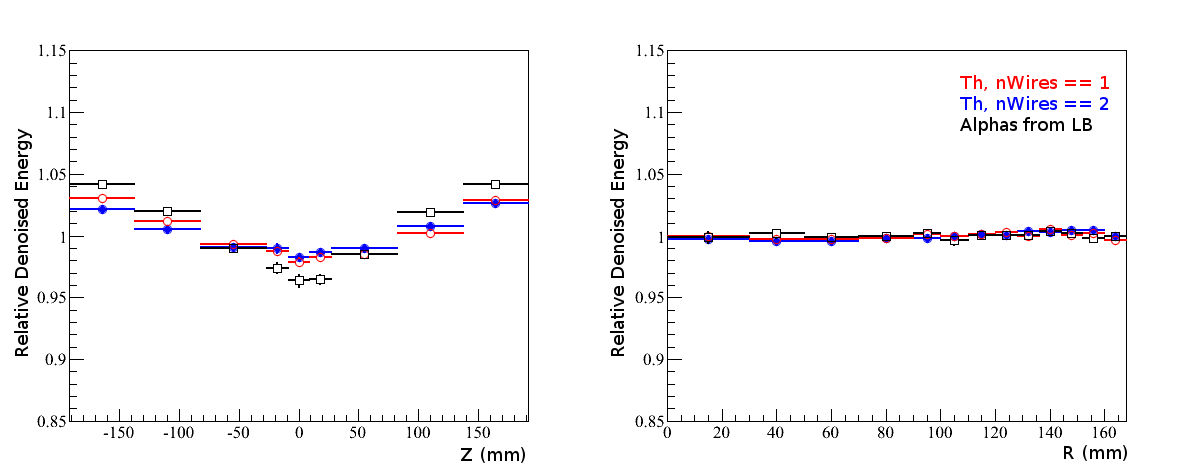
\includegraphics[keepaspectratio=true,width=\textwidth,clip=true,trim=0mm 0mm 20mm 0mm]{DenoisedScintillatonRelativeRZBias.png}
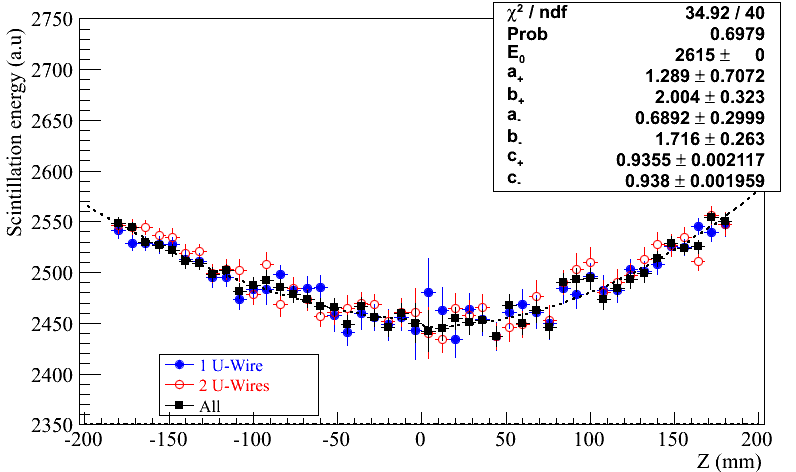
\includegraphics[keepaspectratio=true,width=\textwidth]{DenoisedScintillatonZBias.png}
\end{center}
\renewcommand{\baselinestretch}{1}
\small\normalsize
\begin{quote}
\caption{A residual calibration offset and Z-dependent behavior is observed in the denoised scintillation measurements.  The top plots show the relative peak position of the scintillation-only $2615$-keV $^{208}$Tl peak (one-wire and two-wire) and average alpha energy from $^{222}$Rn versus Z (top left) and R (top right).  The bottom plot shows the absolute denoised scintillation energy from the $2615$-keV $^{208}$Tl peak for one and two wires, with the measured correction function overlaid~\cite{EnergyDocumentRun2ab}.}
\label{fig:ResidualLightZBias}
\end{quote}
\end{figure}
\renewcommand{\baselinestretch}{2}
\small\normalsize

When the denoising algorithm operates properly, it should be constrained to produce scintillation energy measurements calibrated in keV.  This calibration is accomplished by the lightmap, which retains information about the magnitude of pulses produced by $2615$-keV energy deposits.  However, in practice it is seen that the denoised scintillation measurements are not properly calibrated; this can be seen in figure~\ref{fig:ResidualLightZBias}, where it is clear that events of all types (alpha decays in low-background data and both one-wire and two-wire single-site gamma decays from an external source) measure a scintillation energy which is systematically too low and displays significant Z-dependence.  The thorium data, which provides more the best measurement statistics, shows a mis-calibration which ranges from $2.5\%$ near the anodes to $6.5\%$ at the cathode~\cite{EnergyDocumentRun2ab}.

The cause for the discrepancy in scintillation energy measurements is not currently known.  One hypothesis is that the discrepancy in two-wire charge cluster measurements described in section~\ref{sec:ResultEnergyCharge} may lead to inaccurate event selection in the generation of the lightmap described in section~\ref{sec:LightmapEventSelection}; poor event selection would lead to a systematic error in the lightmap which could depend on Z, and would be capable of creating the observed bias.  Attempts to address this Z-bias within the generation of the lightmap or investigate alternative explanations for its origin have so far been unsuccessful, but these investigations continue, and it is hoped that this issue can be fixed for the next analysis.

For the present analysis an empirical correction of the discrepancy is applied.  The scintillation correction function takes the form:
\begin{equation}
E_{corr} = E_{meas}\cdot \begin{cases}
\left[ (c_{-}) + (a_{-})\cdot |Z|^{b_{-}} \right]^{-1} & \text{if } Z < 0\\
\left[ (c_{+}) + (a_{+})\cdot |Z|^{b_{+}} \right]^{-1} & \text{if } Z > 0,
\end{cases}\end{equation}
where we measure from data $c_{-} = 0.9380$, $c_{+} = 0.9355$, $b_{-} = 1.71$, $b_{+} = 2.00$, $a_{-} = 0.69$, $a_{+} = 1.3$, and $Z$ is in units of meters.  The bottom plot of figure~\ref{fig:ResidualLightZBias} shows this empirical correction overlaid on one-wire and two-wire thorium source data, demonstrating that the function agrees well with the observed Z-dependent offset~\cite{EnergyDocumentRun2ab}.

\subsection{Rotated Energy Calibration}\label{sec:RotatedEnergyCalibration}

From the corrected scintillation and charge energy measurements, it is necessary to form a calibrated rotated energy measurement which combines them.  This combination takes advantage of anticorrelation between charge and light to achieve an optimal energy resolution.  To accomplish these measurements, it is necessary to use multiple calibration points; we use the $2615$-keV gamma line from regularly-taken thorium source runs to measure time-dependent calibration parameters and the 662-keV cesium and $1173$-keV and $1332$-keV cobalt gamma lines from source runs to characterize the energy dependence of calibrations.  The linear combination of scintillation and charge is selected to optimize the energy resolution of the thorium line; the precise measurement of energy resolution is described in section~\ref{sec:RotatedEnergyResMeasurement}, but for this purpose we simply seek to make energy peaks as narrow as possible.

The calibrated rotated energy $E$ is computed by a calibration function of the form:
\begin{subequations}\label{eqn:EnergyCalibrationParametrization}\begin{align}
E_{rot} &= E_S \cdot sin(\theta(t)) + E_C \cdot cos(\theta(t))\\
E_{ratio} &= \frac{E_{rot}}{E^{th}_{rot}(t)}\\
E &= \left( E_{thorium} - E_{bias} \right) \cdot \left( p_0 + p_1 E_{ratio} + p_2 E_{ratio}^2\right),
\end{align}\end{subequations}
where $E_C$ and $E_S$ are the measured charge and scintillation energies (with corrections applied as described in sections~\ref{sec:ResultEnergyCharge} and \ref{sec:ResultEnergyLight}), $\theta(t)$ is a time-dependent rotation angle measured to optimize the fractional energy resolution of the thorium gamma line, $E^{th}_{rot}(t)$ is the time-dependent location of the thorium peak in the spectrum of $E_{rot}$, $E_{thorium}$ is the true thorium peak position equal to $2615$ keV, and $E_{bias}$, $p_0$, $p_1$, and $p_2$ are time-independent calibration parameters.  Entirely separate calibration parameters are obtained for single-site and multi-site events.

\begin{figure}
\begin{center}
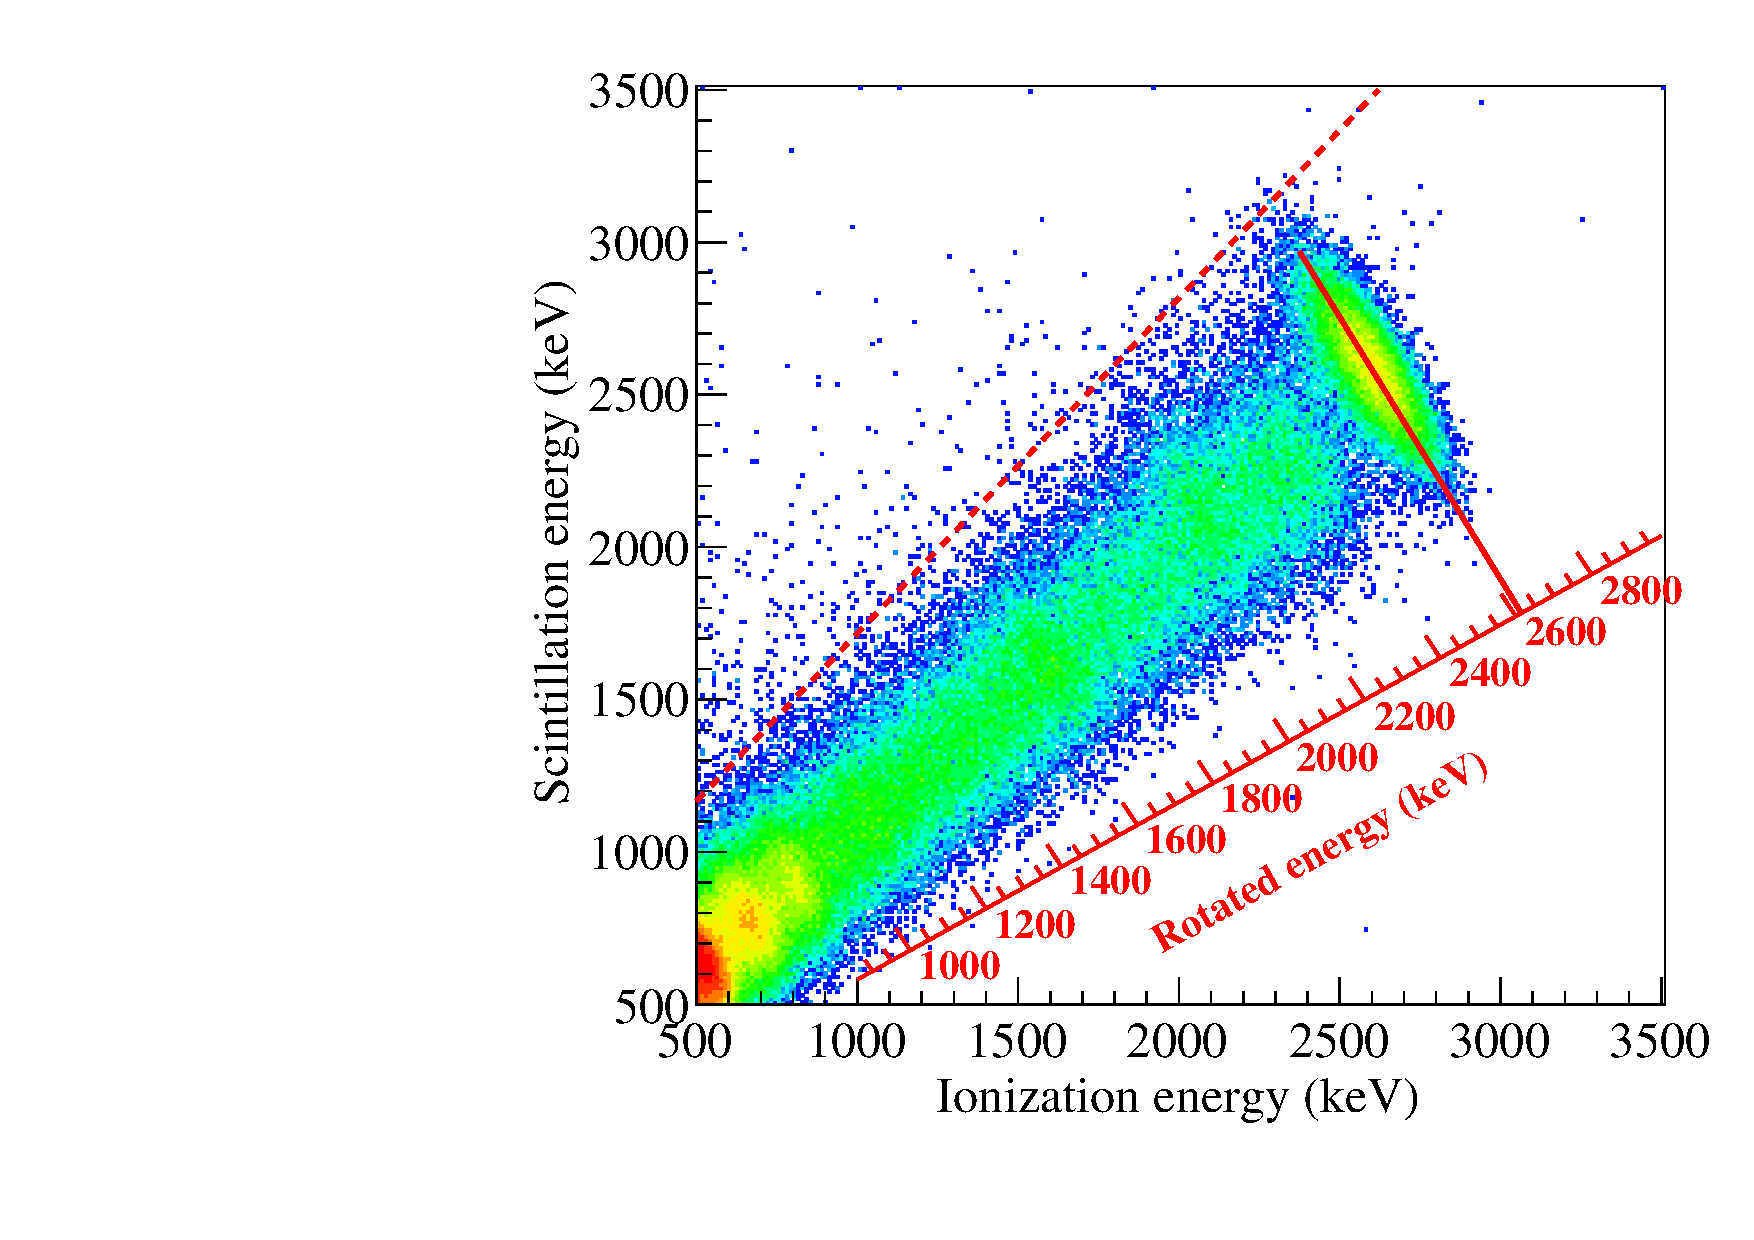
\includegraphics[keepaspectratio=true,width=\textwidth]{RotationTh2D_withCalibration.pdf}
\end{center}
\renewcommand{\baselinestretch}{1}
\small\normalsize
\begin{quote}
\caption{Corrected scintillation versus charge energy are shown for a thorium run.  The projection angle for the rotated energy measurement is illustrated at the $2615$-keV peak; the projection onto a calibrated axis is shown.  The dotted red line indicates the diagonal cut described in section~\ref{sec:ResultFitting}.  Figure provided by Liangjian Wen.}
\label{fig:LiangjianAnticorrelatedEnergy}
\end{quote}
\end{figure}
\renewcommand{\baselinestretch}{2}
\small\normalsize

\begin{figure}
\begin{center}
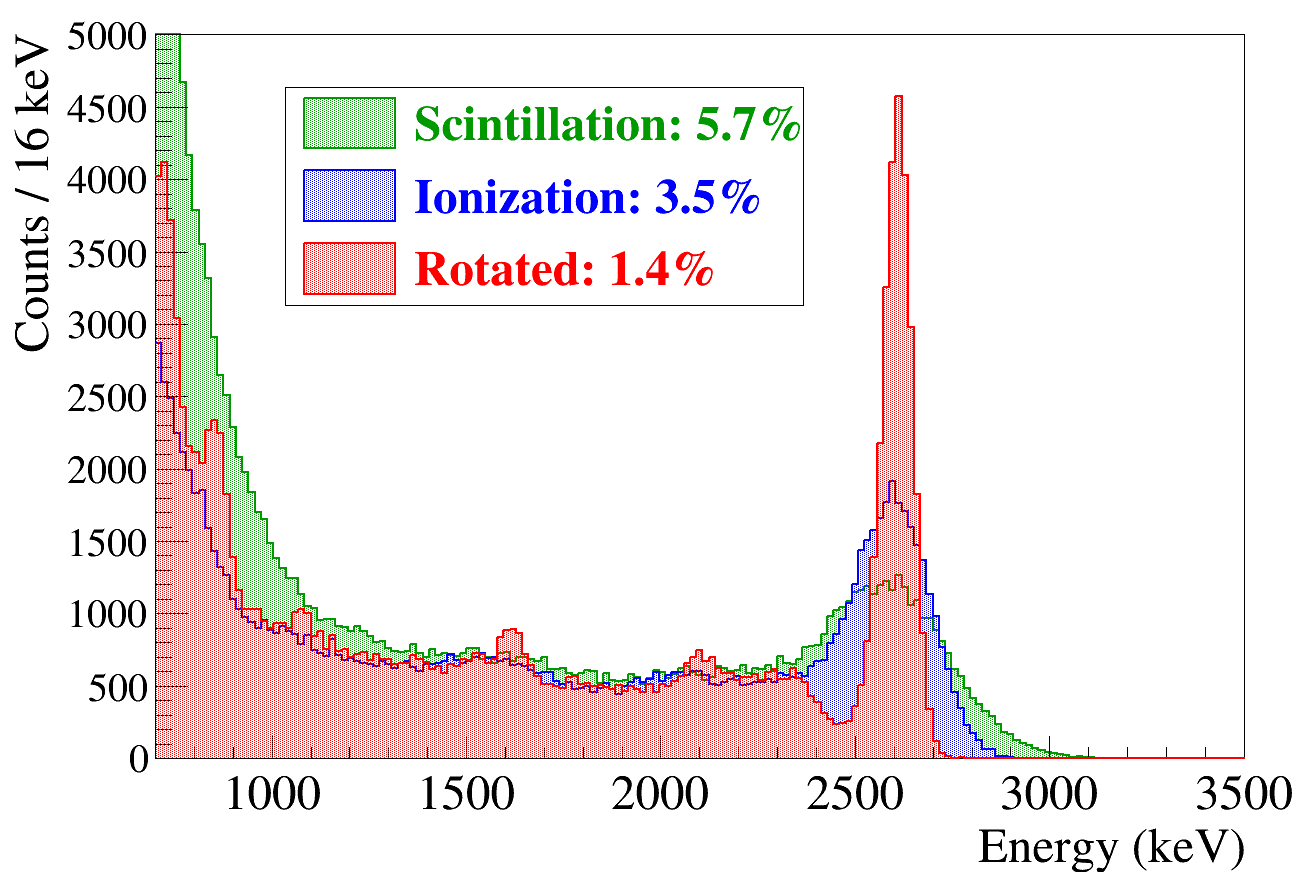
\includegraphics[keepaspectratio=true,width=\textwidth]{RotationTh2D_ImprovementInResolution.png}
\end{center}
\renewcommand{\baselinestretch}{1}
\small\normalsize
\begin{quote}
\caption{Charge-only, scintillation-only, and rotated energy spectra are shown from a thorium source run; the significant improvement in energy resolution with the rotated energy measurement is apparent, as are low-energy features which are washed out in the lower-resolution spectra.  Figure provided by Liangjian Wen.}
\label{fig:LiangjianRotatedSpectrumImprovement}
\end{quote}
\end{figure}
\renewcommand{\baselinestretch}{2}
\small\normalsize

The result of this calibration is shown in figure~\ref{fig:LiangjianAnticorrelatedEnergy}.  We can see here that a projection is performed from the two-dimensional charge-light spectrum along an axis that minimizes the width of the thorium gamma line.  Figure~\ref{fig:LiangjianRotatedSpectrumImprovement} demonstrates the spectra we obtain from projections only in scintillation, only in ionization, and using the optimal linear combination we have described; the improvement in resolution from using an appropriate linear combination of scintillation and ionization is apparent, as the peak at $2615$ keV becomes sharper and additional low-energy features of the spectrum become apparent which were washed out with worse resolution.  The next section will describe the process of measuring the energy resolution.

\subsection{Measurement of Rotated Energy Resolution}\label{sec:RotatedEnergyResMeasurement}

The previous section has described the calibration of the rotated energy spectrum.  In this section, we describe the measurement of energy resolution with this rotated energy measurement.

The resolution is assumed to be energy-dependent; if a monoenergetic deposit is made in the liquid xenon, we hypothesize that the observed spectrum should be Gaussian and define the energy resolution at that energy to be the value of $\sigma$.  We can parametrize the dependence of $\sigma$ on energy as:
\begin{equation}\label{eqn:ResolutionAbsoluteFunctionForm}
\sigma(E) = \sqrt{p_0^2 E + p_1^2 + p_2^2 E^2},
\end{equation}
where typically we interpret the parameters $p_1$ to come from electronic noise (which contributes a smearing independent of energy), $p_0$ to come from statistical fluctuations in the number of photons or electrons observed (which follows a Poisson distribution in the number of photons), and $p_2$ to come from mis-calibration of components of the detector (whose effect increases linearly with the size of the pulse)~\cite{knoll2000radiation}.  We also often find it useful to refer to the relative or fractional energy resolution, defined as:
\begin{equation}
\sigma(E)/E = \sqrt{p_0^2/E + p_1^2/E^2 + p_2^2}.
\end{equation}
The resolutions of single-site and multi-site events differ, so there are separate resolution functions measured for both classes of events.

\begin{table}
\begin{center}
\begin{tabular}{|c|c|c|}
\hline Parameter & SS & MS \\
\hline $p_0$ & 0.628 & 0.602 \\
\hline $p_1$ & 20.8 & 25.8 \\
\hline $p_2$ & 0.0011 & 0.0040 \\ \hline
\end{tabular}
\end{center}
\caption{Time-averaged resolution parameters for the single-site and multi-site denoised dataset~\cite{AverageEnergyResolutionDocument}.}
\label{tab:ResolutionFunctions_DenoisedOnly}
\end{table}

\begin{figure}
\begin{center}
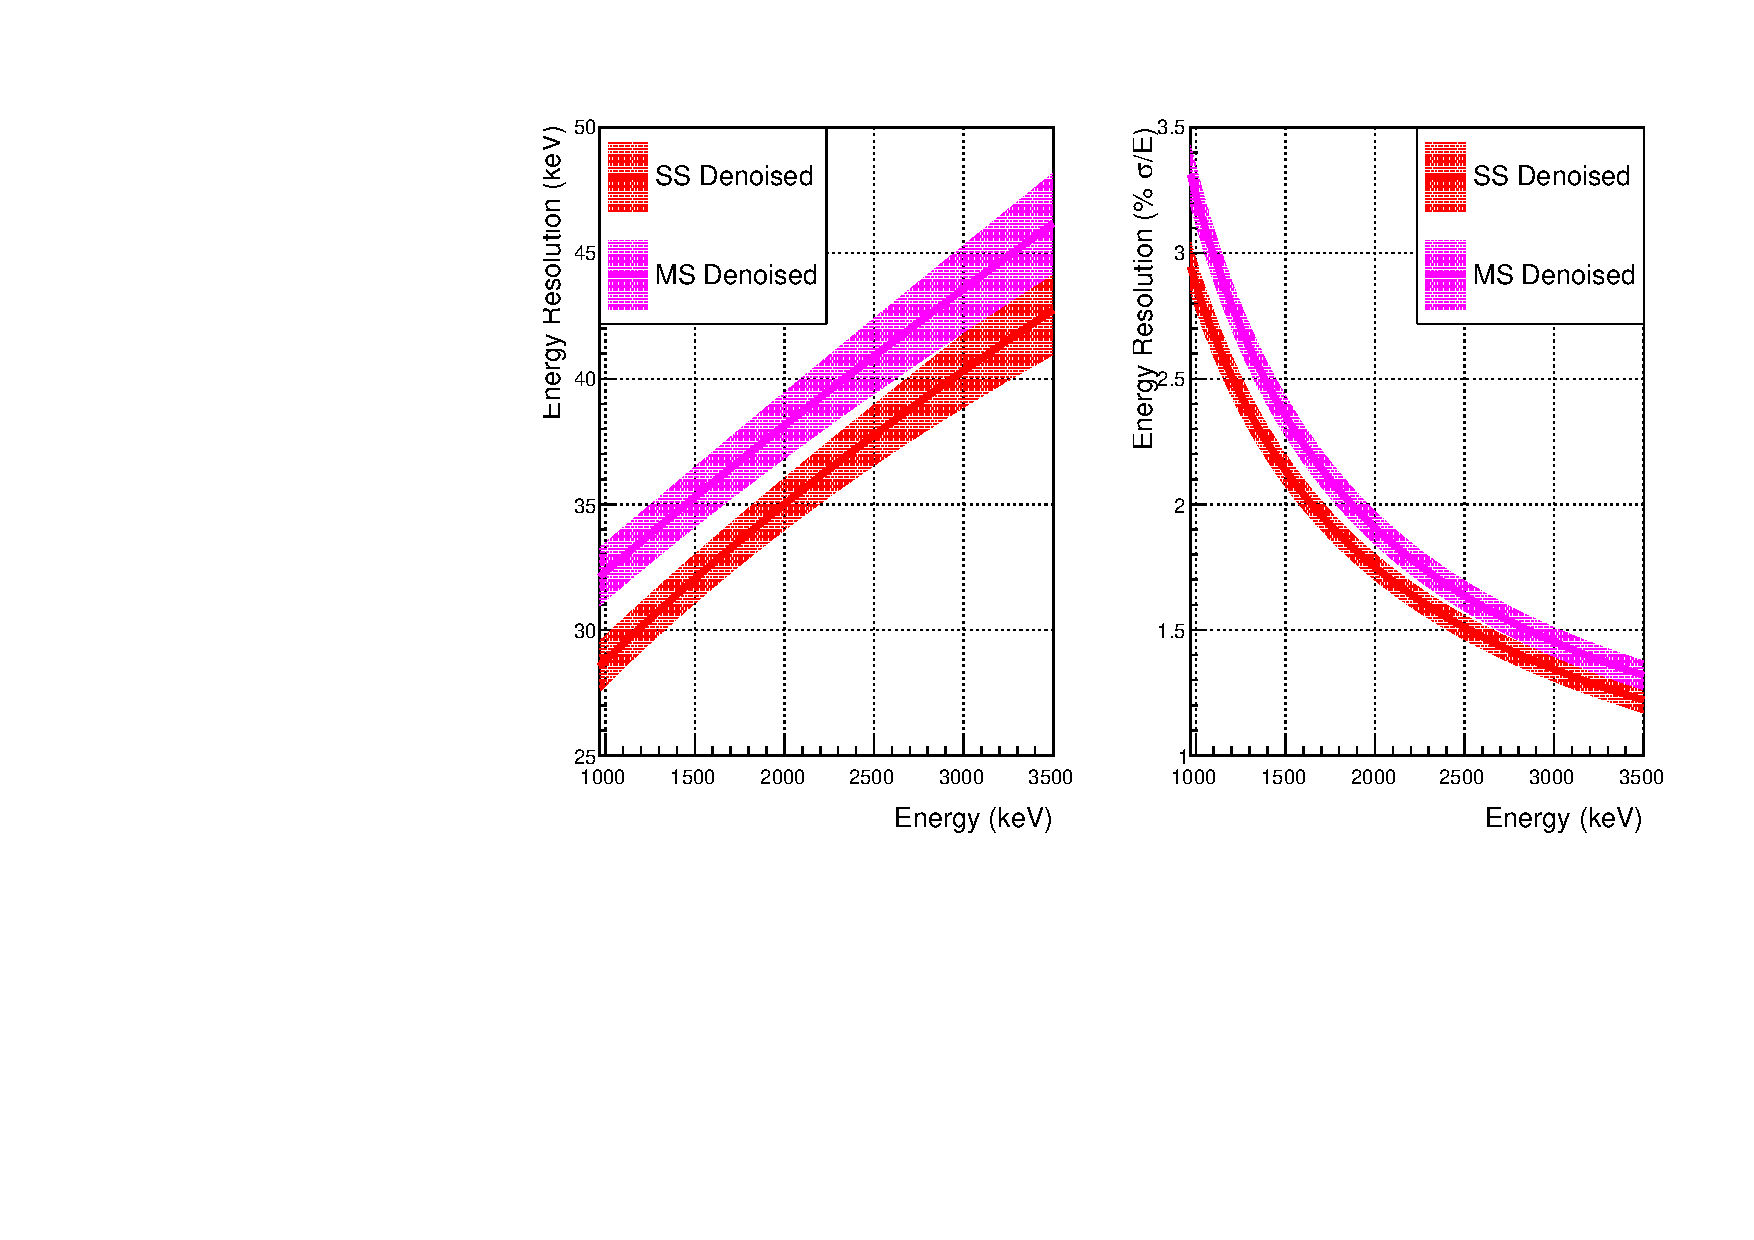
\includegraphics[keepaspectratio=true,width=\textwidth]{ResolutionDenoisedOnly.pdf}
\end{center}
\renewcommand{\baselinestretch}{1}
\small\normalsize
\begin{quote}
\caption{The time-averaged resolution functions (left) and relative resolution functions (right) for single-site (red) and multi-site (purple) denoised data.  Shaded bands indicate uncertainties.  Data provided by Caio Licciardi.}
\label{fig:ResolutionFunctionComparison_DenoisedOnly}
\end{quote}
\end{figure}
\renewcommand{\baselinestretch}{2}
\small\normalsize

The resolution functions are measured using only the cobalt and thorium calibration gamma lines (at $1173$, $1332$, and $2615$ keV).  The resolution parameters are time-dependent; average resolution parameters are computed by weighting the resolutions observed in different time windows by the fraction of EXO-200 low-background data taken within that window.  The resulting resolution parameters are listed in table~\ref{tab:ResolutionFunctions_DenoisedOnly}.  Figure~\ref{fig:ResolutionFunctionComparison_DenoisedOnly} shows the resulting resolution functions.  We can see that at our typical energies of $\approx 2500$ keV the $p_0$ and $p_1$ terms dominate the resolution function of equation~\ref{eqn:ResolutionAbsoluteFunctionForm}, and this manifests itself as a concave-downward shape in the absolute resolution function.  The shape of these resolution curves can be interpreted as meaning that the electronic noise and Poisson fluctuations dominate our resolution; this may not be surprising, since we recall from section~\ref{sec:DenoisingInPractice} that Poisson fluctuations were underweighted in the version of denoising implemented for this analysis.  Our interpretation is only suggestive because the curvature is slight and the energy-dependent calibration effects cannot be ruled out, but it will be interesting to see how these terms change when future work addresses the underweighting of Poisson fluctuations.

\begin{figure}
\begin{center}
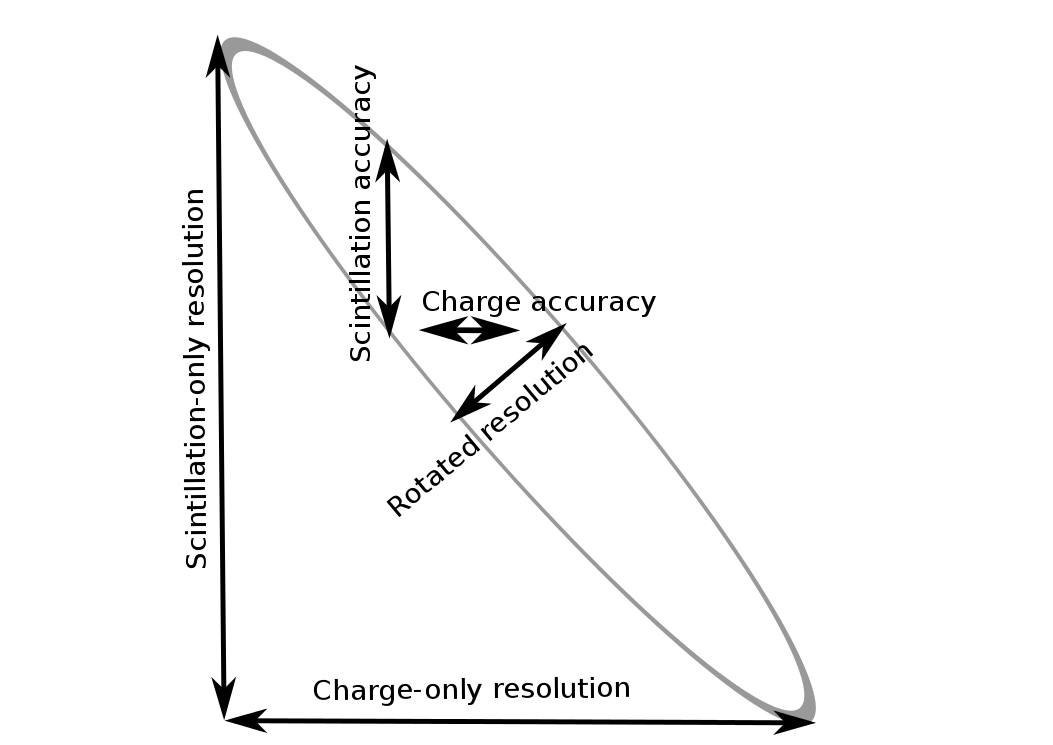
\includegraphics[keepaspectratio=true,width=.7\textwidth]{RotatedIsland.png}
\end{center}
\renewcommand{\baselinestretch}{1}
\small\normalsize
\begin{quote}
\caption{A typical monoenergetic gamma line, where the horizontal axis indicates ionization energy and the vertical axis indicates scintillation energy.  We note that the ionization-only and scintillation-only resolutions are dominated by the length and angle of the island, which are dominated by xenon physics and the choice of electric field rather than the accuracy of the readouts in those channels.}
\label{fig:RotatedIslandSchematic}
\end{quote}
\end{figure}
\renewcommand{\baselinestretch}{2}
\small\normalsize

\begin{figure}
\begin{center}
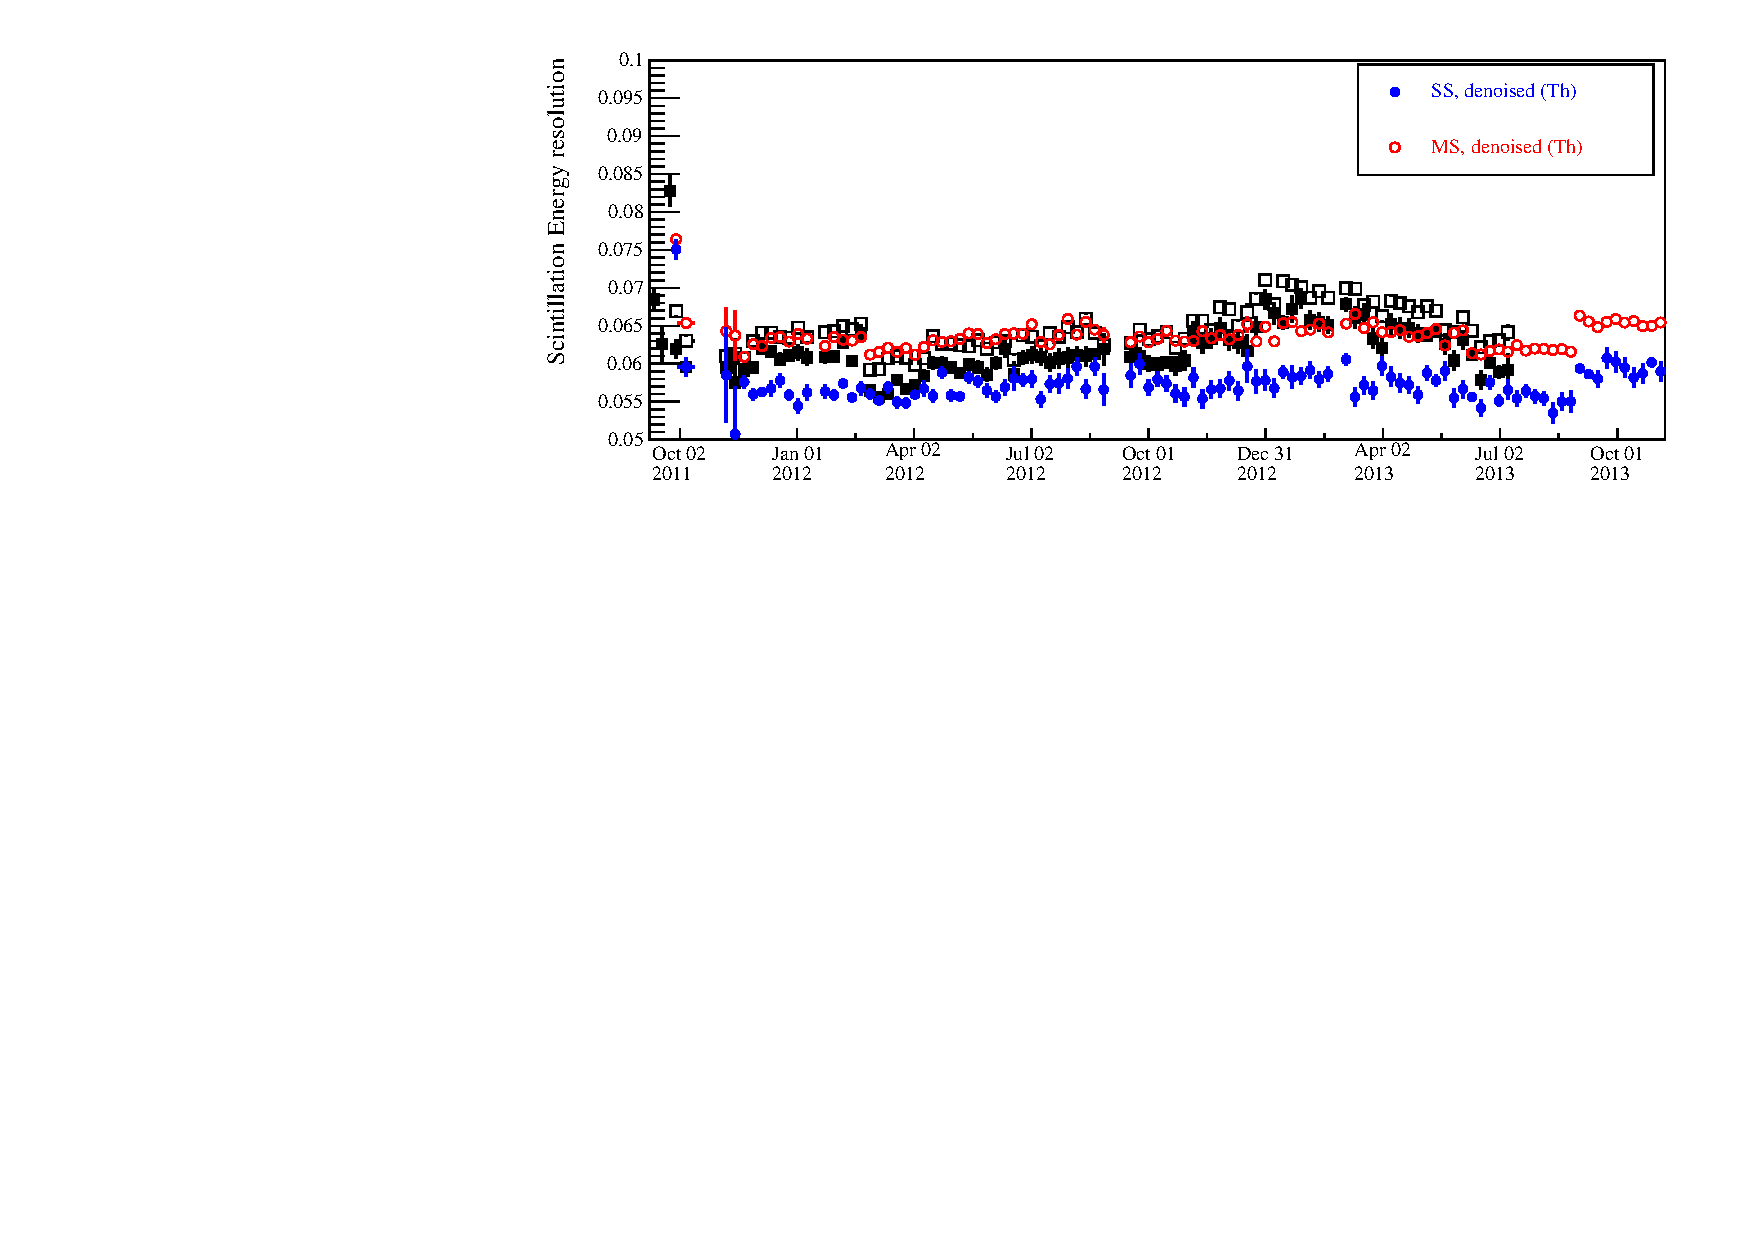
\includegraphics[keepaspectratio=true,width=\textwidth]{scint_resolutions_denoised.pdf}
\end{center}
\renewcommand{\baselinestretch}{1}
\small\normalsize
\begin{quote}
\caption{Scintillation-only resolution over time, including: single-site denoised (blue), multi-site denoised (red), single-site undenoised (black solid), multi-site undenoised (hollow square).  Although denoising does show some improvement in the scintillation-only resolution, it is quite modest; this is because the scintillation-only resolution is dominated by fluctuations in light yield.~\cite{EnergyDocumentRun2ab}.}
\label{fig:ScintillationOnlyResolutionTrend}
\end{quote}
\end{figure}
\renewcommand{\baselinestretch}{2}
\small\normalsize

It may be tempting, given that the topic of this work is a system for denoising scintillation waveforms, to prefer to focus on the scintillation-only resolution.  However, the scintillation-only resolution is in fact dominated not by the accuracy of the readout system but by fluctuations in the fraction of deposited energy which is released in the scintillation channel.  Figure~\ref{fig:RotatedIslandSchematic} shows a schematic of a typical monoenergetic gamma line; the length and angle of the island represents the anticorrelation between light and charge.  We can see that although the charge and light yield are highly correlated, individually they are also subject to significant fluctuations.  A scintillation-only energy measurement is fundamentally limited by these fluctuations in light yield, and only to second order is it affected by the accuracy of our event-by-event measurements of light yield.  A comparison between the denoised and undenoised scintillation-only resolution can be seen in figure~\ref{fig:ScintillationOnlyResolutionTrend}, and as expected the improvement from denoising is quite modest.  Considering that the scintillation-only energy measurement is not used in the final analysis and does not provide a window onto the performance of denoising, we will not consider it further in this work.

\subsection{Cross-Checks on the Energy Calibration}

The energy calibration is extracted from source data; the large quantity of source data leads to small statistical errors on the calibration constants.  However, the calibration constants are time-dependent and it is valuable to have cross-checks verifying that the time-dependent nature of the calibration is accounted for properly.

To cross-check the time-dependence of the calibrations derived from sources, we use gamma lines in the low-background data.  These can verify that gamma lines from a wide range of times are combined to produce coherent peaks in our cumulative energy spectrum; they can also verify that the time-averaged resolutions extracted from source data are accurate because the resolution extracted from low-background peaks is inherently averaged over the duration of the data run.  Two energy lines from the low-background spectrum have been identified as particularly useful.

\begin{figure}
\begin{center}
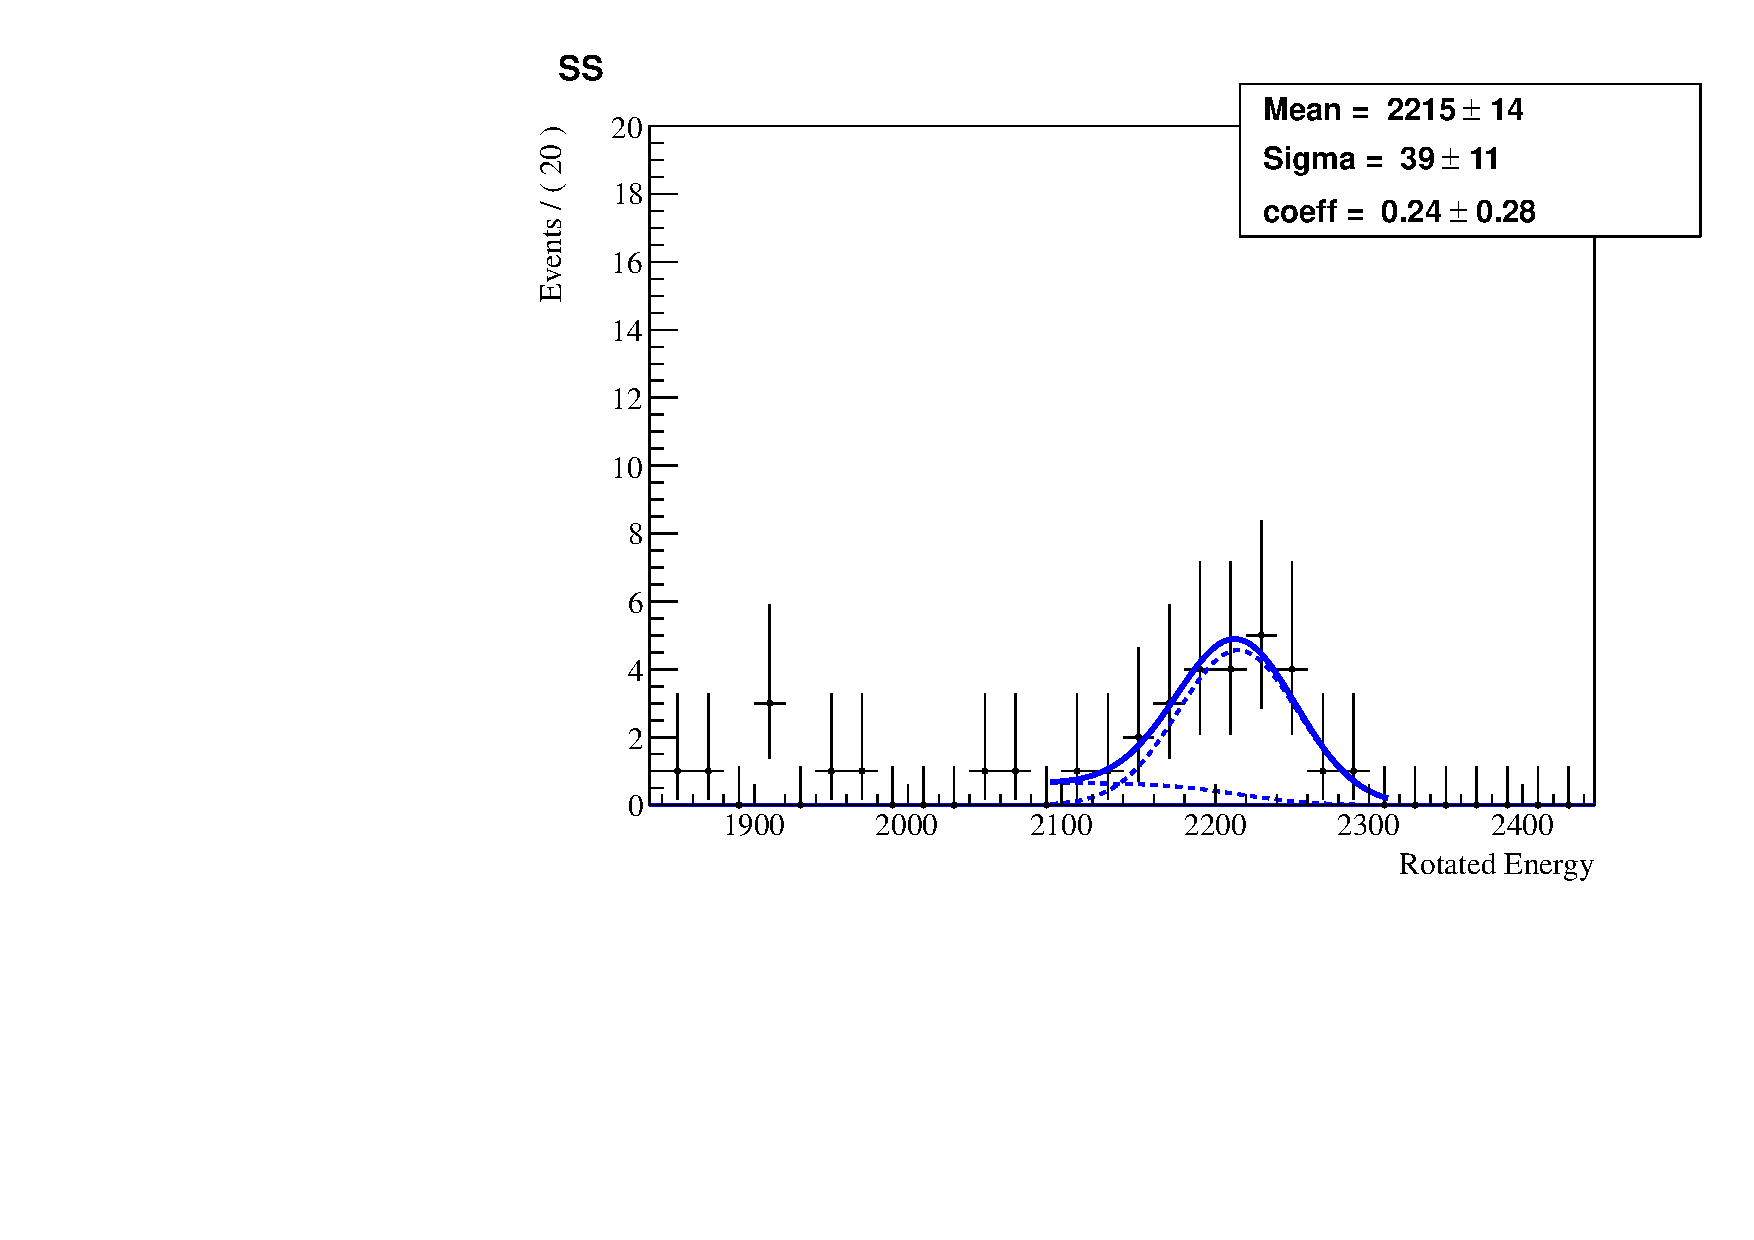
\includegraphics[keepaspectratio=true,width=.49\textwidth]{neutronHydrogen_ss_denoised.pdf}
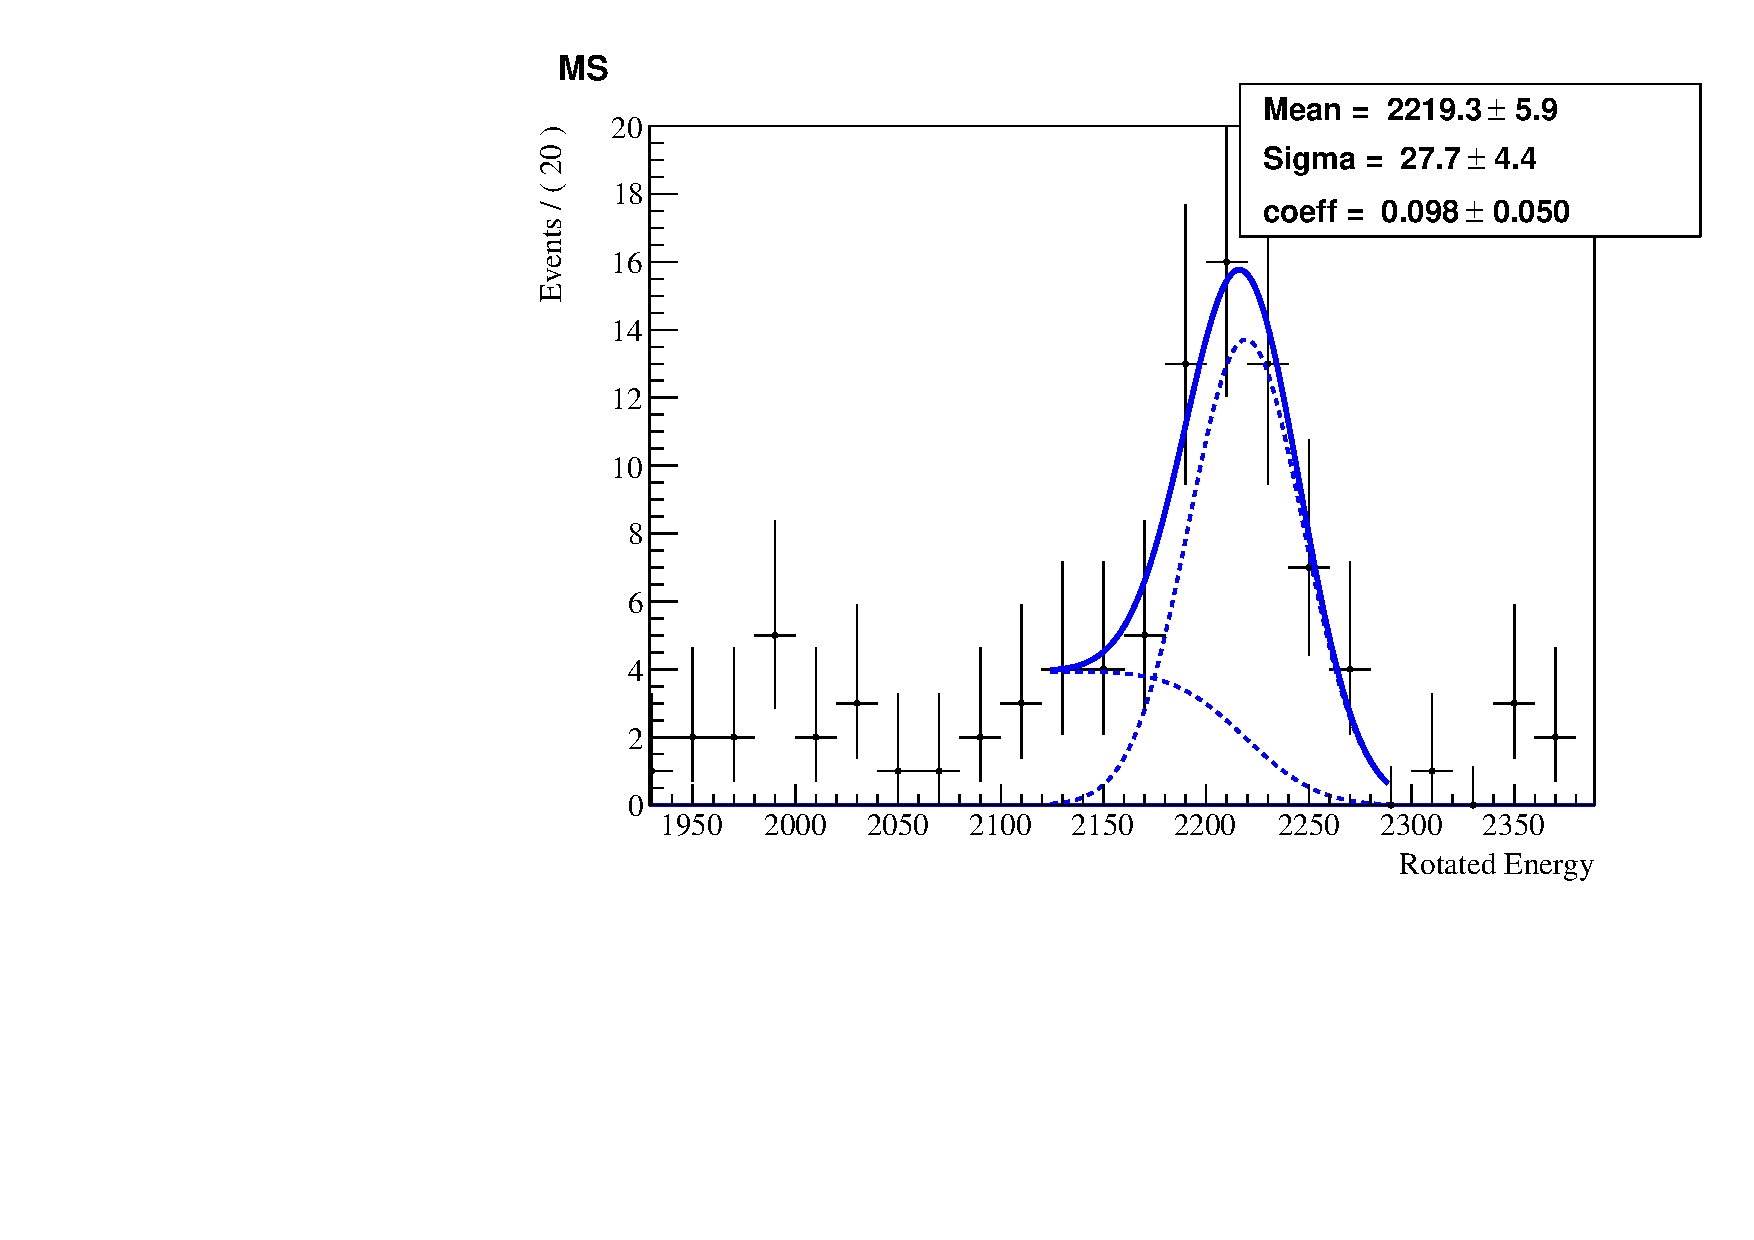
\includegraphics[keepaspectratio=true,width=.49\textwidth]{neutronHydrogen_ms_denoised.pdf}
\end{center}
\renewcommand{\baselinestretch}{1}
\small\normalsize
\begin{quote}
\caption{The single-site (left) and multi-site (right) gamma line at $2.2$ MeV from neutron capture on hydrogen can be used as a low-background cross-check on the resolution calibration.  Here, data which is coincident with a muon veto is shown to include the expected neutron capture peak~\cite{EnergyDocumentRun2ab}.}
\label{fig:neutronHydrogenCheck}
\end{quote}
\end{figure}
\renewcommand{\baselinestretch}{2}
\small\normalsize

One gamma line in the low-background data comes from neutron capture on hydrogen in the HFE-7000 refrigerant.  Such events are generally vetoed by the coincidence cuts, primarily the veto panels, so their impact on the low-background data is suppressed; conversely, it is possible to study only events which occur in coincidence with muon detection by the veto panels, thereby enriching our dataset in neutron capture spectra.  Neutron capture on hydrogen emits a $2.2$ MeV gamma; figure~\ref{fig:neutronHydrogenCheck} shows the data which is produced by this source with a fit to a Gaussian function and simple background model.~\cite{NeutronCaptureGammas,EnergyDocumentRun2ab}.

\begin{figure}
\begin{center}
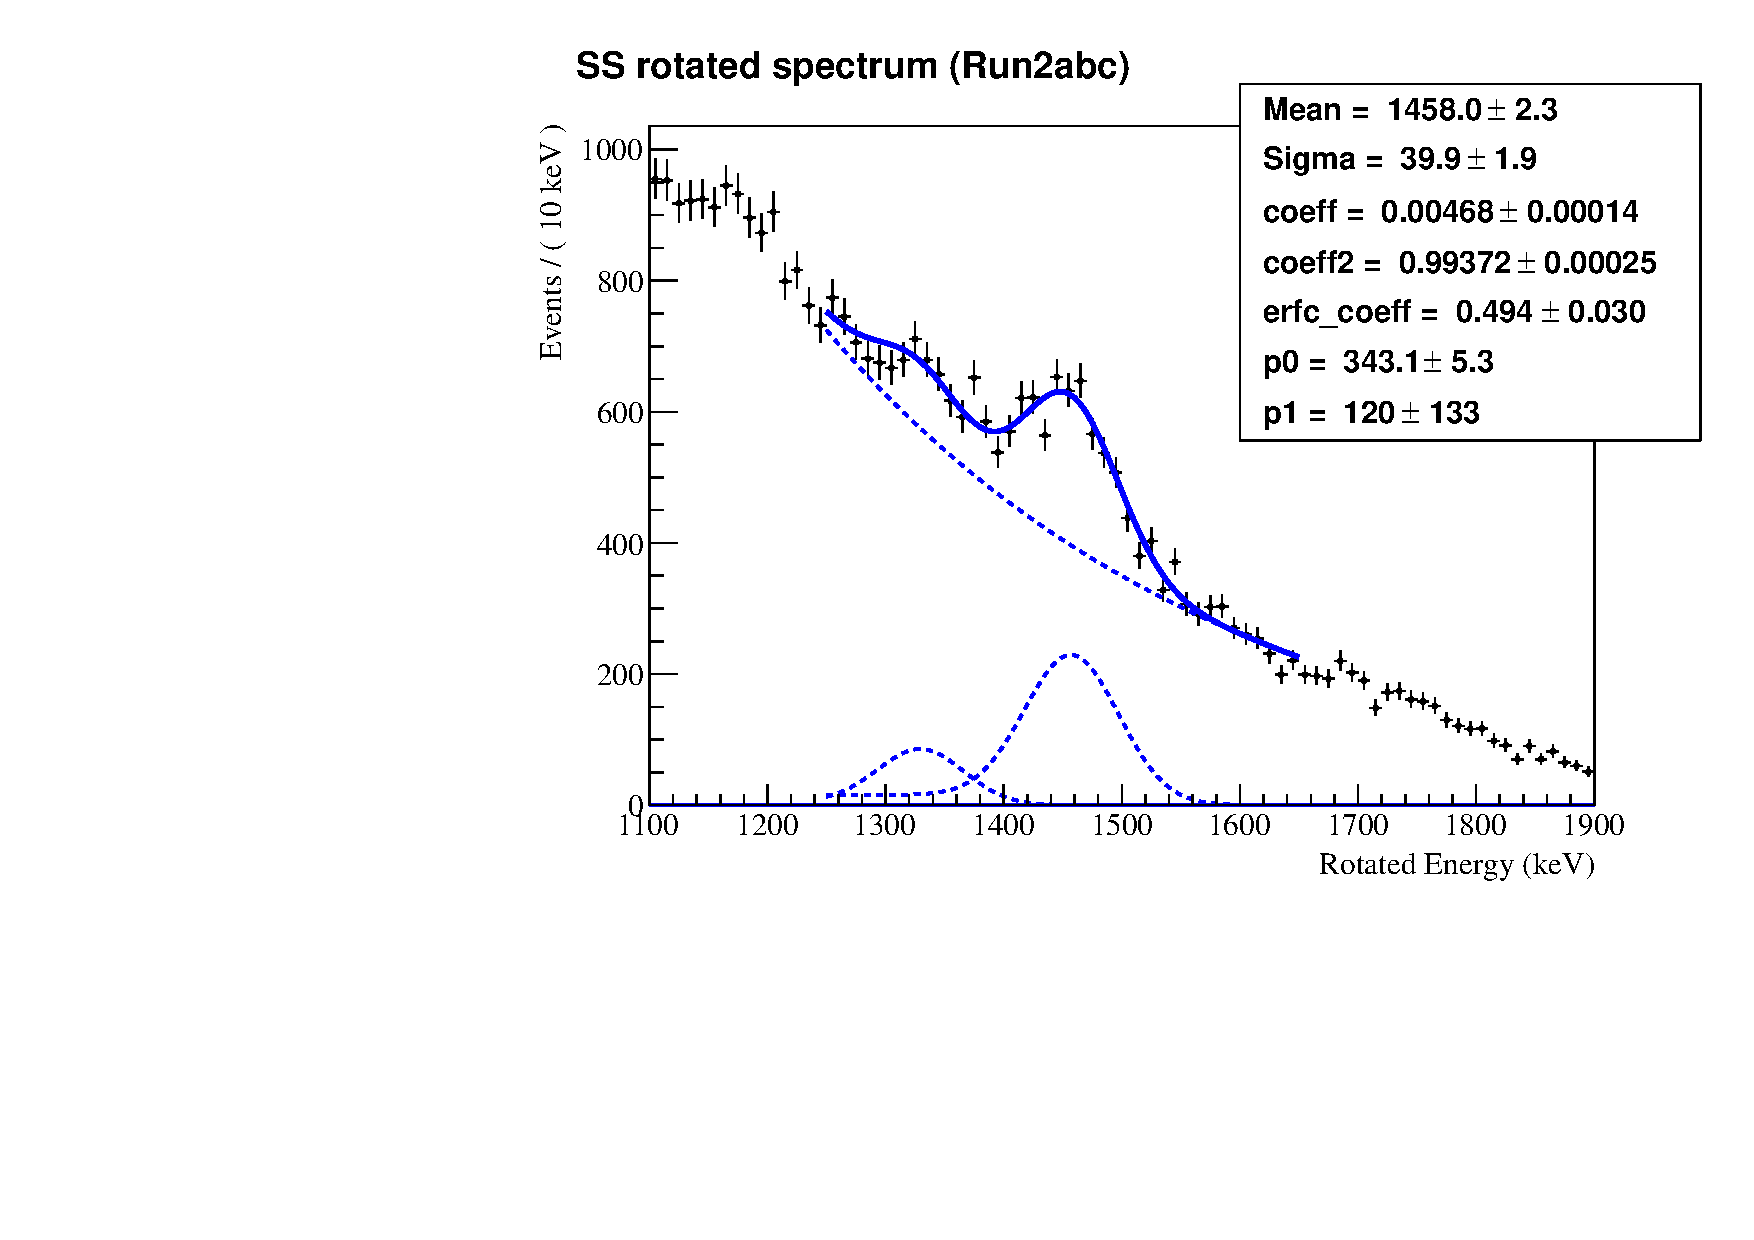
\includegraphics[keepaspectratio=true,width=.49\textwidth]{EXO_Workspace_Run2abc_K40_ss_1250keVto1650keV.pdf}
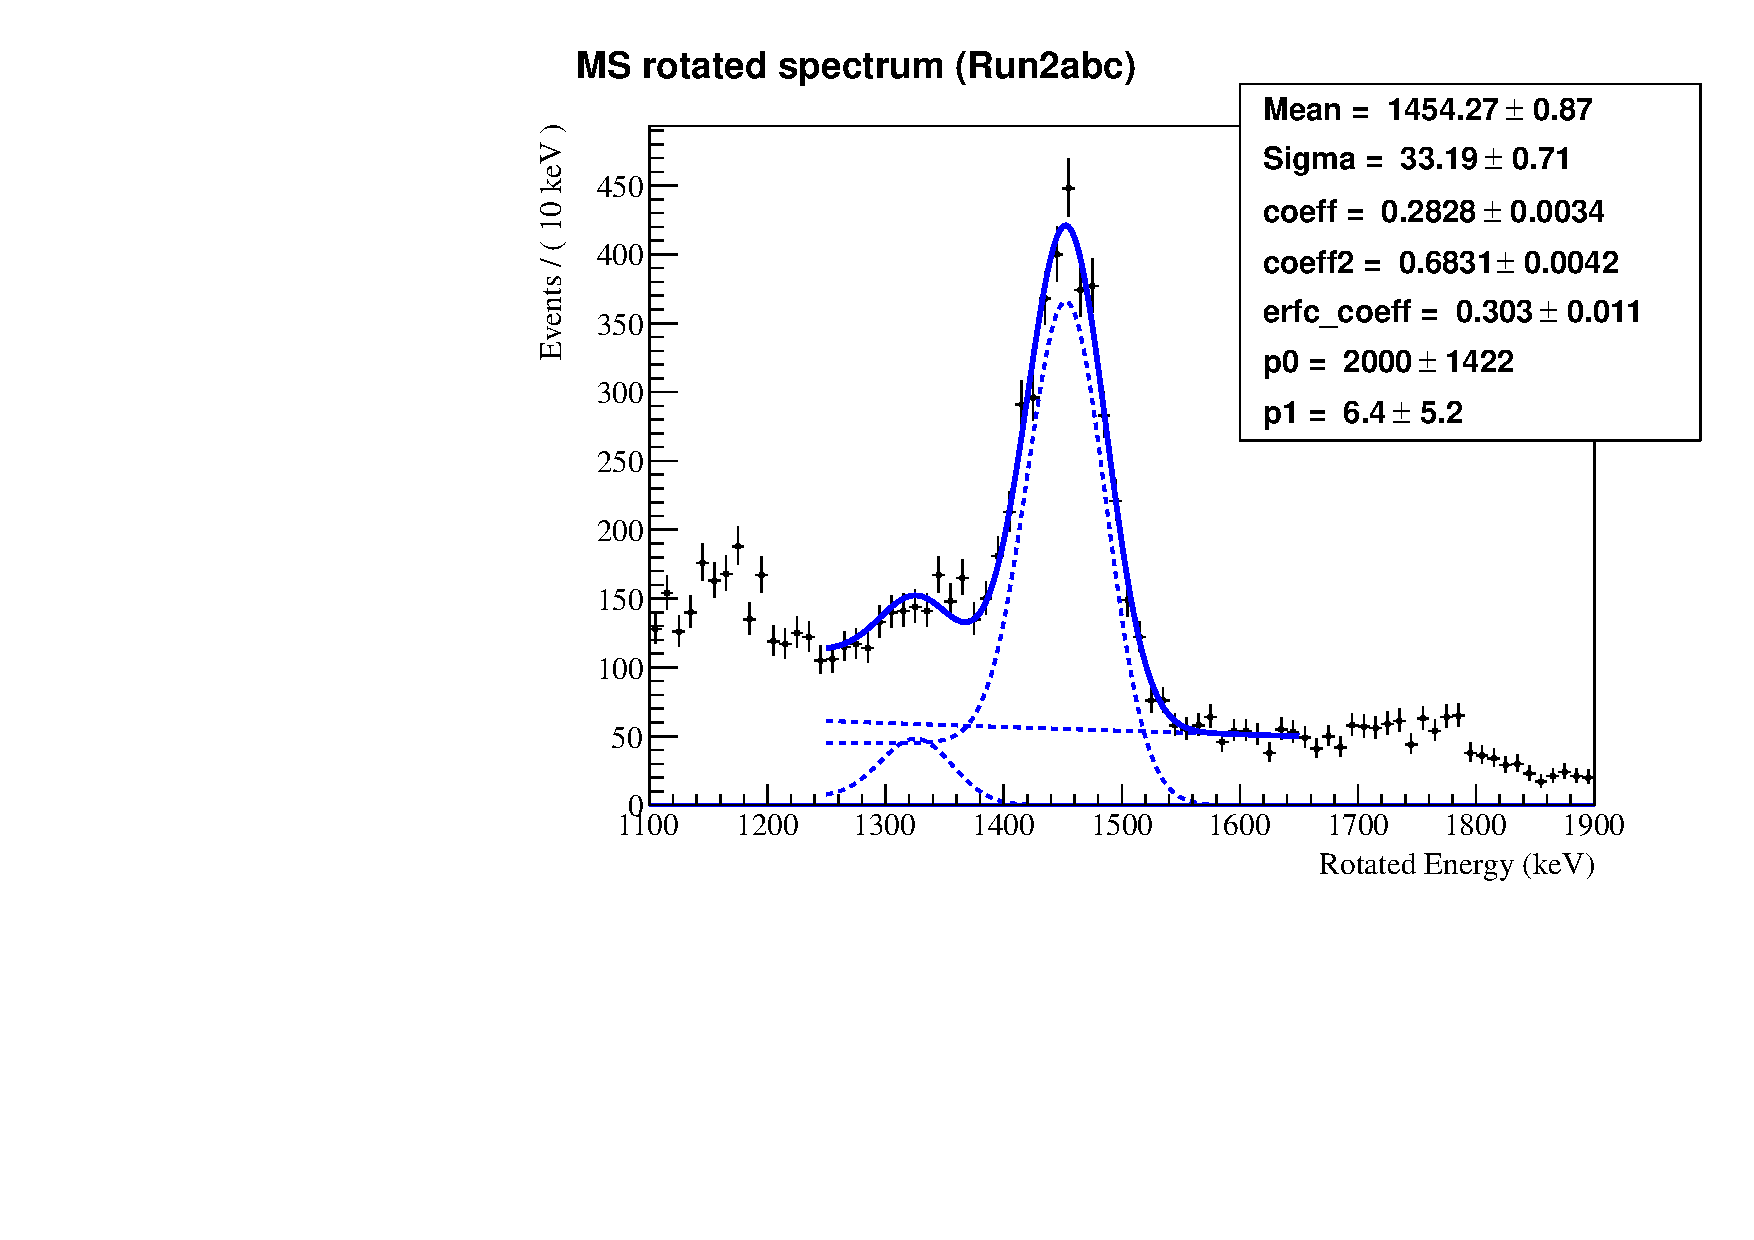
\includegraphics[keepaspectratio=true,width=.49\textwidth]{EXO_Workspace_Run2abc_K40_ms_1250keVto1650keV.pdf}
\end{center}
\renewcommand{\baselinestretch}{1}
\small\normalsize
\begin{quote}
\caption{The low-background potassium peak at $1461$ keV is used as a cross-check on the single-site (left) and multi-site (right) energy calibrations.  Fits also include the nearby $1332$-keV cobalt peak~\cite{EnergyDocumentRun2ab}.}
\label{fig:PotassiumPeakCheck}
\end{quote}
\end{figure}
\renewcommand{\baselinestretch}{2}
\small\normalsize

The other gamma line which has been used as a cross-check is the $1461$-keV $^{40}$K gamma line.  $^{40}$K is expected to occur in the copper of the TPC at some low level, and this gamma line is readily visible in the multi-site spectrum of low-background data.  The improved energy resolution of denoised data allows us to also identify the $^{40}$K single-site peak over the $\beta\beta 2\nu$ background, which was not previously possible.  These peaks are shown in figure~\ref{fig:PotassiumPeakCheck}.

\begin{figure}
\begin{center}
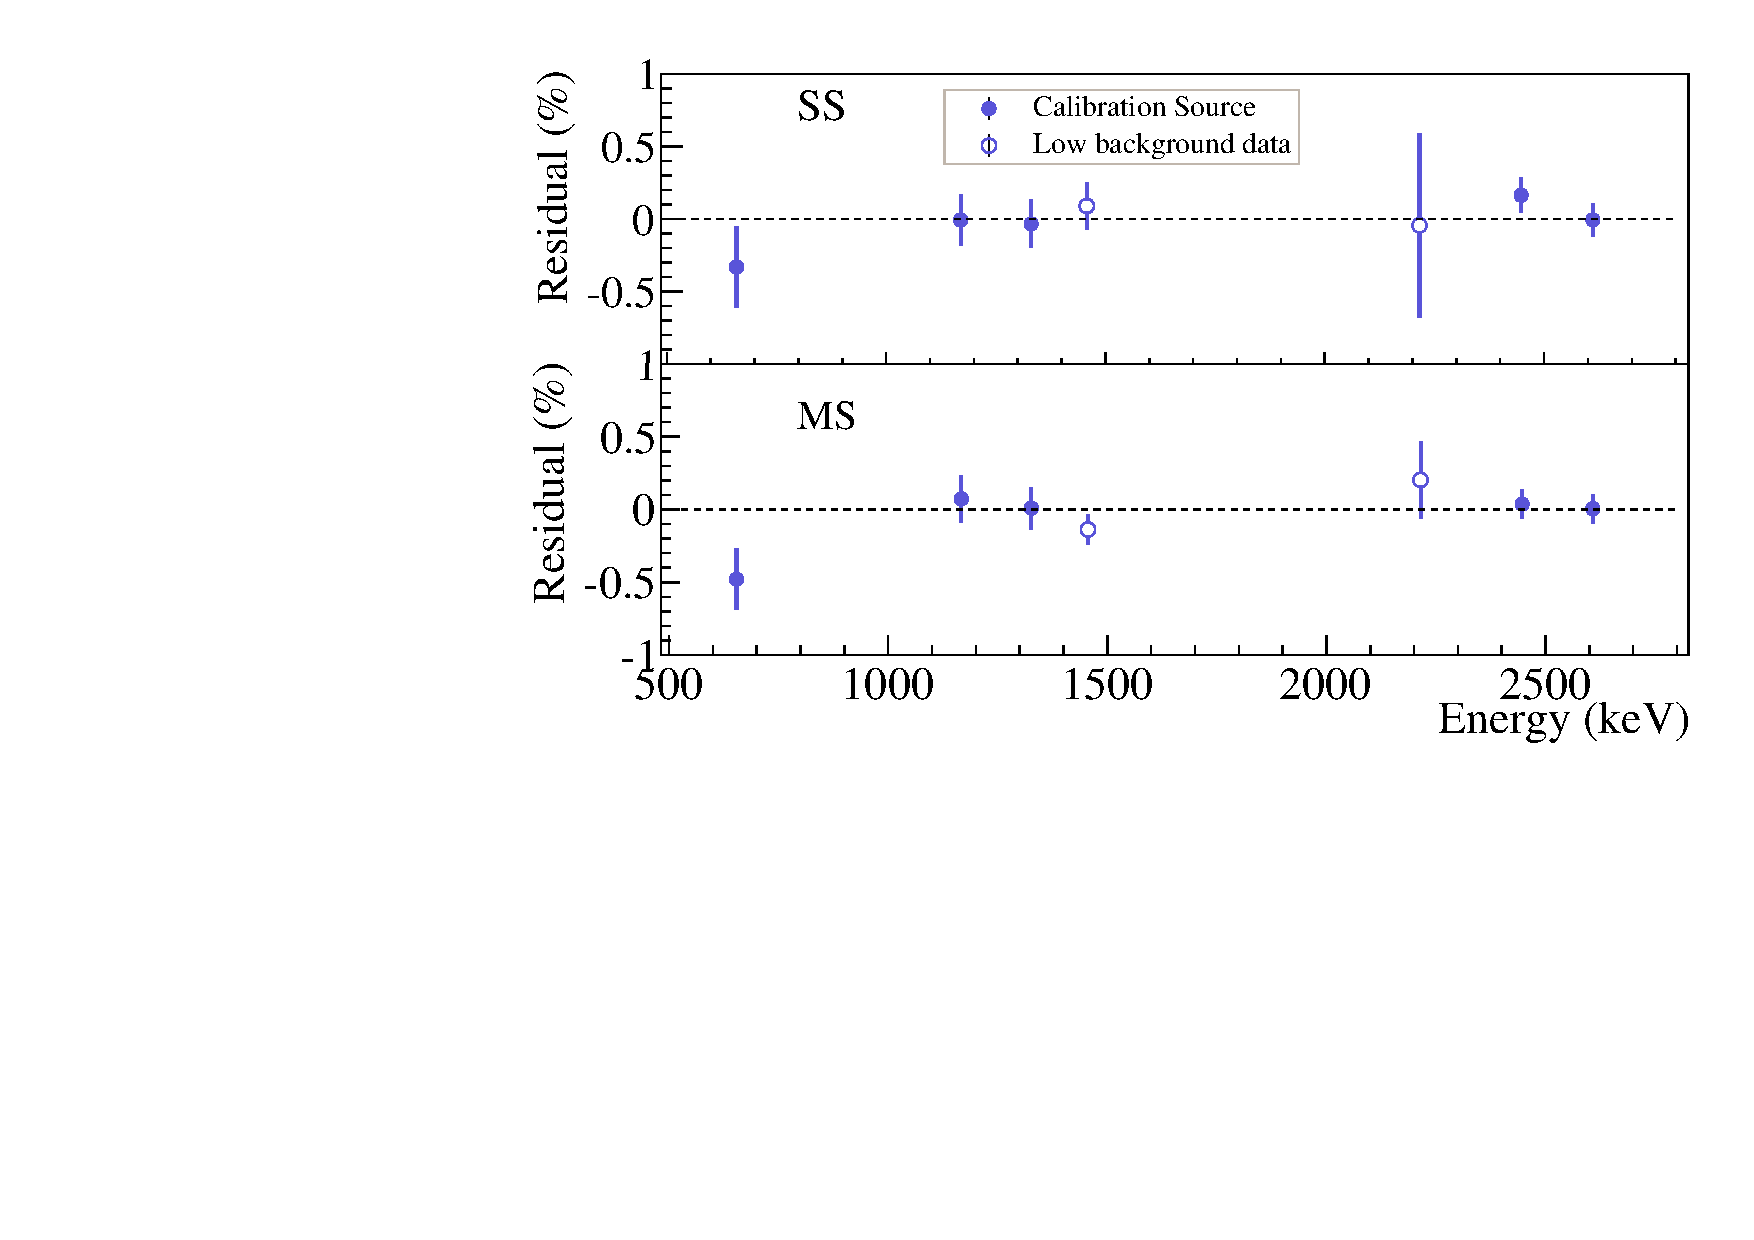
\includegraphics[keepaspectratio=true,width=\textwidth]{residual_bb0n_denoised.pdf}
\end{center}
\renewcommand{\baselinestretch}{1}
\small\normalsize
\begin{quote}
\caption{The residuals between calibrated and true peak positions for all sources is compared.  Calibrations were obtained from the $^{137}$Cs, $^{60}$Co, and $^{232}$Th peaks at 662, 1173, 1332, and 2615 keV.  The peak from $^{226}$Ra at 2448 keV is also shown, but was not used for calibration.  Low-background calibration lines are neutron capture on hydrogen (2200 keV) and $^{40}$K (1461 keV).  Figure from~\cite{EnergyDocumentRun2ab}.}
\label{fig:CalibResidualsForManySources}
\end{quote}
\end{figure}
\renewcommand{\baselinestretch}{2}
\small\normalsize

The result from combining all of these calibration points is shown in figure~\ref{fig:CalibResidualsForManySources}.  We can see that all sources agree well with the calibration, indicating that the calibration derived from thorium and cobalt extends well to the other calibration sources and captures time-dependent calibration information well.  (With 14 independent measurements under consideration, the $2\sigma$ discrepancy of the 662 keV cesium multi-site peak position should not be considered significant.)

\begin{figure}
\begin{center}
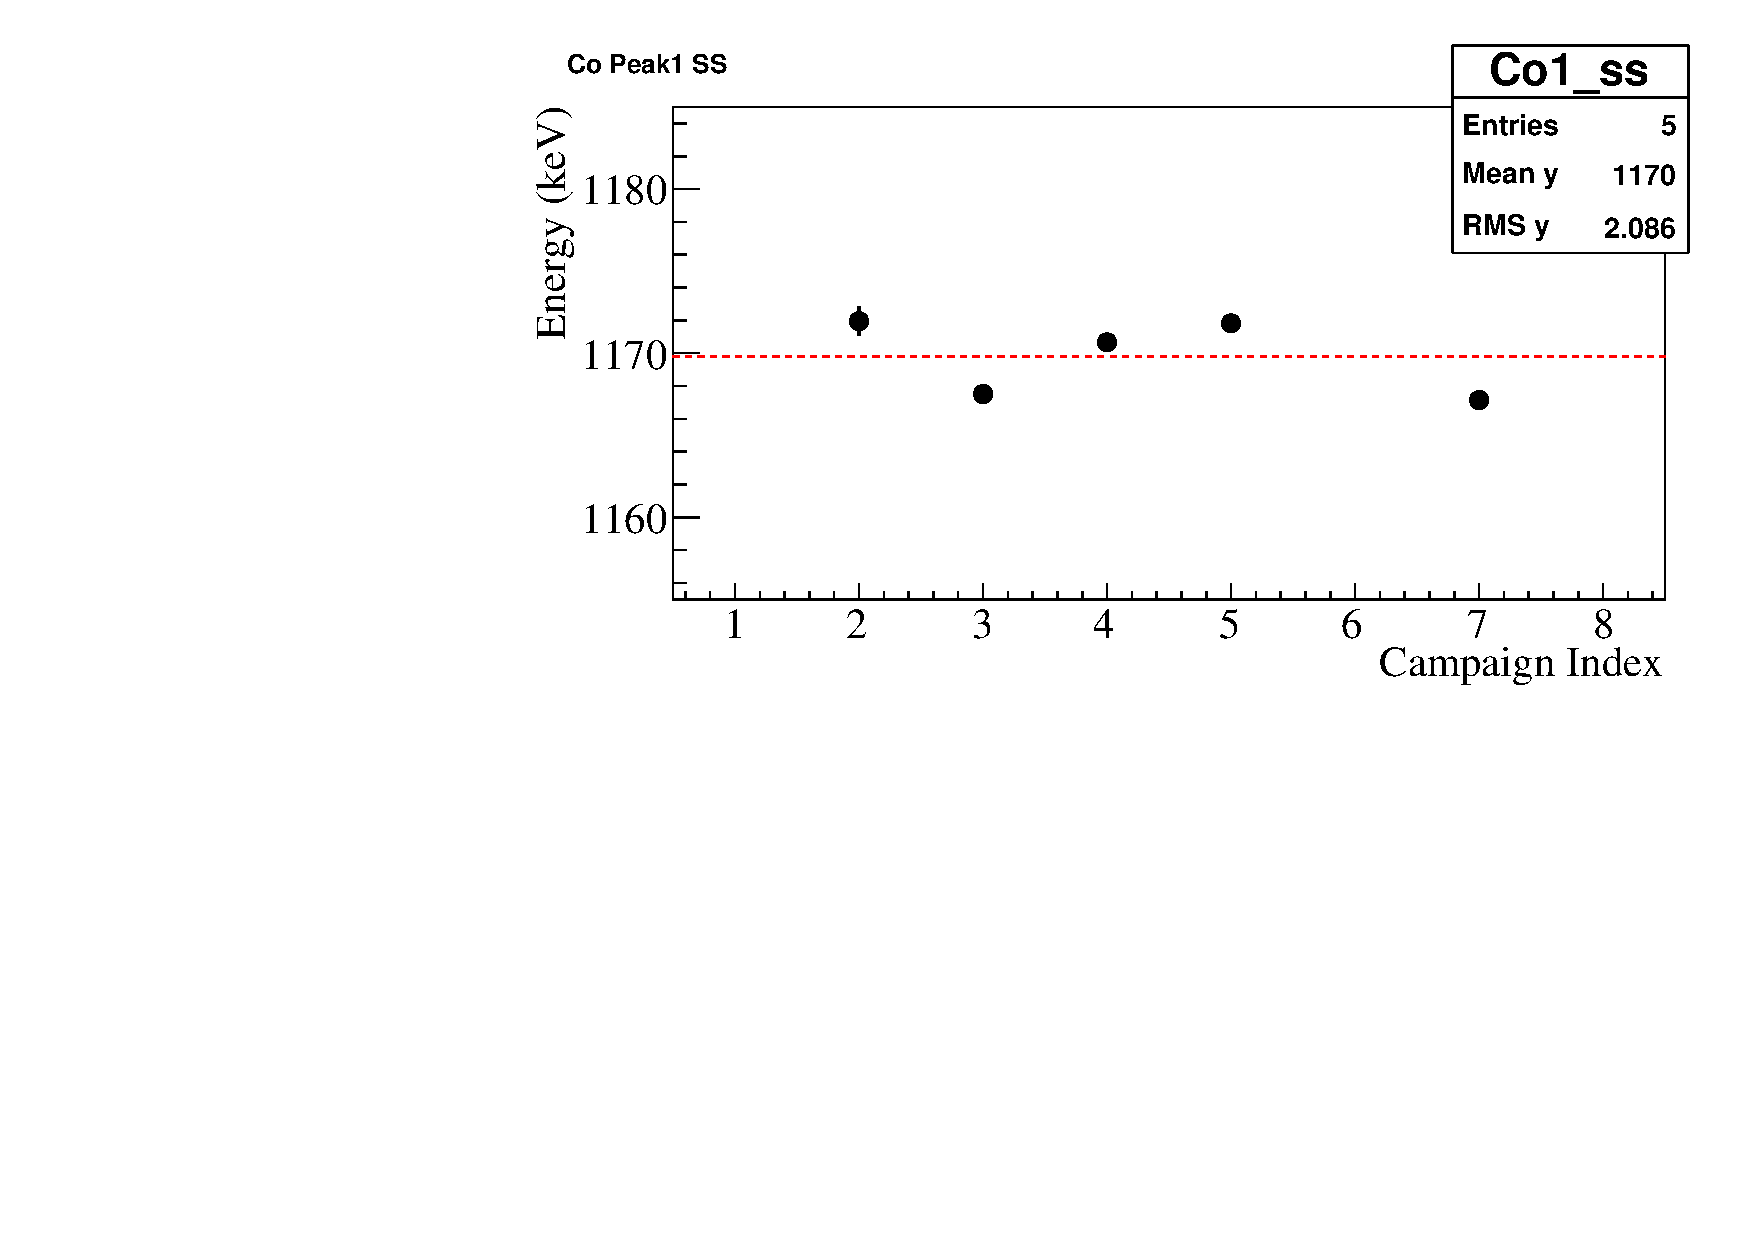
\includegraphics[keepaspectratio=true,width=.49\textwidth]{Co1_ss.pdf}
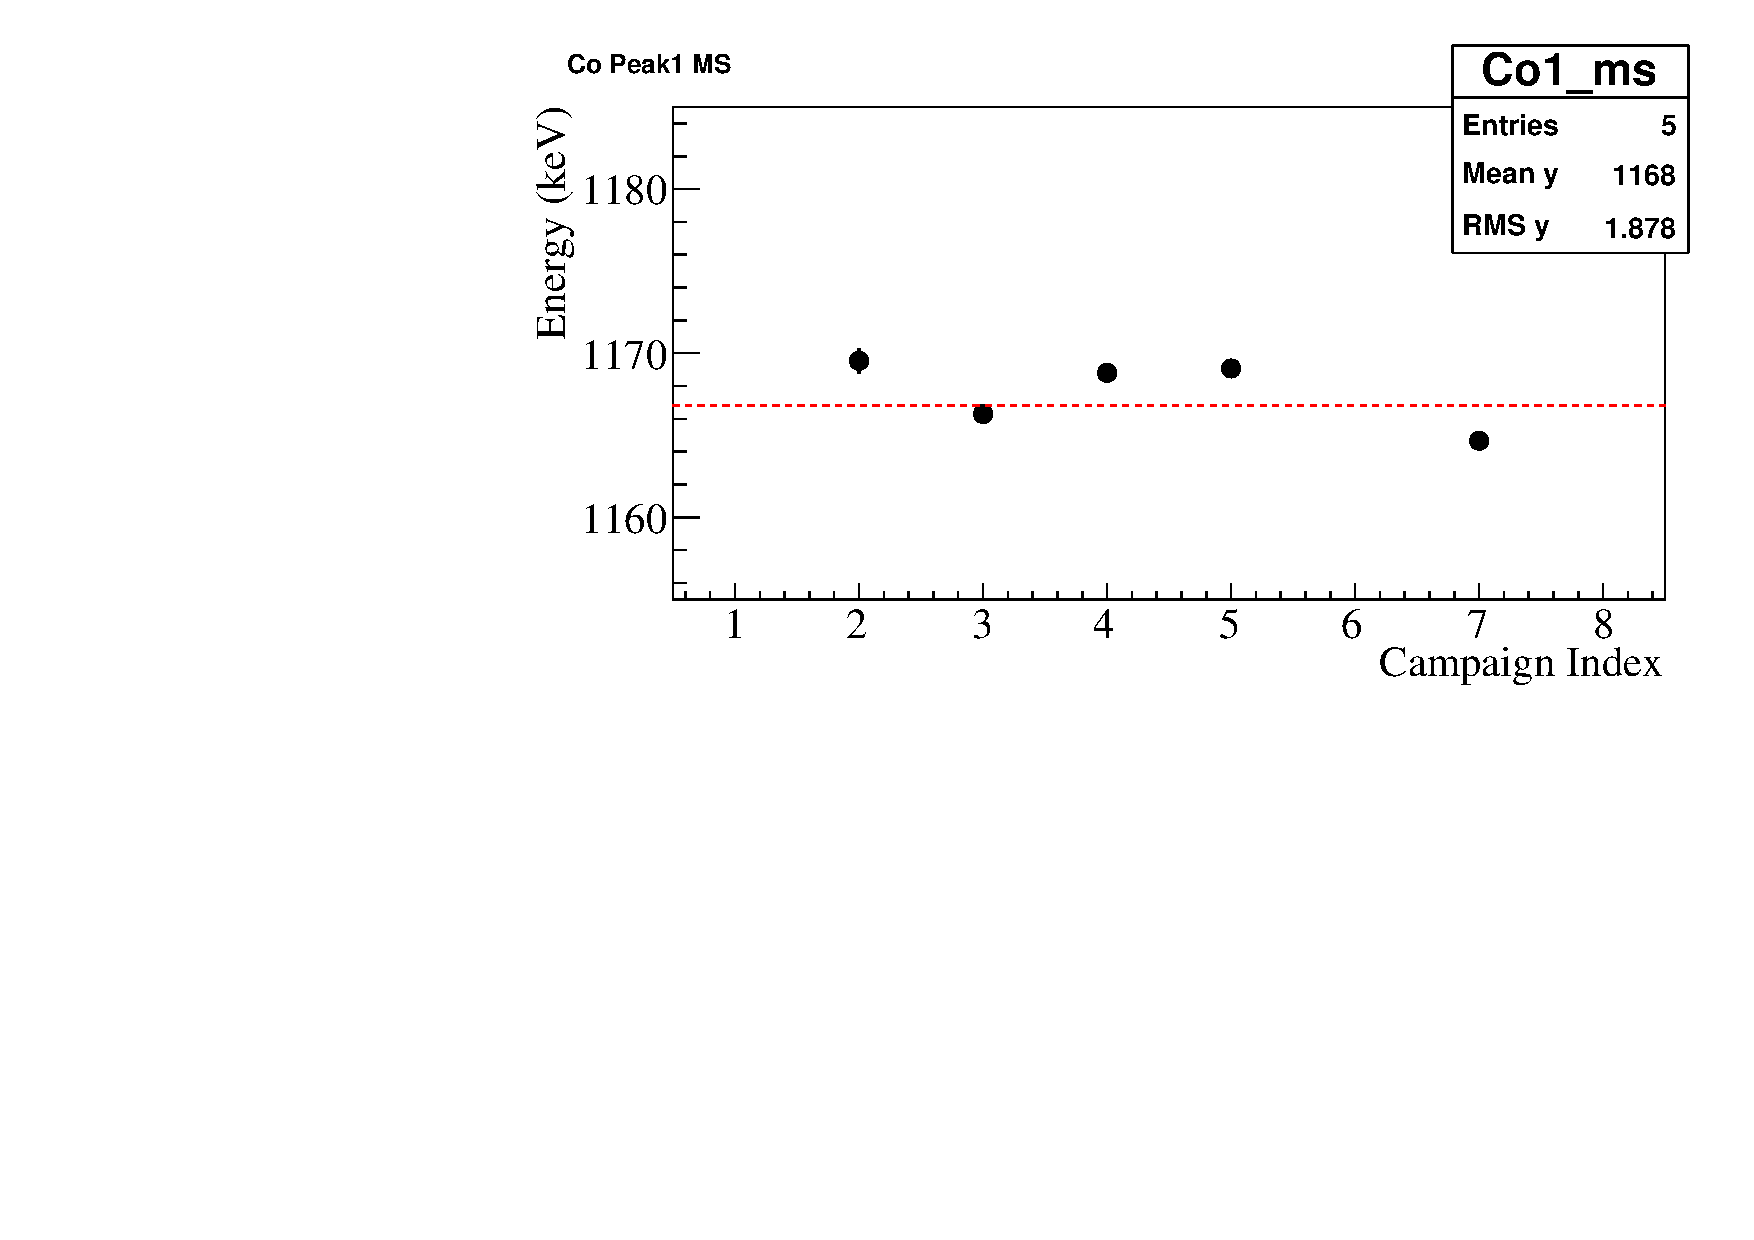
\includegraphics[keepaspectratio=true,width=.49\textwidth]{Co1_ms.pdf}
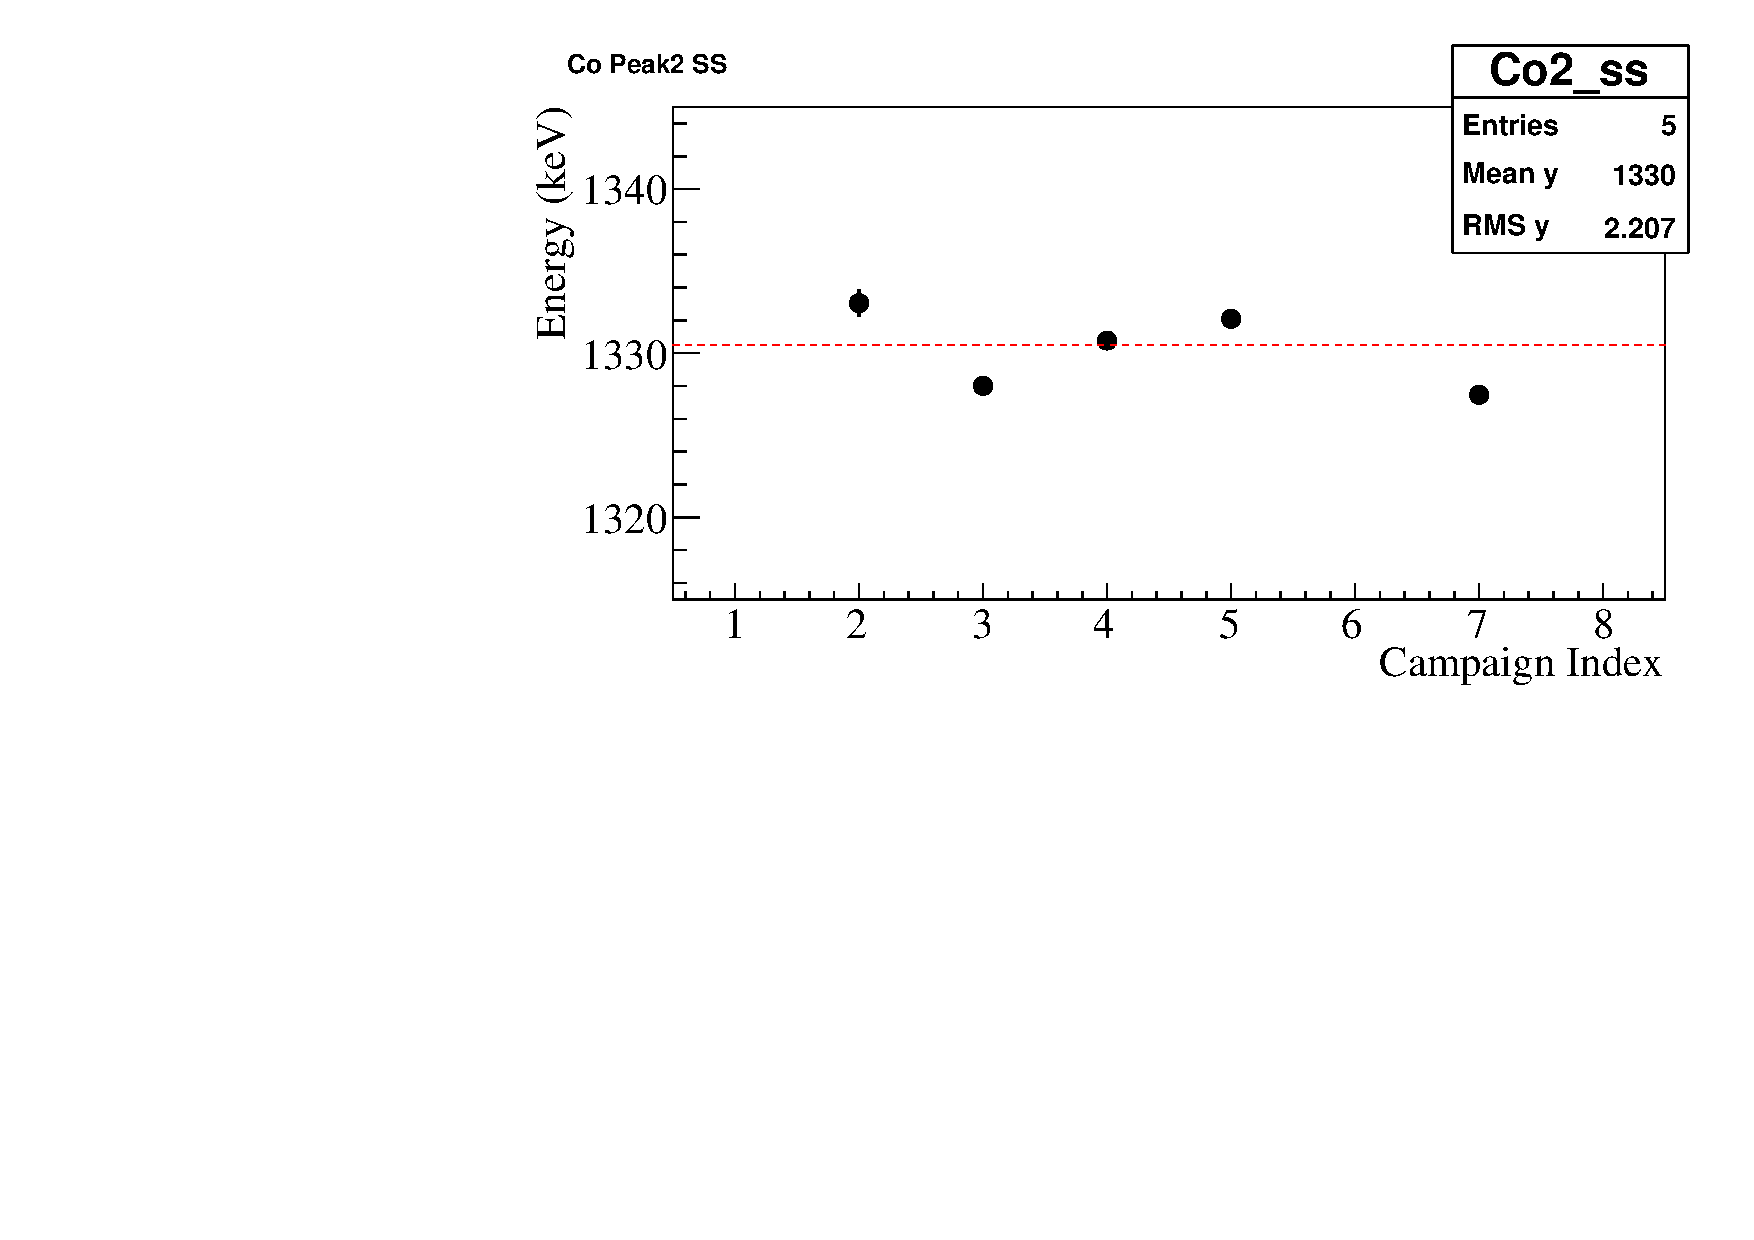
\includegraphics[keepaspectratio=true,width=.49\textwidth]{Co2_ss.pdf}
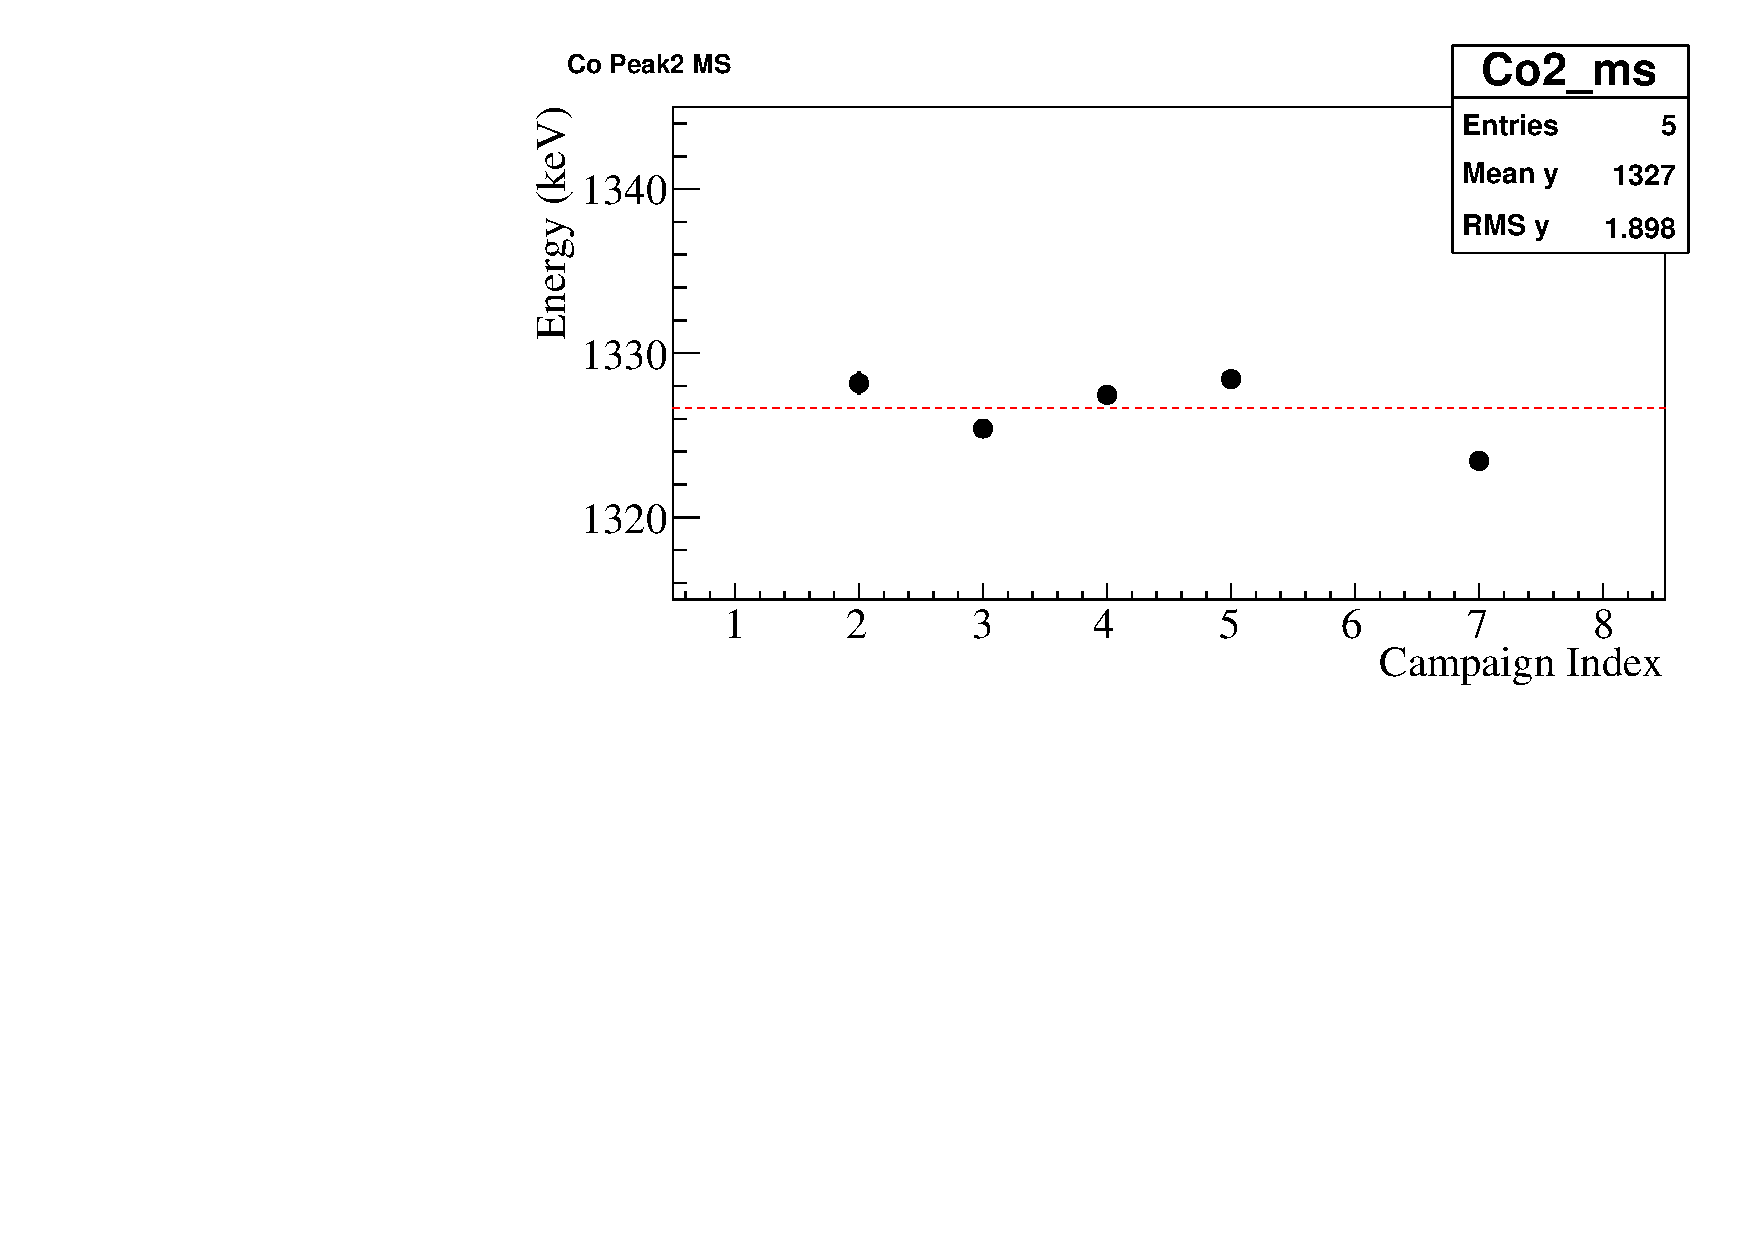
\includegraphics[keepaspectratio=true,width=.49\textwidth]{Co2_ms.pdf}
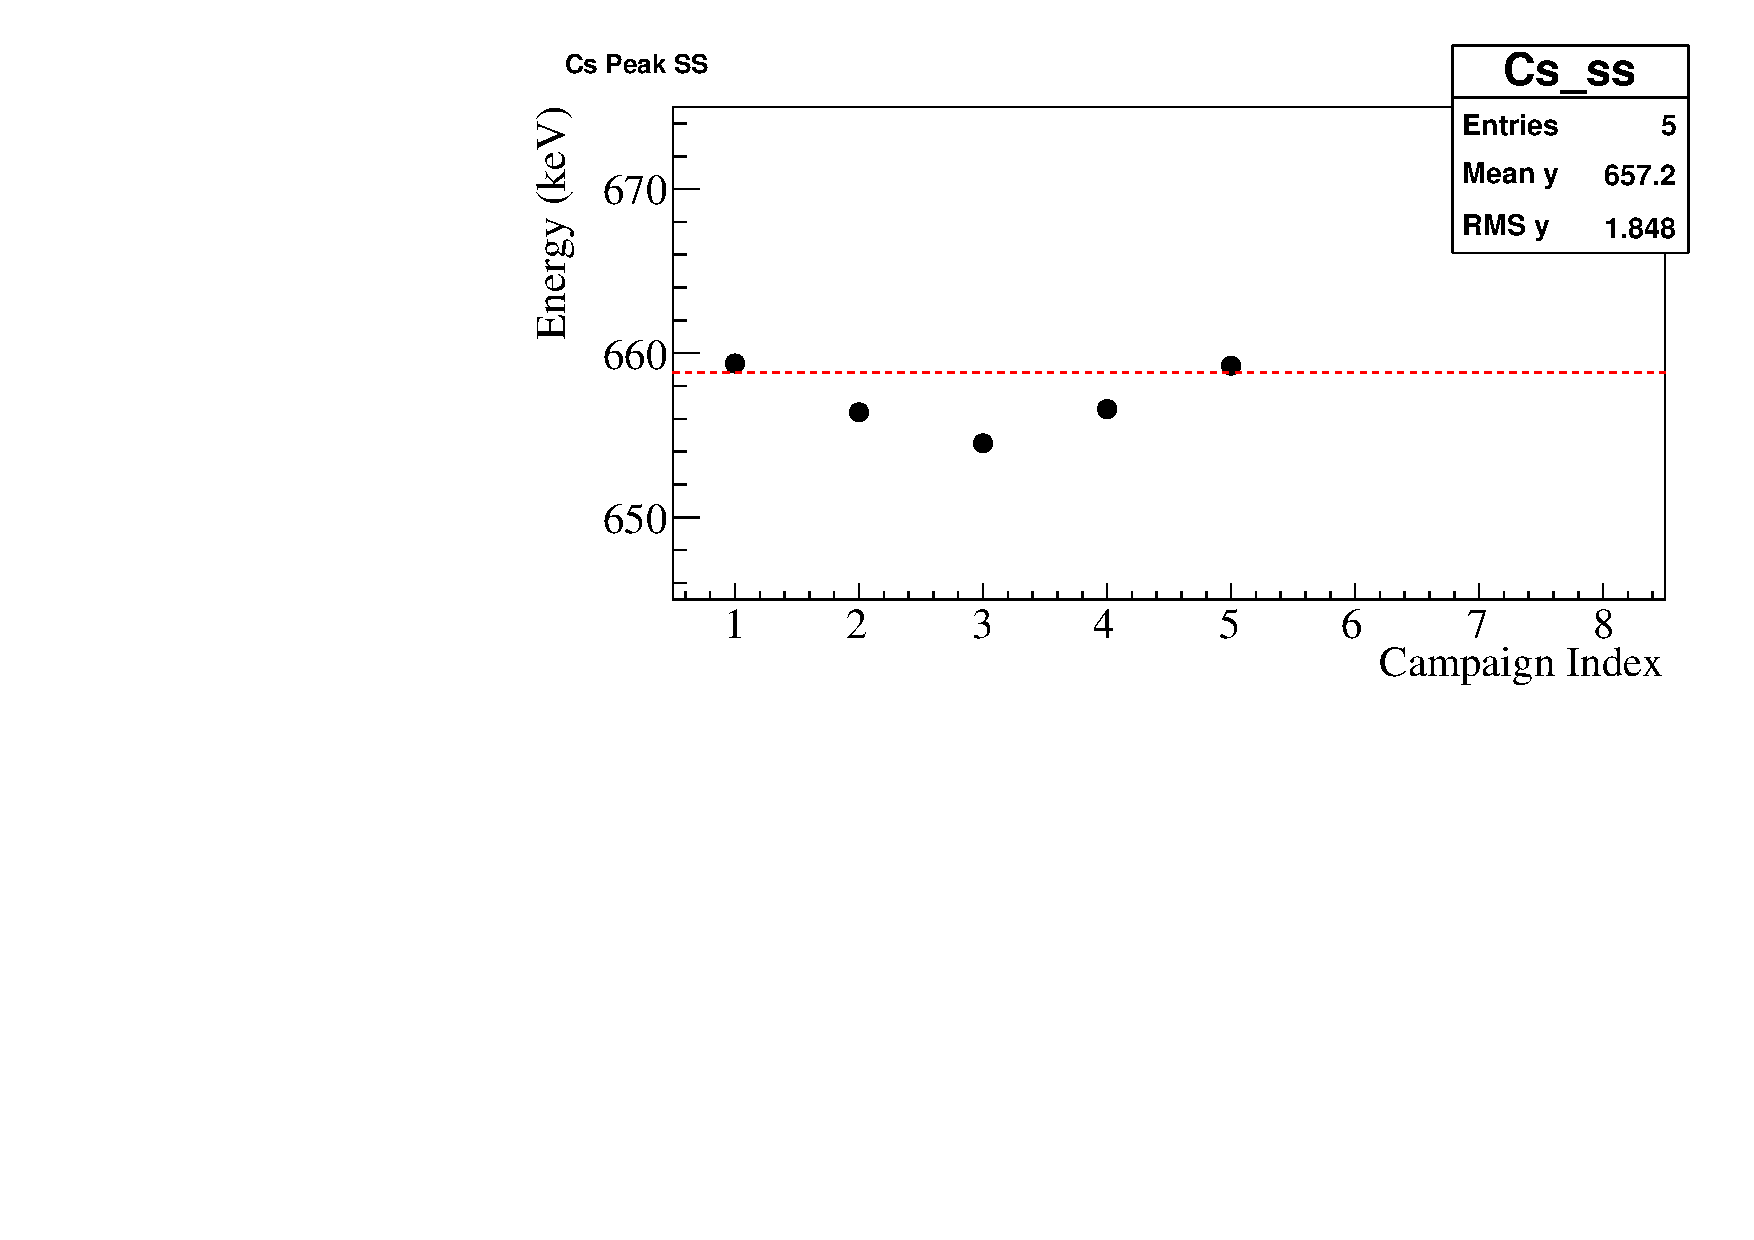
\includegraphics[keepaspectratio=true,width=.49\textwidth]{Cs_ss.pdf}
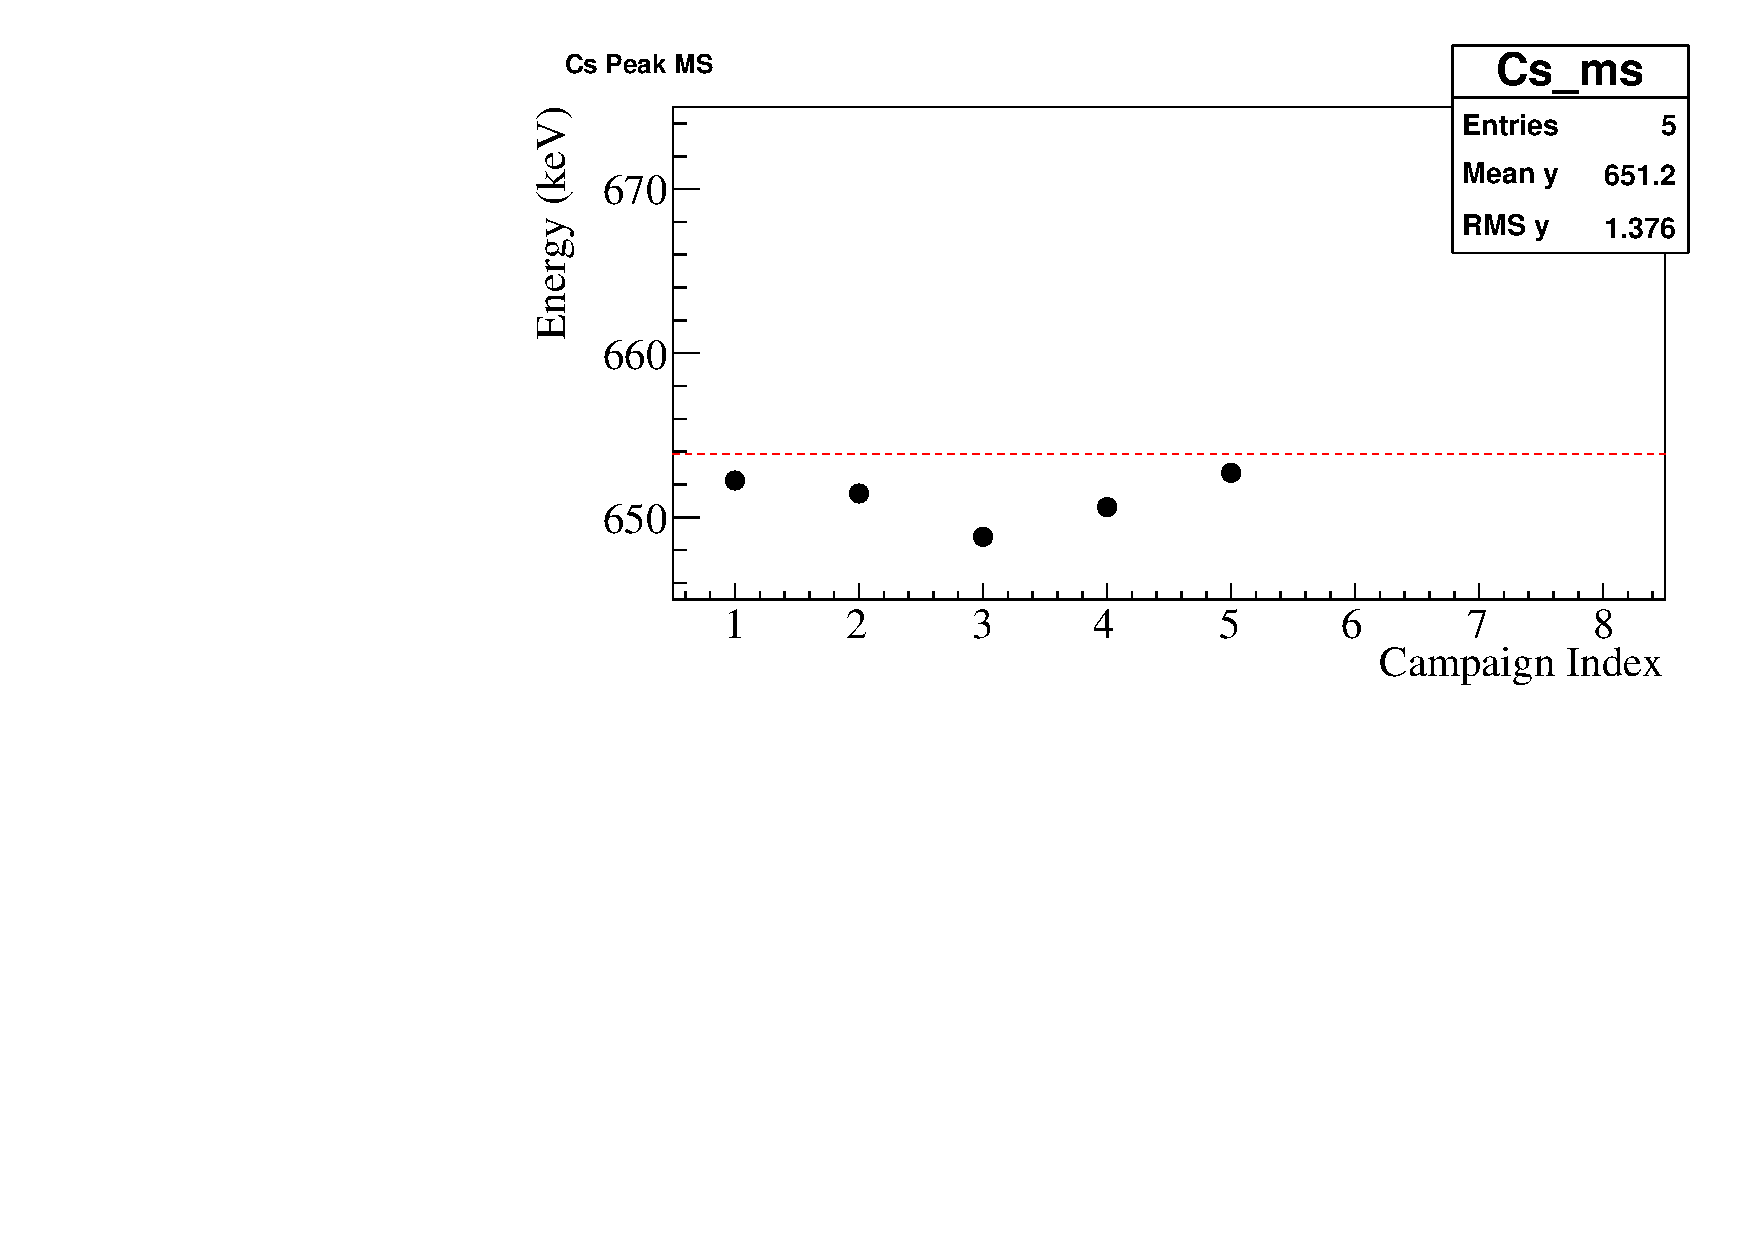
\includegraphics[keepaspectratio=true,width=.49\textwidth]{Cs_ms.pdf}
\end{center}
\renewcommand{\baselinestretch}{1}
\small\normalsize
\begin{quote}
\caption{Time-dependence of the peak positions from all calibration campaigns.  Error bars, when not visible, are smaller than the circle.  Top row is the $^{60}$Co peak at 1173 keV; middle row is the $^{60}$Co peak at 1332 keV; bottom row is the $^{137}$Cs peak at 662 keV.  Thorium is not included because it is used to measure the time-dependence of the peak positions, so it is necessarily calibrated to a time-independent value.  Figure from~\cite{EnergyDocumentRun2ab}.}
\label{fig:CalibPeakPosTimeDep}
\end{quote}
\end{figure}
\renewcommand{\baselinestretch}{2}
\small\normalsize

We also use the calibration source peak positions to check that the calibrated peak positions remains constant over time.  This is automatic for the thorium peak position at 2615 keV because that peak is used to measure the time-dependence of the calibration.  However, if we see that the cesium calibrated peak position changes over time, for example, then this would indicate that the time-dependent calibration parameters $\theta(t)$ and $E^{th}_{rot}(t)$ of equation~\ref{eqn:EnergyCalibrationParametrization} are inadequate to describe the time-dependent behavior of the detector.  The peak positions of cesium and cobalt are shown in figure~\ref{fig:CalibPeakPosTimeDep}.  There we can see that indeed the peak positions of these sources do vary by more than their statistical error bars.  In this analysis, the variations in peak position are treated as variations in the spectral shapes of sources and incorporated as a systematic effect~\cite{EnergyDocumentRun2ab,FittingDocument}.

\begin{figure}
\begin{center}
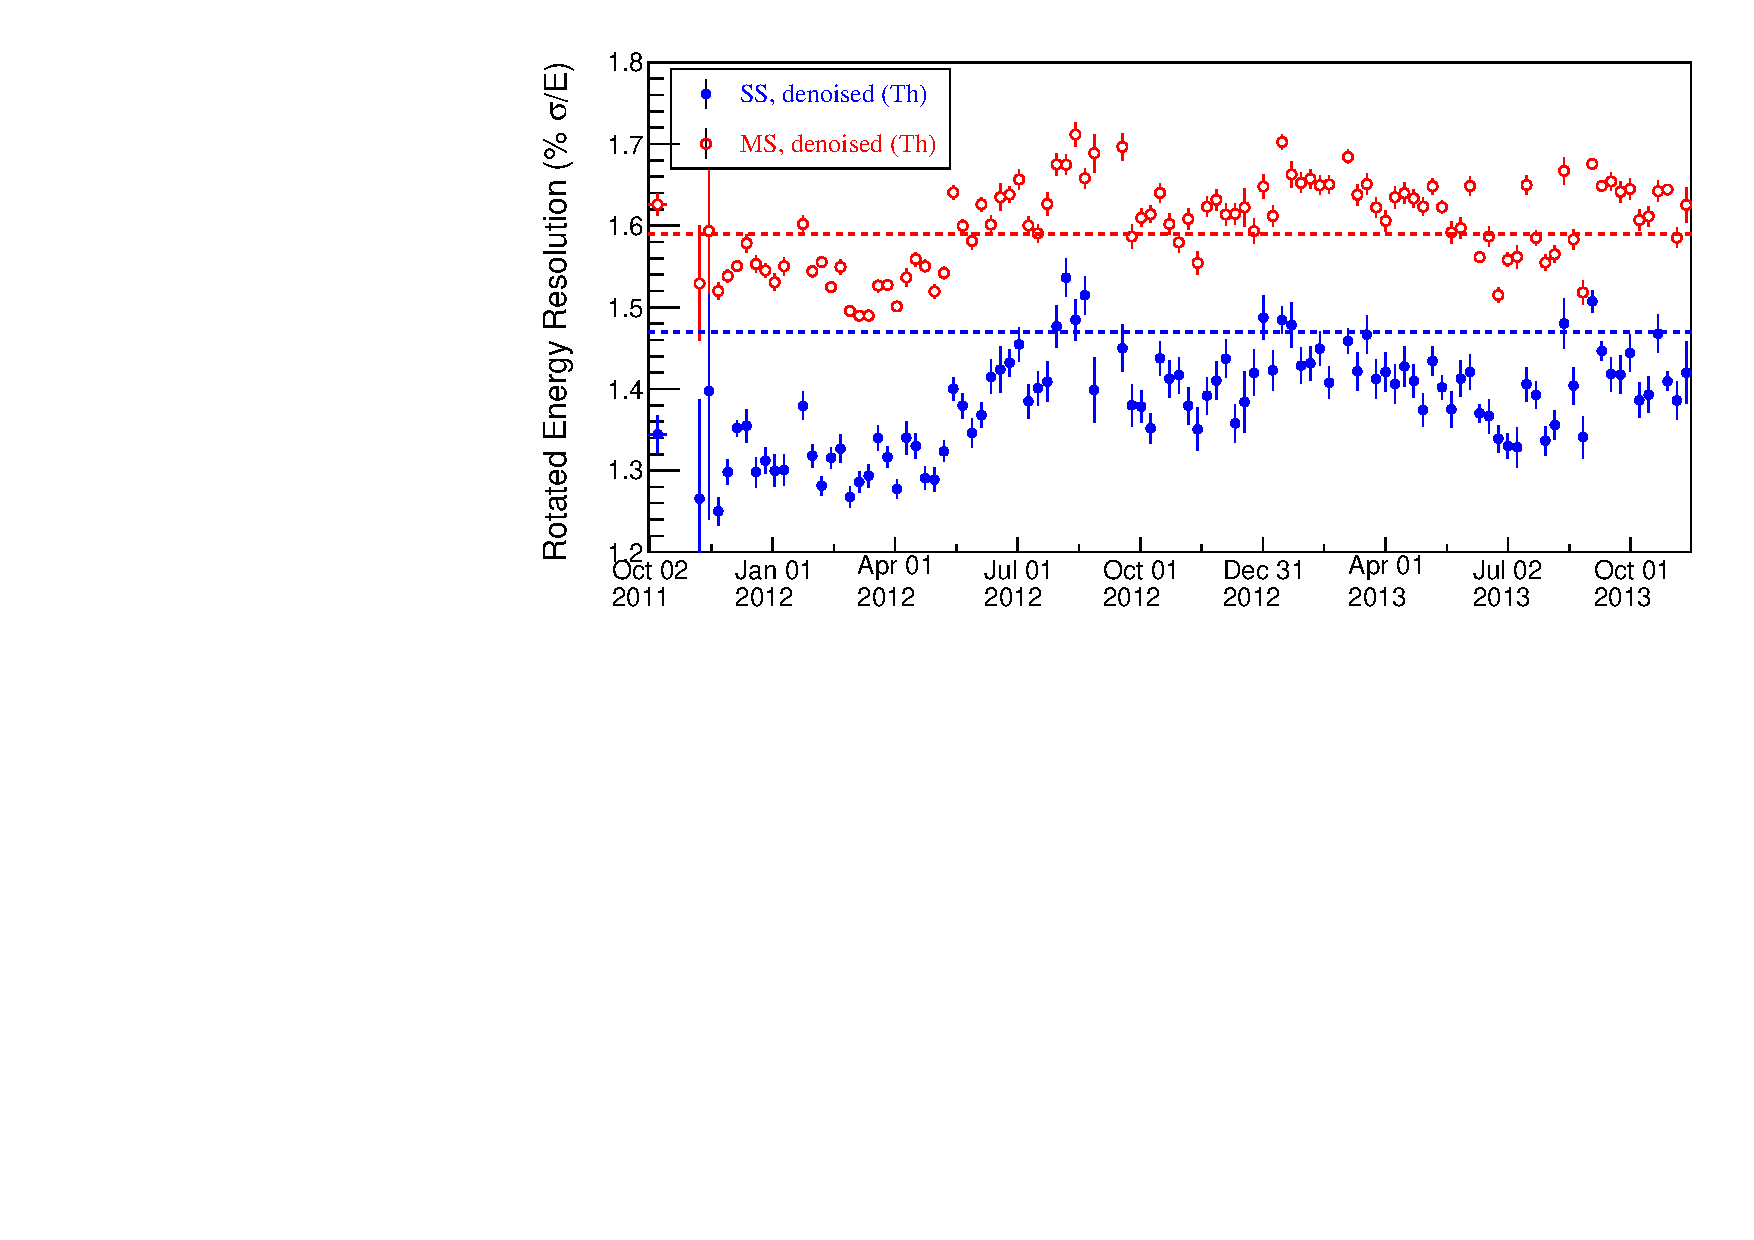
\includegraphics[keepaspectratio=true,width=\textwidth]{ThDenoisedResVsTime.pdf}
\end{center}
\renewcommand{\baselinestretch}{1}
\small\normalsize
\begin{quote}
\caption{Time-dependence of the energy resolution at the $^{208}$Tl 2615 keV gamma line.  Single-site (blue) and multi-site (red) energy resolutions are shown.  The time-averaged energy resolutions (1.47\% $\sigma/E$ for single-site, 1.59\% $\sigma/E$ for multi-site, both at 2615 keV) are shown in blue and red dashed lines, respectively.  Data provided by Liangjian Wen.}
\label{fig:ThoriumDenoisedResVsTime}
\end{quote}
\end{figure}
\renewcommand{\baselinestretch}{2}
\small\normalsize

Lastly, it is necessary to study the energy resolution as a time-dependent quantity.  This is only done with the thorium source because of the regularity of thorium runs that have been taken.  The time-dependent resolution observed from thorium calibration runs is shown in figure~\ref{fig:ThoriumDenoisedResVsTime}.  We can see that there are statistically significant variations in resolution over time; these, combined with the time-varying peak positions shown in figure~\ref{fig:CalibPeakPosTimeDep}, lead to a weakened time-averaged energy resolution which accounts for the smearing of low-background peaks over the span of our dataset~\cite{AverageEnergyResolutionDocument}.

The cross-checks described here identify features of the energy response which are not fully calibrated; these are treated as smearing effects over time and lead to a weakening of our time-averaged energy resolution.  Future work will be targeted toward understanding the peak position variations with event position shown in figure~\ref{fig:ResidualLightZBias} and with time shown in figures~\ref{fig:CalibPeakPosTimeDep} and \ref{fig:ThoriumDenoisedResVsTime}.  Resolving these issues should lead to further improvements in the time-averaged resolution of EXO-200 in later analyses.

\section{Fitting}\label{sec:ResultFitting}

After the energy calibrations have been performed, it is possible to produce a set of data with calibrated energy measurements.  This section describes the selection of usable events from this dataset, the creation of corresponding background probability distribution functions (PDFs), the fitting of data to extract the best-fit number of $\beta\beta 0\nu$ events in the dataset, and the association of errors with that number.  Results from the current analysis are demonstrated along the way, leading to a limit for $\beta\beta 0\nu$ decay.

\begin{figure}
\begin{center}
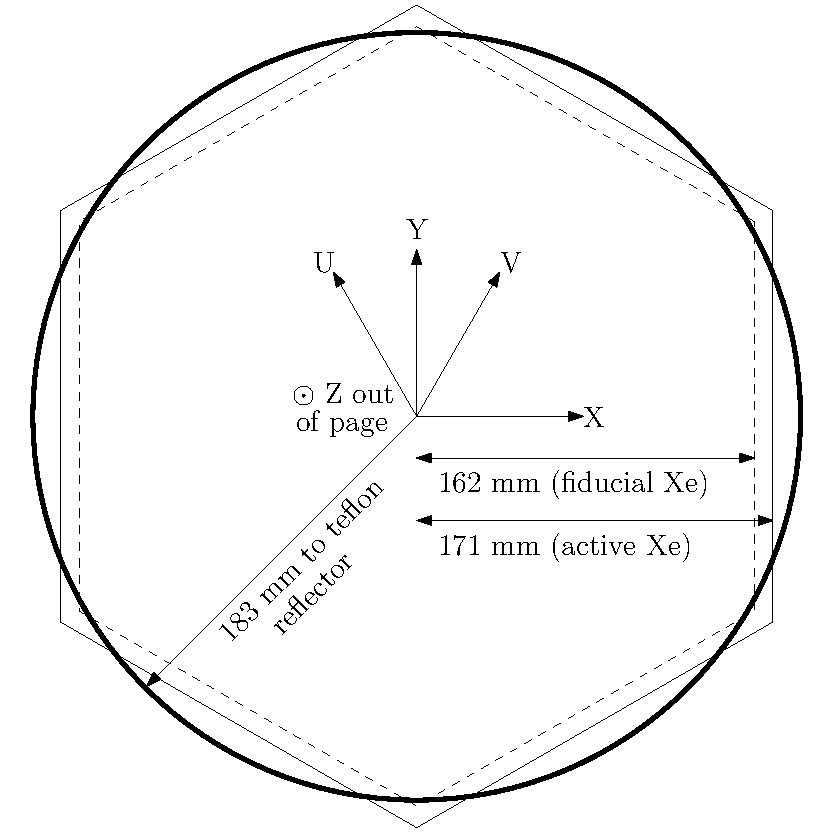
\includegraphics[keepaspectratio=true,width=\textwidth]{FidVolDiagram_Dissertation.pdf}
\end{center}
\renewcommand{\baselinestretch}{1}
\small\normalsize
\begin{quote}
\caption{Here the X-Y orthogonal coordinates are shown along with the U-V coordinates that run orthogonal to the wire planes.  The X-Y fiducial cuts applied to the data (dashed hexagon) do not include the entire active volume (solid hexagon); for the $\beta\beta 0\nu$ search we find that aggressive fiducial cuts optimize our sensitivity, so very little active xenon is left unused.}
\label{fig:FidVolDiagram}
\end{quote}
\end{figure}
\renewcommand{\baselinestretch}{2}
\small\normalsize

\begin{figure}
\begin{center}
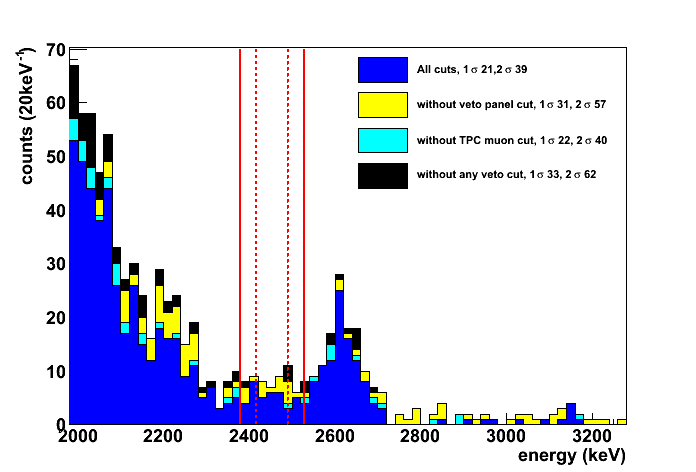
\includegraphics[keepaspectratio=true,width=\textwidth]{SS_Spectrum_noVetoCuts.png}
\end{center}
\renewcommand{\baselinestretch}{1}
\small\normalsize
\begin{quote}
\caption{Vetoing events coincident with muons can reduce our $1\sigma$ and $2\sigma$ event counts.  Figure provided by David Auty.}
\label{fig:Spectrum_noVetoCuts}
\end{quote}
\end{figure}
\renewcommand{\baselinestretch}{2}
\small\normalsize

It is necessary to perform a number of cuts on the dataset before it is usable.  These cuts are intended to reject events which may not agree with the model used to generate background PDFs.  These cuts are:~\cite{FittingDocument}
\begin{itemize}
\item A fiducial volume cut to remove events with any energy deposits outside of a pre-defined volume.  We choose to define a fiducial volume defined in Z by $10 \text{mm} < |Z| < 182 \text{mm}$ and in the X-Y plane as the area within a hexagon with an apothem of $162$ mm, as illustrated in figure~\ref{fig:FidVolDiagram}.  These cuts allow us to ignore regions near the detector walls or v-wire plane where the electric fields may not behave as expected.  They also ensure that beta or alpha backgrounds from the walls of the detector do not penetrate into our fiducial volume, allowing us to simplify the set of backgrounds modeled and included in fits.
\item A ``diagonal'' cut to remove events with excessive scintillation relative to ionization.  Alpha decays produce a light-to-charge ratio much higher than beta and gamma decays, as described in section~\ref{sec:DetectorActiveBackgroundRejection}, so excluding events with excessive light permits us to neglect alpha-decay backgrounds dissolved in the xenon.  Events with excessive light can also be caused by decays outside of our active xenon, where charge is not collected efficiently; these events will be difficult to calibrate, and should not be included.  Both are excluded by a cut on the light-to-charge ratio, as shown in figure~\ref{fig:LiangjianAnticorrelatedEnergy}.
\item A coincidence cut to remove events occurring near in time to a passing muon.  Muons and their spallation products can produce a wide range of backgrounds which is difficult to model; most of these backgrounds are quite short-lived, so a coincidence cut can provide an effective means of reducing them.  Currently we cut all events occurring within one minute of a muon observed passing directly through the TPC and within $25$ ms after a muon observed passing through the veto panels.  Furthermore, events which occur within one second of each other are both cut based on the expectation that the events were probably correlated and therefore more likely to be some form of background.  Figure~\ref{fig:Spectrum_noVetoCuts} demonstrates the significant reduction in data rate which is achieved by applying this coincidence cut.
\end{itemize}
The fiducial volume identified above corresponds to a fiducial $^{136}$Xe mass of 76.3 kg; for our livetime of $477.60 \pm 0.01$ days identified at the beginning of the chapter, the dataset has a combined $^{136}$Xe exposure of 99.8 kg-years~\cite{NewEXObb0nPaper_2014}.

Probability distribution functions (PDFs) must also be formed from Monte Carlo data which reflects the spectrum expected from different sources.  We have discussed the simulation of these datasets in section~\ref{sec:ResultSimulation}, and noted that the simulations are sufficiently realistic that they are reconstructed in exactly the same way as data.  However, we cannot hope to measure energy in simulation and data the same way because the scintillation pulse amplitudes are not simulated realistically.

Instead, energy is taken directly from simulation and smeared by the energy resolution function which has been measured from data.  Smearing is performed by first producing a binned perfect-resolution PDF which models perfect energy resolution, and then looping over the bins of the perfect-resolution PDF and smearing each bin by a Gaussian function with width equal to the absolute resolution at that energy~\cite{FittingDocument}.

Fits are then performed using the profile-likelihood method, as described in~\cite{ProfileLikelihood}.  An energy window of 980-9800 keV is used; this window is chosen to avoid lower-energy parts of the spectrum where pdf shape agreement is poor~\cite{NewEXObb0nPaper_2014}.  Each data point is assigned a likelihood $\text{PDF}(x)$ equal to the evaluation of the normalized PDF at that point; the test statistic of interest is the negative log-likelihood (NLL), defined by:
\begin{equation}
\text{NLL} = -\sum_i ln\left[\text{PDF}(x_i)\right] + \text{constraints}.
\end{equation}
Constraints are Gaussian penalty terms applied to parameters whose value is constrained by independent studies external to the fit.  The best fit is the one which minimizes the NLL.  Fit errors on parameters are extracted by observing how the NLL changes when those parameters are forced away from their best-fit values; $1\sigma$ limits are placed where the NLL changes by 0.5 units from its best-fit value, and $90\%$ limits are placed where the NLL changes by 1.35 units from its best-fit value.  In cases where the best-fit value of a parameter is near its boundary, these errors may not provide a good estimate of the true confidence interval or limits, so when this situation occurs for a parameter of significant interest (specifically, the rate of $\beta\beta 0\nu$, which fits near to zero) we can verify that the confidence limit is not overstated using toy Monte Carlo studies~\cite{FittingDocument}.

The fits make use of three observables.  The first, event energy, has been discussed at length in section~\ref{sec:RotatedEnergyCalibration}.  The second is the event classification as single-site or multi-site; we define an event as single-site if reconstruction located only one cluster, and that cluster deposited charge on no more than two u-wire channels~\cite{FittingDocument}.  This choice of definition ensures that a dense cloud of charge which approaches the anode at a midpoint between two u-wire channels and gets split apart will still be counted as single-site.

The third observable is called standoff distance, and it attempts to capture the nearness of an event to the TPC walls.  Most backgrounds are external, and can be expected to deposit energy preferentially near the walls of the TPC; by contrast, $\beta\beta 0\nu$ and $\beta\beta 2\nu$ decay come from the xenon, and should be distributed uniformly through the detector.  We define the standoff distance to be the shortest distance between some deposit cluster and either the v-wire planes or the teflon walls.  Ideally, it would be possible to capture finer position information by using all three position coordinates as observables; however, in practice it is difficult to construct a PDF with sufficient statistics in so many dimensions, so the standoff observable has been constructed to capture the most interesting distances in a single observable.  The exact definition is not too important provided it is modeled properly by the simulation; figure~\ref{fig:RaSourceMCComparison} demonstrates that standoff distance is simulated well for all but the smallest values (closest to the TPC walls or anode), and this is accounted for as a shape systematic~\cite{FittingDocument}.

Fit parameters include the number of counts observed from each PDF and the fraction of counts from each PDF which populate the single-site spectrum; the latter is constrained based on the agreement between simulated and observed single-site fraction from source runs, but is allowed to float within those uncertainties.  The PDFs which are included are:
\begin{itemize}
\item $^{136}$Xe $\beta\beta 2\nu$ decay.
\item $^{136}$Xe $\beta\beta 0\nu$ decay.
\item $^{232}$Th from the TPC vessel.
\item $^{232}$Th from distant sources (HFE-7000 refrigerant or cryostat).
\item $^{238}$U from the TPC vessel.
\item $^{214}$Bi from the TPC cathode ($^{238}$U chain).
\item $^{214}$Bi from the air gap inside the lead wall ($^{238}$U chain).
\item $^{214}$Pb dissolved in active xenon ($^{238}$U chain).
\item $^{222}$Rn dissolved in inactive xenon ($^{238}$U chain).
\item $^{60}$Co from the TPC vessel.
\item $^{40}$K from the TPC vessel.
\item $^{65}$Zn from the TPC vessel.
\item $^{54}$Mn from the TPC vessel.
\item $^{137}$Xe from neutron capture on $^{136}$Xe.
\item $^{135}$Xe from neutron capture on $^{134}$Xe.
\item Various neutron captures on xenon, copper, and hydrogen.
\end{itemize}
Similar PDFs from different locations are included because the sharpness and relative intensity of peaks can be affected by intervening material.  The rate of $^{214}$Bi from the air gap is constrained by measurements of radon levels in air, and the rates of $^{214}$Bi from the TPC cathode, $^{214}$Pb dissolved in active xenon, and $^{222}$Rn dissolved in inactive xenon are jointly constrained by independent searches for $^{214}$Bi-$^{214}$Po rates.  The overall rate of neutron captures is allowed to float, but the relative intensities of the captures on xenon, copper, and hydrogen are constrained by simulation, and the single-site fraction is fixed because there are not expected to be sufficient statistics in the single-site spectrum to constrain it~\cite{FittingDocument}.

In addition to the magnitude and single-site fraction parameters of the fit, there are a few global parameters which are also allowed to float.  There is a normalization constant which is allowed to float within constraints and accounts for uncertainty in the fiducial volume or detection efficiency.  Constraints on this term come from comparisons between the predicted and observed event rate from sources.  Denoising does not currently operate on events whose waveforms are shorter than the standard length of $2048 \mu$s; since these occur more in source data than low-background data, an additional correction to the simulated event rate must be generated, and denoising may in this way worsen the event rate agreement in source data even though it is not expected to show a significant effect in low-background data.  Additionally, the normalization constants for gamma and beta particles are allowed to float separately because their reconstruction efficiency may be different.

\begin{figure}
\begin{center}
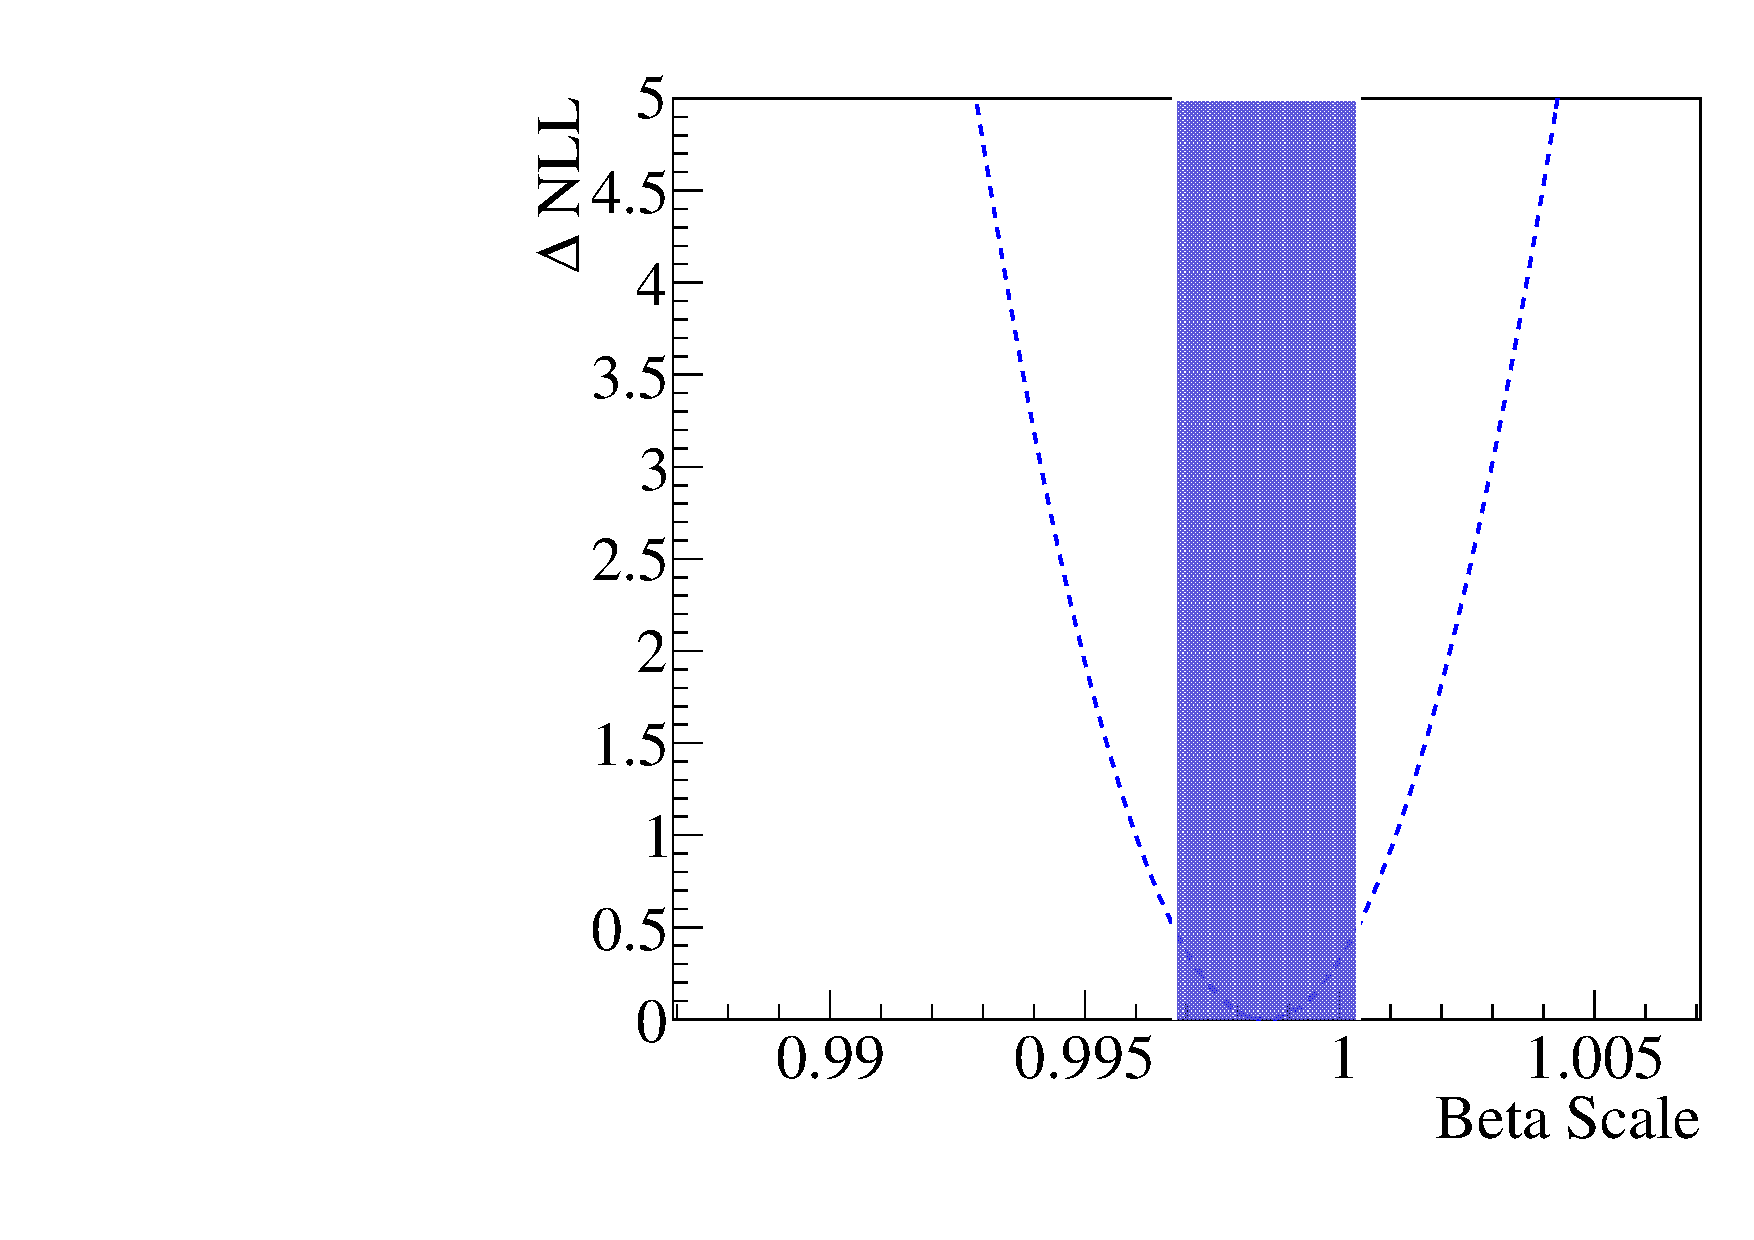
\includegraphics[keepaspectratio=true,height=3in]{NLLProfile_bscale_scan.pdf}
\end{center}
\renewcommand{\baselinestretch}{1}
\small\normalsize
\begin{quote}
\caption{The fit provides constraints on the beta-scale.  Figure provided by Liangjian Wen.}
\label{fig:BetaScaleNLL}
\end{quote}
\end{figure}
\renewcommand{\baselinestretch}{2}
\small\normalsize

Furthermore, it is expected that betas and gammas may need to be calibrated separately.  To a first approximation, gammas deposit energy in the detector by exciting electrons, so these processes should be quite similar.  However, to account for possible differences, we define a beta-scale $\beta$ which quantifies a linear calibration offset between beta and gamma deposits:
\begin{equation}
E_\beta = \beta E_\gamma.
\end{equation}
The beta scale is permitted to float, and is constrained by the fit; figure~\ref{fig:BetaScaleNLL} shows the NLL profile with various choices of beta scale, and demonstrates that it is possible to constrain the beta scale to a value close to $1$ using only the spectral information in the fit.  Uncertainty on the beta scale is incorporated by permitting it to float freely.  We note that currently the beta scale is implemented by shifting beta-like PDF components ($\beta\beta 0\nu$, $\beta\beta 2\nu$, $^{135}$Xe, $^{137}$Xe) relative to the other components which are gamma-like; this ignores the detail that some events may contain clusters generated through both beta and gamma interactions, such as pair production from energetic gammas.  These issues will be addressed in a future analysis, but for now the beta scale is assigned only to decays whose primary particle is a beta~\cite{FittingDocument}.

\begin{figure}
\begin{center}
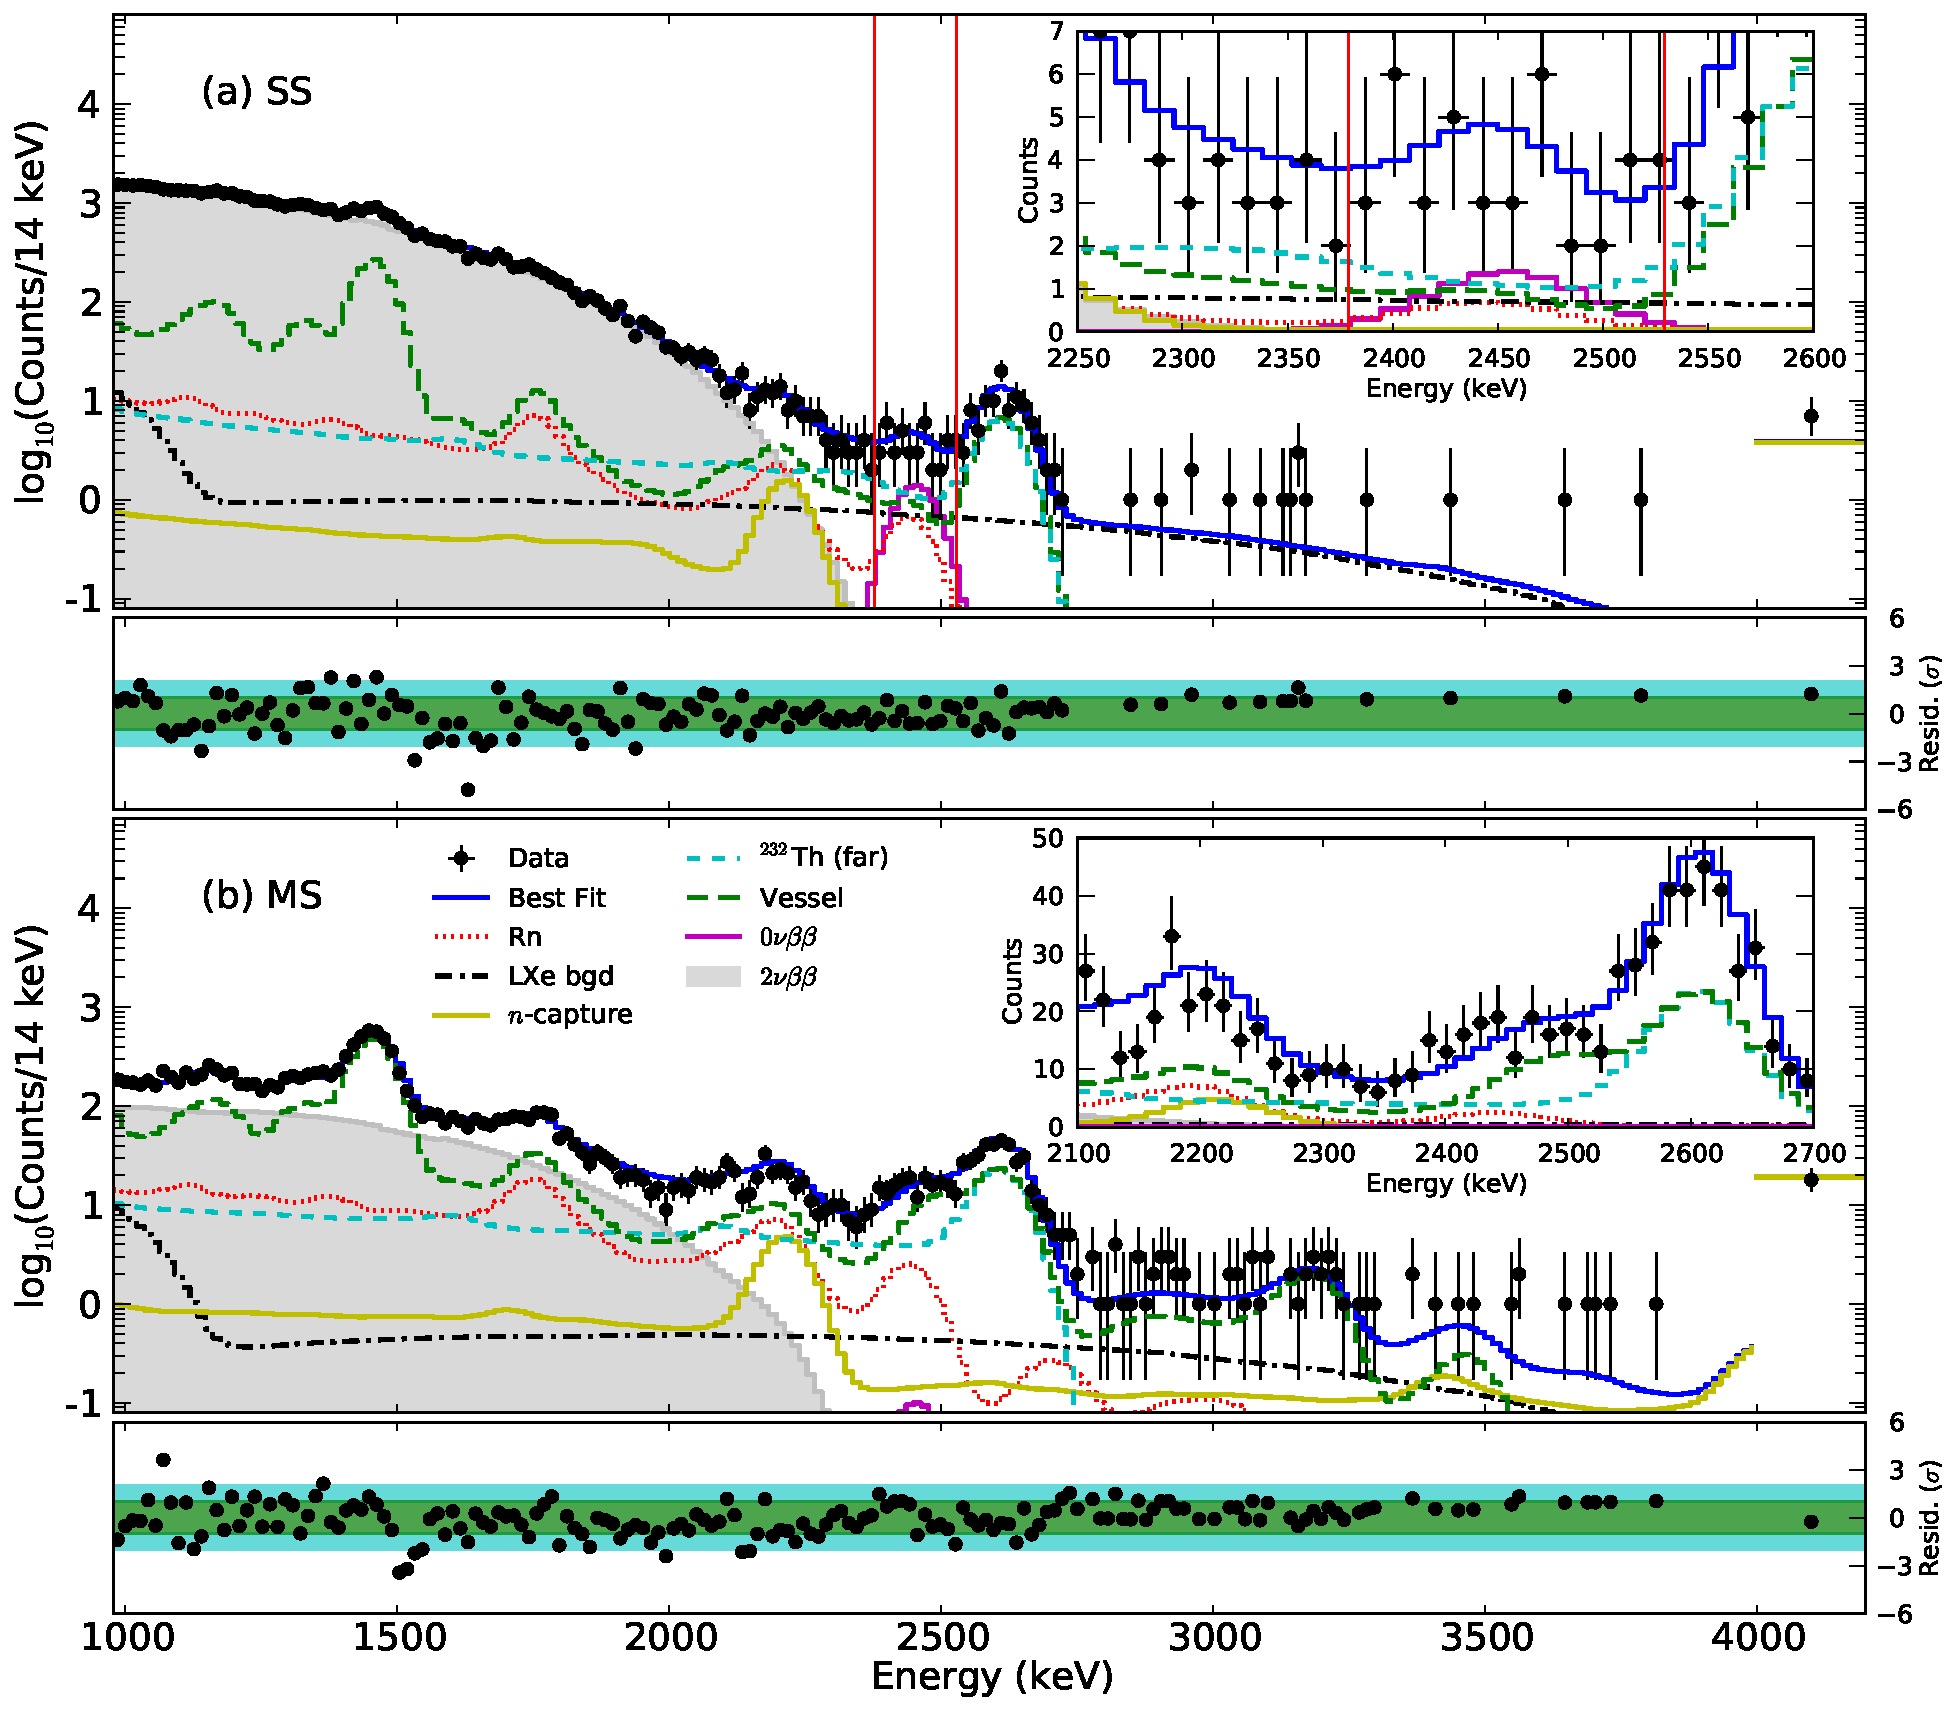
\includegraphics[keepaspectratio=true,width=\textwidth]{Energy_BestFit_frompaper.pdf}
\end{center}
\renewcommand{\baselinestretch}{1}
\small\normalsize
\begin{quote}
\caption{Energy specra with best-fit PDFs for single-site (top) and multi-site (bottom).  Residuals between data and the combined PDFs are shown below the spectra.  The last bin of the spectra is an overflow bin.  The $2\sigma$ region of interest around the $Q$-value is shown on the single-site spectrum.  Insets for single-site and multi-site zoom around the $Q$-value.  The simultaneous standoff-distance fit is not shown~\cite{NewEXObb0nPaper_2014}.}
\label{fig:BestFitEnergyFromPaper}
\end{quote}
\end{figure}
\renewcommand{\baselinestretch}{2}
\small\normalsize

When all of this is done, it is possible to obtain a fit to the low-background spectrum; the maximum-likelihood fit is shown in figure~\ref{fig:BestFitEnergyFromPaper}.  The best-fit expected background in the $2\sigma$ single-site energy window around our $Q$-value is $31.1 \pm 1.8\text{(stat)} \pm 3.3\text{(sys)}$ counts, corresponding to a background rate of $(1.7 \pm 0.2)\cdot 10^{-3} \text{keV}^{-1} \text{kg}^{−1} \text{yr}^{−1}$.  The backgrounds in this $2\sigma$ energy window come from the thorium decay chain ($51\%$), uranium decay chain ($26\%$), and $^{137}$Xe ($23\%$), with other contributions negligible.  The observed event count in the $2\sigma$ single-site energy window is $39$ counts~\cite{NewEXObb0nPaper_2014}.

\begin{figure}
\begin{center}
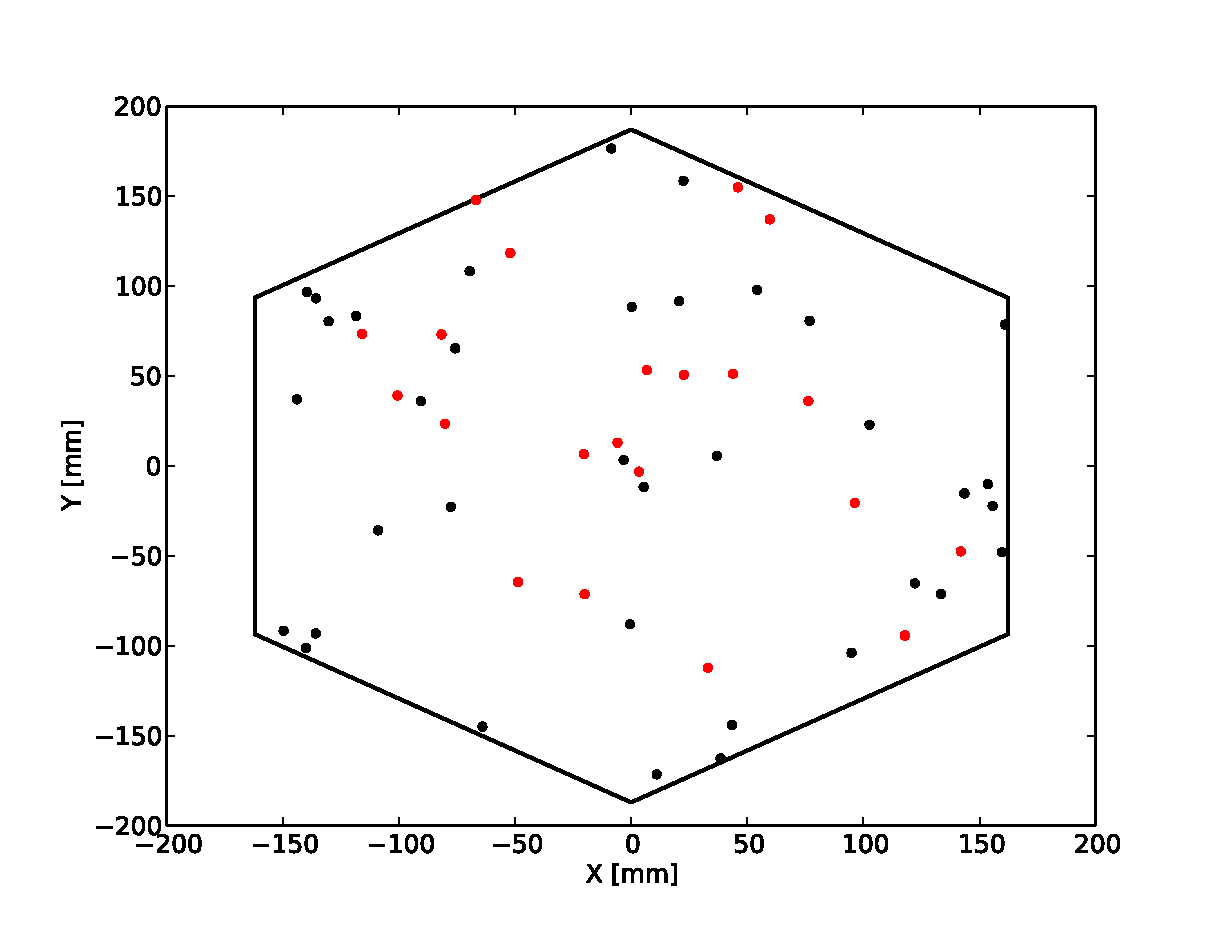
\includegraphics[keepaspectratio=true,width=.49\textwidth]{ROIdistribution_XY.eps}
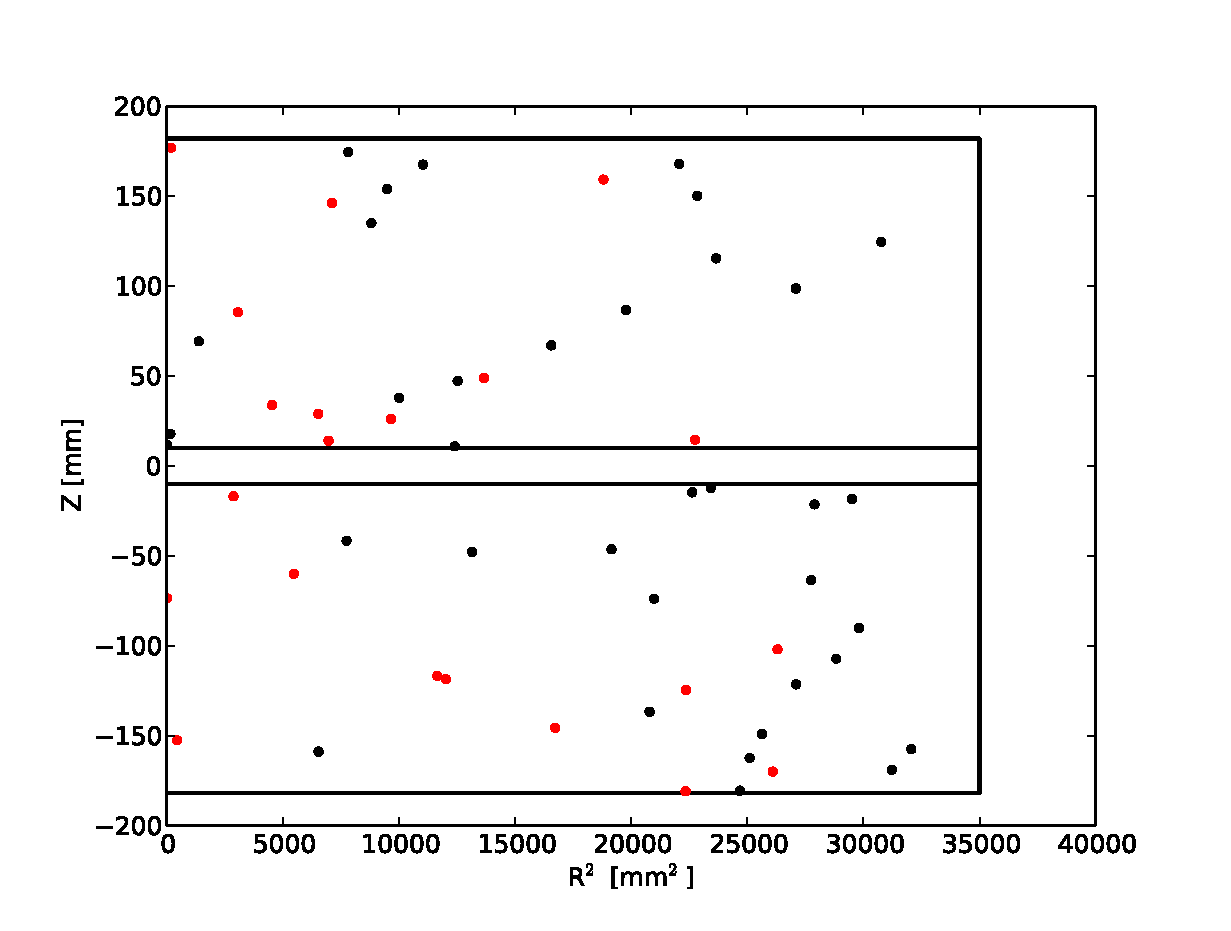
\includegraphics[keepaspectratio=true,width=.49\textwidth]{ROIdistribution_RZ.eps}
\end{center}
\renewcommand{\baselinestretch}{1}
\small\normalsize
\begin{quote}
\caption{The positions of events in the $1\sigma$ region of interest (red) and wider energy range $2325-2550$ keV (black) are shown projected onto their X-Y (left) and $R^2$-Z (right) coordinates.  Lines indicate the fiducial volume, with the dotted lines indicating the fiducial cut away from the cathode that is not used as a component to the standoff distance observable. Figure provided by Dave Moore.}
\label{fig:ROIEventPositionDistribution}
\end{quote}
\end{figure}
\renewcommand{\baselinestretch}{2}
\small\normalsize

(We remind the reader at this point that the quoted limit on $\beta\beta 0\nu$ is not simply based on this comparison of counts, but based on the full set of energy and standoff-distance spectral information.  Representative position information can be seen in figure~\ref{fig:ROIEventPositionDistribution}.  However, the simple comparison of counts can be instructive as an easier-to-understand approximation to the following limits.)

\begin{figure}
\begin{center}
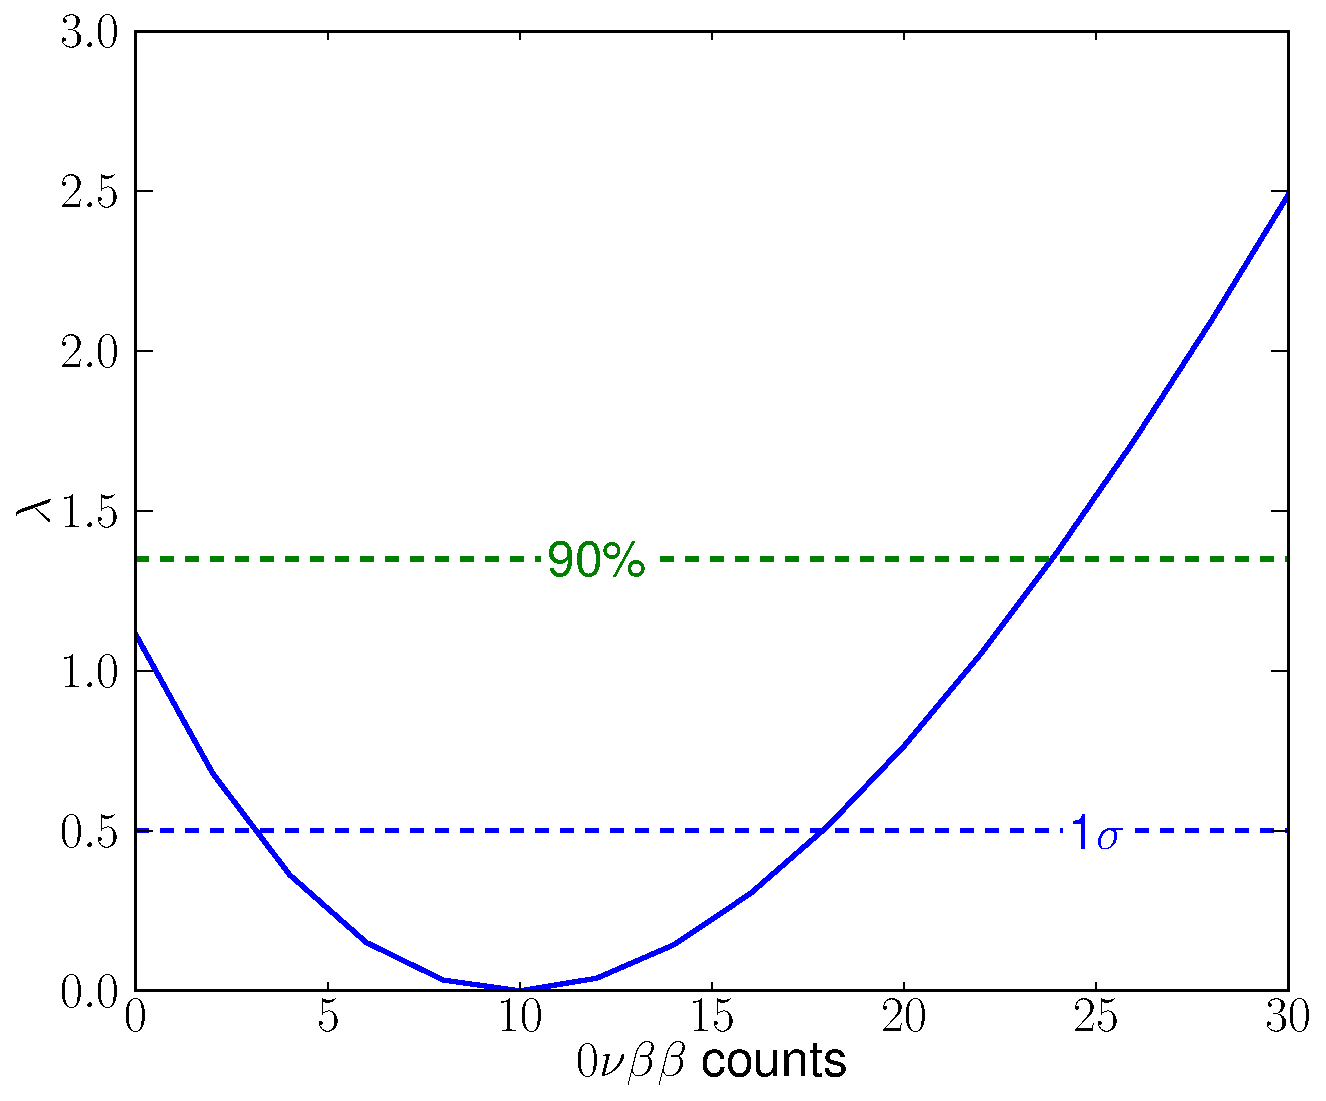
\includegraphics[keepaspectratio=true,height=3in]{0nubb_profile_frompaper.pdf}
\end{center}
\renewcommand{\baselinestretch}{1}
\small\normalsize
\begin{quote}
\caption{Profile scan of negative log-likelihood as a function of the number of fit $\beta\beta 0\nu$ counts~\cite{NewEXObb0nPaper_2014}.}
\label{fig:bb0nProfileFromPaper}
\end{quote}
\end{figure}
\renewcommand{\baselinestretch}{2}
\small\normalsize

The likelihood profile for the total number of $\beta\beta 0\nu$ counts occurring in our detector during the lifetime of the experiment is shown in figure~\ref{fig:bb0nProfileFromPaper}.  Based on the profile, we can see that a $1\sigma$ confidence interval for this parameter would exclude the null hypothesis of zero $\beta\beta 0\nu$ counts; however, only $1\sigma$ exclusion of the null hypothesis is far too weak to make an inference of a non-zero signal.  Instead, we follow the conventions of the field and quote a $90\%$-confidence upper limit of $24$ total counts from $\beta\beta 0\nu$.  This corresponds to a $90\%$-confidence lower limit on the halflife of $^{136}$Xe decay by the $\beta\beta 0\nu$ mode of $1.1 \cdot 10^{25}$ years~\cite{NewEXObb0nPaper_2014}.

\section{Results and Physics Reach}\label{sec:ResultResults}

We have stated the half-life limit on $\beta\beta 0\nu$ decay of $^{136}$Xe, which is the main result of the present analysis.  We shall now continue to put this result in context with the expected sensitivity of the experiment and compare it to the limits and sensitivities achieved by other leading $\beta\beta 0\nu$ experiments.

To place the limit derived with the current dataset in context with the overall strength of the experiment, we generate a number of toy Monte Carlo datasets.  We assume that our best-fit backgrounds are fully accurate and that the null hypothesis (no $\beta\beta 0\nu$) is true; we then use this best-fit background as our PDF and generate toy datasets.  These can be used to study the ``typical'' results our detector would have produced if the same experiment could be repeated many times.

\begin{figure}
\begin{center}
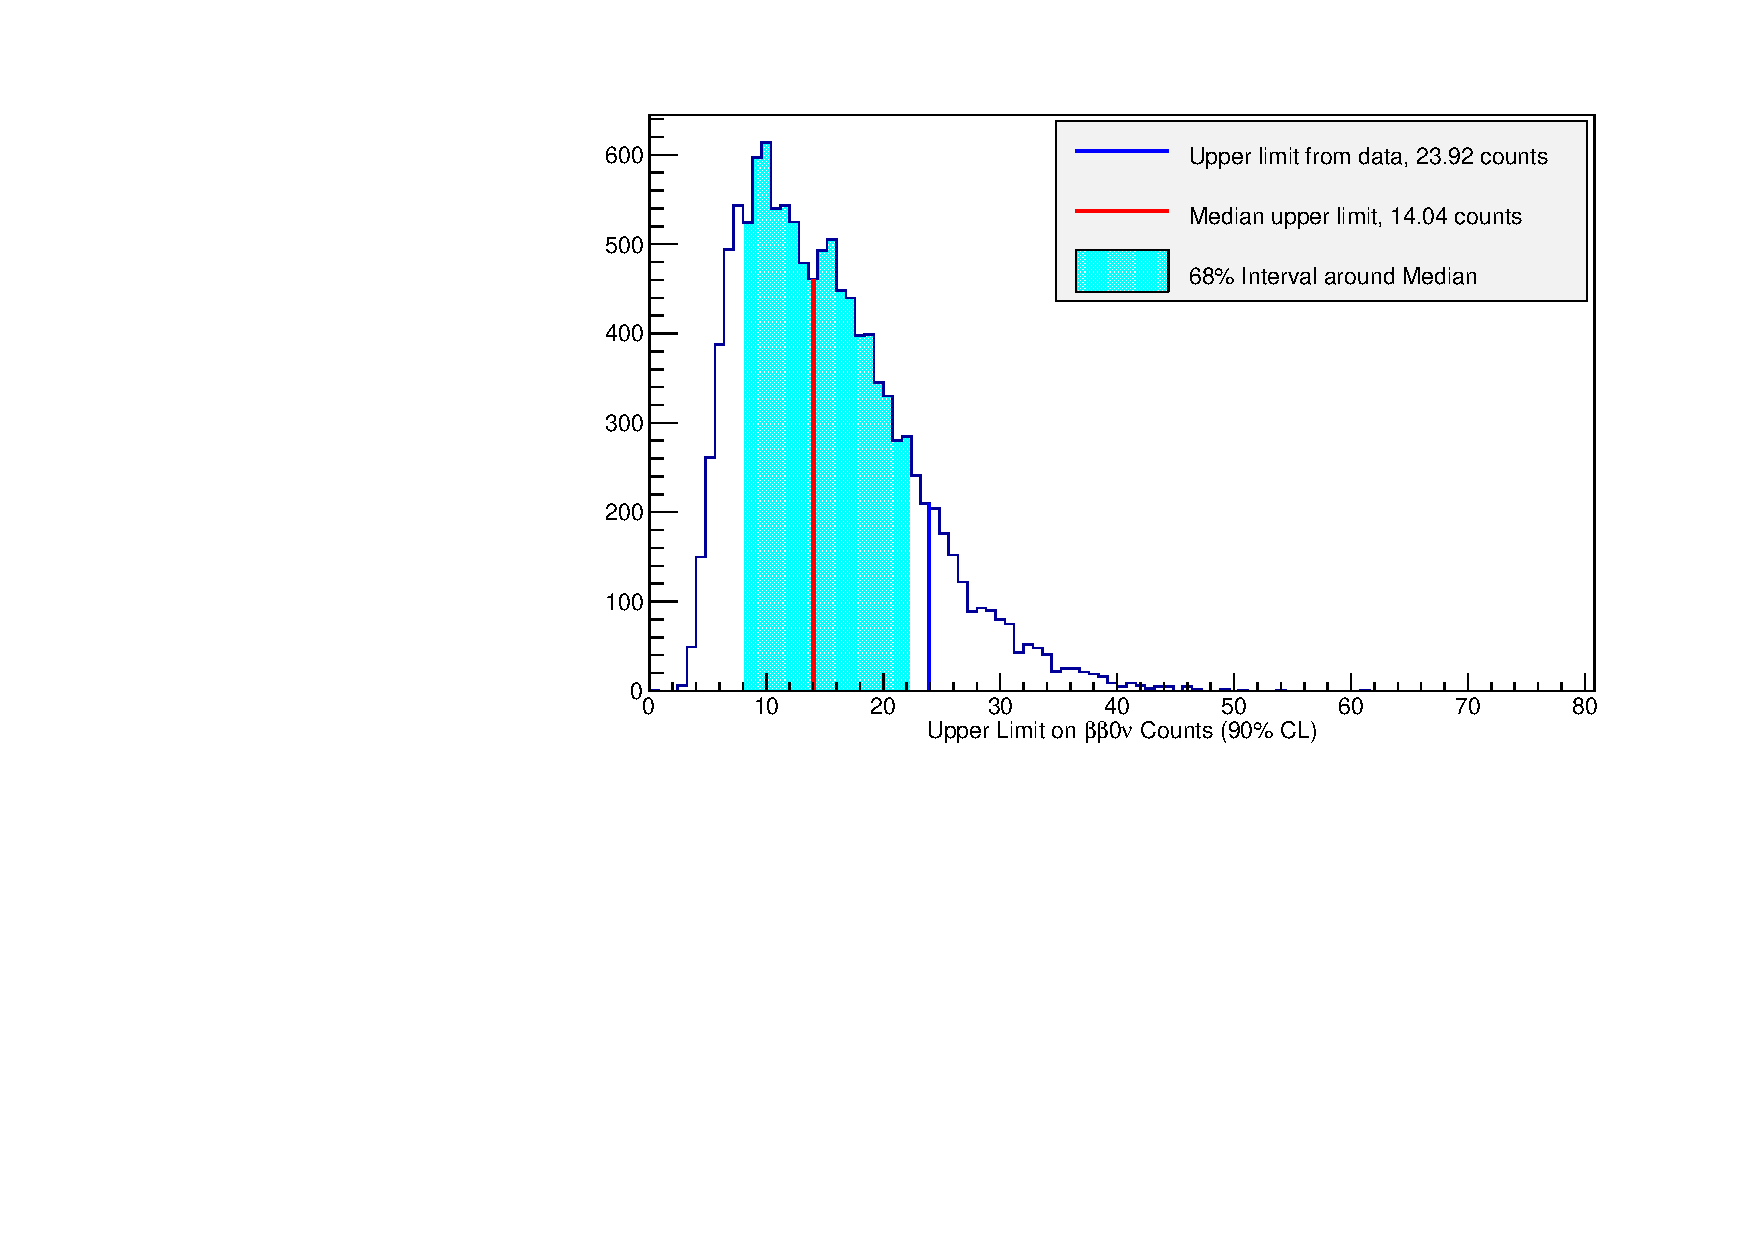
\includegraphics[keepaspectratio=true,width=.9\textwidth]{toy_mc_sensitivity.pdf}
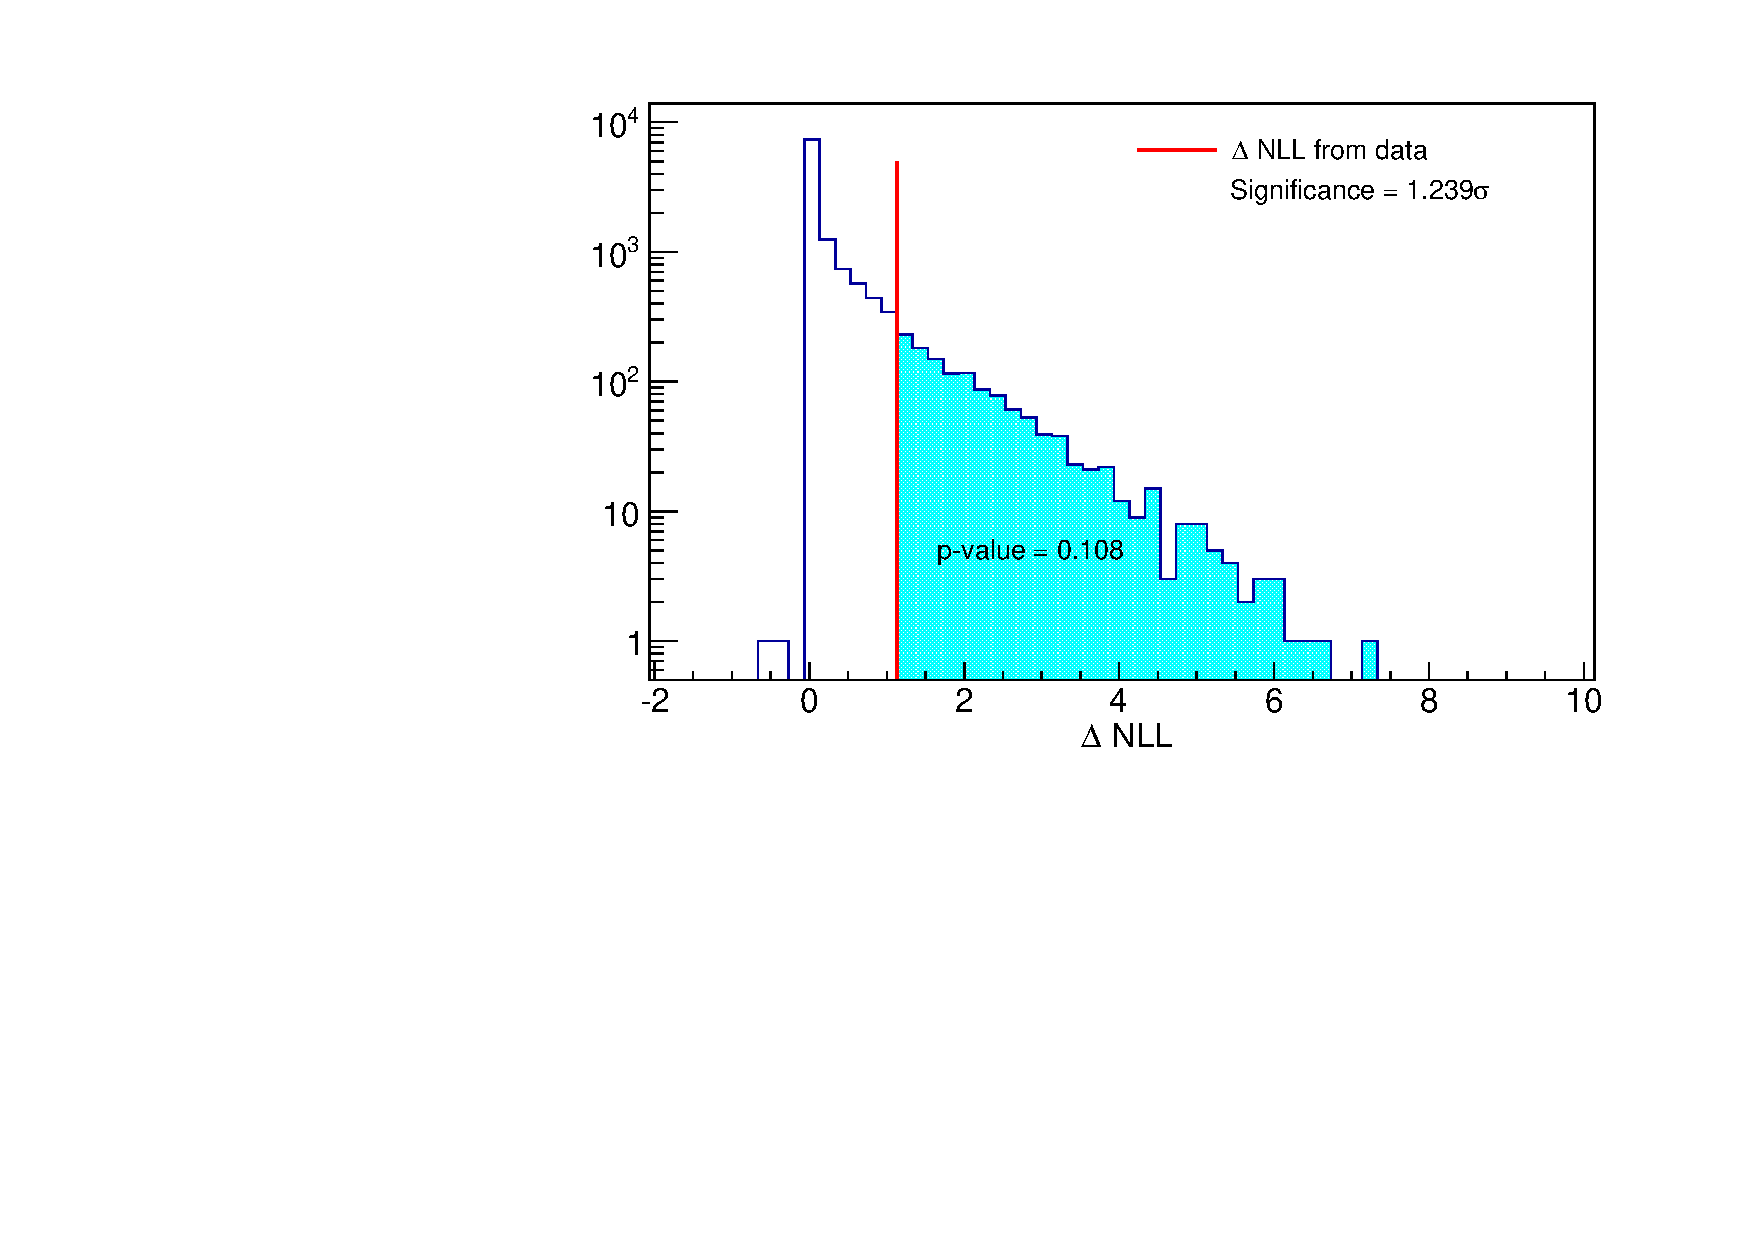
\includegraphics[keepaspectratio=true,width=.9\textwidth]{toy_mc_significance.pdf}
\end{center}
\renewcommand{\baselinestretch}{1}
\small\normalsize
\begin{quote}
\caption{Assuming that the background measurements of EXO-200 from this analysis are accurate, toy datasets are simulated.  The top plot shows the probability distribution of our $90\%$ confidence limit; we find that our median upper limit is 14.04 counts attributed to $\beta\beta 0\nu$, compared to our observed upper limit of 23.92 counts.  The bottom plot shows the probability distribution of our ability to reject the null hypothesis (no $\beta\beta 0\nu$) based on the negative log-likelihood; we find that the present dataset rejects the null hypothesis with probability less than $90\%$.  Figures provided by Ryan Killick.}
\label{fig:ToyMCSensitivitySelectivity}
\end{quote}
\end{figure}
\renewcommand{\baselinestretch}{2}
\small\normalsize

The resulting distributions are shown in figure~\ref{fig:ToyMCSensitivitySelectivity}.  The top plot shows the distribution of $90\%$-confidence upper limits on the number of $\beta\beta 0\nu$ counts; we can see that typical datasets from the EXO-200 experiment result in limits ranging from 8 to 22 counts.  The median limit, is 14 counts; this value is called the median sensitivity, and it illustrates the overall strength of an experiment.  We contrast this with the observed limit of 24 counts; as is apparent from the distribution, this limit is consistent with an unlucky upward fluctuation in the backgrounds observed by EXO-200.

We saw in the NLL profile on the total number of $\beta\beta 0\nu$ counts in figure~\ref{fig:bb0nProfileFromPaper} that the NLL for the hypothesis of no $\beta\beta 0\nu$ counts is about 1.1 higher than for the best fit; this quantity reflects how well we can reject the null hypothesis in favor of the best fit.  To put this in context, we also observe the distribution of this value from toy Monte Carlo datasets in the bottom plot of figure~\ref{fig:ToyMCSensitivitySelectivity}.  Here, we see that $10.8\%$ of identical experiments will yield an NLL profile which is at least 1.1 worse for no $\beta\beta 0\nu$ than for the best fits even though no $\beta\beta 0\nu$ is simulated.  We can conclude that this difference in NLL is not strong enough to reject the null hypothesis with high confidence.

\begin{figure}
\begin{center}
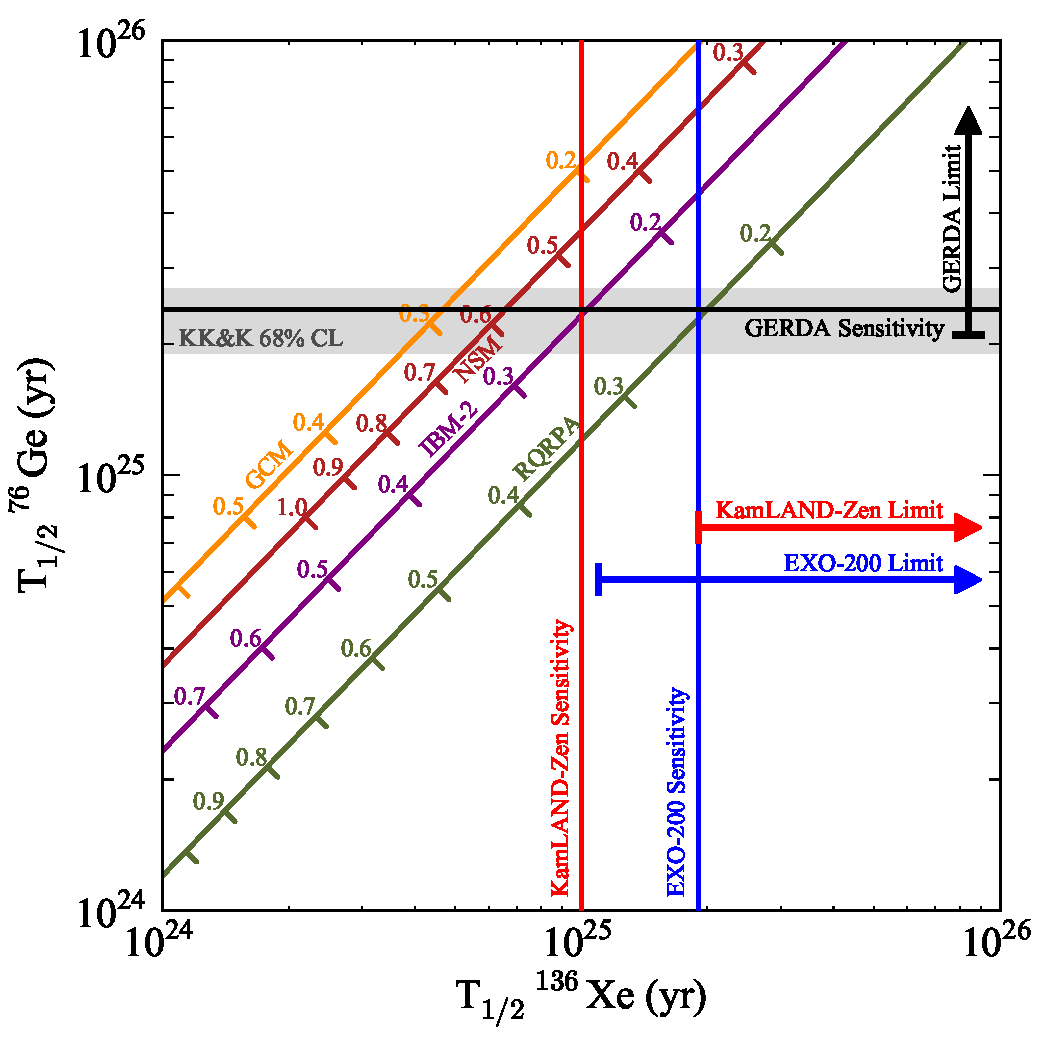
\includegraphics[keepaspectratio=true,width=\textwidth]{MatplotLibSensitivity.pdf}
\end{center}
\renewcommand{\baselinestretch}{1}
\small\normalsize
\begin{quote}
\caption{$\beta\beta 0\nu$ constraints are shown from $^{136}$Xe (horizontal) and $^{76}$Ge (vertical).  The four diagonal lines represent four recent matrix element computations \cite{PhysRevLett.105.252503,Menéndez2009139,PhysRevC.87.014315,PhysRevC.87.045501} and one recent phase-space factor~\cite{PhysRevC.85.034316} relating the two half-lives; tick marks along the diagonal represent the corresponding mass $\left<m_{\beta\beta}\right>$.  $90\%$ confidence limits and median $90\%$ sensitivities are shown for the KamLand-Zen~\cite{PhysRevLett.110.062502}, GERDA~\cite{PhysRevLett.111.122503}, and EXO-200 experiments~\cite{NewEXObb0nPaper_2014}; the claimed 2006 discovery by Klapdor-Kleingrothaus and Krivosheina is shown as a $1\sigma$ confidence interval~\cite{Klapdor}.}
\label{fig:MatplotlibSensitivity}
\end{quote}
\end{figure}
\renewcommand{\baselinestretch}{2}
\small\normalsize

The wide spread of limits produced in toy Monte Carlo studies illustrates the significant role that luck plays in the limits set by low-statistics experiments such as EXO-200.  To compare EXO-200 to other experiments, it is useful to compare both the limits and the median sensitivities (median $90\%$ confidence limits).  This is done in figure~\ref{fig:MatplotlibSensitivity}.  Vertical lines correspond to the reported median sensitivities of the two leading $^{136}$Xe experiments, KamLAND-Zen and EXO-200; right-pointing arrows indicate the actual limits set by each.  For both experiments we can see that statistical fluctuations in the background account for factor-of-two differences between median sensitivity and observed limits; EXO-200 claims to be the most sensitive $^{136}$Xe experiment, but KamLAND-Zen currently reports the strongest limit.  Both experiments intend to continue running, and EXO-200 hopes that their next dataset is atypical in the other way.

Nuclear matrix elements have large uncertainties, as described in \ref{sec:NuclearMatrixCalculations}.  Figure~\ref{fig:MatplotlibSensitivity} illustrates four diagonal lines corresponding to four different modern nuclear matrix calculations, and uses these values to relate the half-lives of $^{136}$Xe and $^{76}$Ge.  The current median sensitivity and limit on the $\beta\beta 0\nu$ half-life of $^{76}$Ge from GERDA are shown as a horizontal line and vertical arrow, respectively.  This is contrasted with the 2006 claimed discovery by Klapdor-Kleingrothaus and Krivosheina of $\beta\beta 0\nu$ decay, which is not excluded by the more recent GERDA limit.

Furthermore, the nuclear matrix elements permit us to translate half-life lower limits into upper limits on the effective Majorana neutrino mass $\left<m_{\beta\beta}\right>$.  The relation is indicated, for each choice of nuclear matrix elements, by tick marks on the corresponding diagonal line.  We can see that the GERDA and EXO-200 experiments are of similar strengths, depending most on the choice nuclear matrix elements; KamLAND-Zen is comparable in strength to GERDA for the RQRPA nuclear matrix elements, and stronger for all other choices in this plot.  The $90\%$-confidence mass limit quoted by EXO-200 is $\left<m_{\beta\beta}\right> < 190-450$ meV, depending on the choice of matrix elements.  Recalling figure~\ref{fig:NeutrinoMassBounds}, this corresponds to a $90\%$-confidence limit on the mass of the lightest neutrino eigenstate of $m_{min} < 0.69–1.63$ eV under the most conservative choice of Majorana phases~\cite{NewEXObb0nPaper_2014}.

\section{Comparison to Results without Denoising}\label{sec:ResultComparison}

The results presented in section~\ref{sec:ResultResults} are obtained using the most up-to-date analysis techniques adopted by the EXO-200 collaboration.  These include the denoising technique described in chapter~\ref{ch:DenoisingTheory}.  In this section we compare physics results with and without denoising and demonstrate the degree to which resolution gains from denoising strengthen the EXO-200 result.  We begin with a comparison of the energy measurements in section~\ref{sec:ResultComparisonEnergy}, and then proceed to a comparison of the physics results in section~\ref{sec:ResultComparisonPhysics}.

\subsection{Comparison of Energy Resolution and Calibration}\label{sec:ResultComparisonEnergy}

\begin{table}
\begin{center}
\begin{tabular}{|c|c|c|c|c|}
\hline \multirow{2}{*}{Parameter} & \multicolumn{2}{|c|}{Undenoised} & \multicolumn{2}{|c|}{Denoised}\\
\cline{2-5}& SS & MS & SS & MS \\
\hline $p_0$ & 0 & 0 & 0.628 & 0.602 \\
\hline $p_1$ & 39.8 & 43.0 & 20.8 & 25.8 \\
\hline $p_2$ & 0.0107 & 0.0096 & 0.0011 & 0.0040 \\
\hline \% $\sigma/E$ at $Q$-value & 1.94 & 2.00 & 1.53 & 1.65 \\ \hline
\end{tabular}
\end{center}
\caption{Time-averaged resolution parameters for denoised and undenoised data.  For undenoised data, measurements were consistent with $p_0 = 0$, so this parameter was not used in the analysis of undenoised data.  The resulting time-averaged resolutions at our $Q$-value are also shown~\cite{AverageEnergyResolutionDocument}.}
\label{tab:ResolutionFunctions_DenoisedUndenoisedComparison}
\end{table}

\begin{figure}
\begin{center}
\includegraphics[keepaspectratio=true,width=.95\textwidth]{ResolutionFunctionComparison_absolute.pdf}
\includegraphics[keepaspectratio=true,width=.95\textwidth]{ResolutionFunctionComparison_relative.pdf}
\end{center}
\renewcommand{\baselinestretch}{1}
\small\normalsize
\begin{quote}
\caption{The time-averaged resolution functions (top) and relative resolution functions (bottom) are compared for denoised and undenoised data.  Bands indicate uncertainties.  Data provided by Caio Licciardi.}
\label{fig:ResolutionFunctionComparison}
\end{quote}
\end{figure}
\renewcommand{\baselinestretch}{2}
\small\normalsize

The energy resolution parameters with and without denoising, using the parametrization defined in equation~\ref{eqn:ResolutionAbsoluteFunctionForm}, are listed in table~\ref{tab:ResolutionFunctions_DenoisedUndenoisedComparison}.  The undenoised resolution functions have fixed $p_0 = 0$ because fits with undenoised data led to resolution functions consistent with zero.  The resolution functions are compared in figure~\ref{fig:ResolutionFunctionComparison}.  The resolution at our $Q$-value is also indicated in table~\ref{tab:ResolutionFunctions_DenoisedUndenoisedComparison}; in single-site data we can see that implementing denoising improves our energy resolution at the $Q$-value from 1.94\% to 1.53\%.

Recalling the interpretation of the resolution parameters which was described in section~\ref{sec:RotatedEnergyResMeasurement} leads to a number of suggestive observations.  First, $p_1$ has decreased by a factor of 1.9 in single-site data and 1.7 in multi-site data when we move from undenoised to denoised resolutions.  The parameter $p_1$ is associated with electronic noise, so we can interpret this to mean that we have indeed reduced the impact of electronic noise after denoising.

Secondly, $p_2$ has decreased by a factor of 2.4 in the multi-site data and a factor of 9.7 for single-site data.  The parameter $p_2$ is associated with improper gain calibrations; the old method of APD reconstruction handled only a simple sum of APD waveforms with no APD channel gain corrections, whereas the lightmap used with denoising has detailed time-dependent gain information for every channel built into it.  Thus, the reduction in $p_2$ may be a reflection of the impact of improved APD gain information on our energy resolution.

And finally, $p_0$ is observed to increase from a value consistent with zero to the dominant component of the denoised resolution at our $Q$-value.  The parameter $p_0$ is associated with Poisson fluctuations in the number of photons detected.  In the old method of APD reconstruction we always used a sum of all APD waveforms for scintillation measurements; implicitly, we were always using the full light collecting efficiency of the EXO-200 detector.  By contrast, denoising is designed with the flexibility to weight fewer APD channels more heavily, effectively sacrificing light collection for the benefit of a reduction in electronic noise.  It is likely that $p_0$ is zero with undenoised data because Poisson fluctuations in the total light collection of EXO-200 are small, whereas denoising uses a sufficiently small number of APD channels that Poisson fluctuations become important.  Moreover, we recall in section~\ref{sec:DenoisingInPractice} that the current analysis mistakenly underestimates Poissonian noise produced inside the APDs, and this would manifest itself by subjecting the scintillation estimate to even more statistical fluctuations than would be ideal.  We can imagine that when this error is corrected in future analyses the $p_0$ parameter may respond by decreasing, possibly at the expense of a larger $p_0$ value as more channels are used.

It should be noted that although these interpretations of $p_0$, $p_1$, and $p_2$ are highly suggestive, they depend on the assumption that scintillation energy resolution continues to be the dominant factor in our rotated energy resolution at all energy scales.  As an alternative, it has been suggested that the rotation angle may have an energy dependence which is not described by our calibrations~\cite{EnergyDocumentRun2a}; failure to include this dependence may be reflected by an energy dependence in the resolution function which does not agree with the interpretation we provide here.  Also, the error bands in figure~\ref{fig:ResolutionFunctionComparison} are still somewhat broad, and more accurate resolution measurements from a wider range of energies would be useful to constrain the values of these parameters better.  Further investigation will be required to verify that the scintillation energy measurement accuracy is still the dominant contributor to energy resolution at all energy scales.

\begin{figure}
\begin{center}
\includegraphics[keepaspectratio=true,width=\textwidth]{RotatedReso_denoised_compVsTime.pdf}
\end{center}
\renewcommand{\baselinestretch}{1}
\small\normalsize
\begin{quote}
\caption{Time dependence of the single-site energy resolution at $2615$ keV with denoised (blue) and undenoised (red) scintillation.  Time-averaged energy resolutions at this energy (1.47\% denoised, 1.86\% undenoised) are overlaid as dashed lines.  Data provided by Mike Marino.}
\label{fig:ResolutionTimeDependenceComparison}
\end{quote}
\end{figure}
\renewcommand{\baselinestretch}{2}
\small\normalsize

We also find that the time-dependence of the energy resolution has been dramatically affected by denoising.  Figure~\ref{fig:ResolutionTimeDependenceComparison} compares the single-site energy resolutions at the $^{208}$Tl 2615 keV gamma line with denoised and undenoised data, as measured from $^{232}$Th source calibration data.  The denoised energy resolution varies by as much as 0.3 percentage points, but the undenoised energy resolution varies by as much as 0.6 percentage points.  We saw in figure~\ref{fig:ResolutionAPDNoiseComparison} that the energy resolution of the detector was strongly correlated with APD noise, but after denoising this effect is significantly reduced.  In particular, the period of particularly poor energy resolution November 2012 and May 2013 is no longer exceptional, indicating that this poor energy resolution came from noise which denoising can reduce to negligible levels~\cite{NewEXObb0nPaper_2014}.

\begin{figure}
\begin{center}
\includegraphics[keepaspectratio=true,width=.49\textwidth]{nonLinearity_ss.pdf}
\includegraphics[keepaspectratio=true,width=.49\textwidth]{nonLinearity_ms.pdf}
\end{center}
\renewcommand{\baselinestretch}{1}
\small\normalsize
\begin{quote}
\caption{The non-linearity of the calibration is shown here for denoised (red) and undenoised (black) data in single-site (left) and multi-site (right).  $R_{rec}$ is defined as the ratio between the observed peak position and the observed peak position of the $2615$ keV $^{232}$Th peak, and $R_{real}$ is defined as the true ratio between the peak position and 2615 keV; the vertical axis shows the relative difference between $R_{rec}$ and $R_{real}$, which reflects how much non-linear correction the calibration must perform.  The cesium, cobalt, and thorium peaks (662, 1173, 1332, and 2615 keV) are used to obtain a calibration; the radium line at 2448 keV and the neutron capture line from hydrogen at 2200 keV are shown as cross-checks~\cite{EnergyDocumentRun2ab}.}
\label{fig:NonLinearityOfCalibrationComparison}
\end{quote}
\end{figure}
\renewcommand{\baselinestretch}{2}
\small\normalsize

One concern with the denoised energy calibration comes from the observed non-linearity of the observation, shown in figure~\ref{fig:NonLinearityOfCalibrationComparison}.  The ratio of reconstructed peak positions become farther from what we expect with denoised energy, indicating more significant contributions from the $E_{bias}$, $p_0$, and $p_2$ parameters of the calibration defined in equation~\ref{eqn:EnergyCalibrationParametrization}.  This is not in itself a problem -- it is the job of calibration to correct for such things -- but as the calibration changes more rapidly with energy it becomes important for us to constrain it with more calibration points at a wide range of energies.  Starting in June 2013 we have a $^{226}$Ra source which contains many gamma lines, including its primary line at 2448 keV which serves as an excellent constraint for the energy of our $Q$-value.  For existing data, there is some hope of using the lower-energy gamma lines of the $^{228}$Th source, visible in figure~\ref{fig:LiangjianRotatedSpectrumImprovement}, as a new set of calibration points which is accessible due to the improved resolution of the denoised dataset.

\subsection{Comparison of Physics Results}\label{sec:ResultComparisonPhysics}

We now proceed to compare the physics results obtained with denoising to those which would have been obtained without denoising.  We recall from figure~\ref{fig:BackgroundVsResolution} that improvement of the energy resolution will have the strongest effect on our $^{232}$Th backgrounds, and will have a smaller (but not negligible) effect on our $^{137}$Xe backgrounds.  Here we will show changes as they impact our $2\sigma$ region of interest, and will conclude with a comparison of the profile likelihood scans obtained from full fits to the spectrum.

We begin by listing the events which occur in the denoised single-site spectrum in the energy window from 2325 to 2550 keV.  These are provided in table~\ref{tab:EventTable_DenoisedWideRegion}, which also includes the corresponding undenoised energy and the change in energy due to denoising.  The table indicates whether the event would fall within the $2\sigma$ region of interest in both the denoised and undenoised analysis.

\begin{center}
\begin{longtable}{|c|c|c|c|c|c|c|}
\caption{All single-site events which fall into the denoised energy window between 2325 and 2550 keV.  This fully includes the $2\sigma$ window around the $Q$-value; we indicate whether the event falls into that $2\sigma$ window.  The correponding undenoised energy  is also indicated, along with whether that undenoised energy falls into the undenoised $2\sigma$ region of interest.}\label{tab:EventTable_DenoisedWideRegion}\\

\hline \multirow{2}{*}{Run\#} & \multirow{2}{*}{Event\#} & \multicolumn{2}{|c|}{Denoised} & \multicolumn{2}{|c|}{Undenoised} & \multirow{2}{*}{$\Delta$E (keV)} \\
\cline{3-6} & & Energy (keV) & In ROI? & Energy (keV) & In ROI? &  \\ \hline
\endfirsthead

\multicolumn{7}{c}
{{\bfseries \tablename\ \thetable{} -- continued from previous page}} \\
\hline \multirow{2}{*}{Run\#} & \multirow{2}{*}{Event\#} & \multicolumn{2}{|c|}{Denoised} & \multicolumn{2}{|c|}{Undenoised} & \multirow{2}{*}{$\Delta$E (keV)} \\
\cline{3-6} & & Energy (keV) & In ROI? & Energy (keV) & In ROI? &  \\ \hline
\endhead

\hline \multicolumn{7}{|r|}{{Continued on next page}} \\ \hline
\endfoot

\hline
\endlastfoot

\hline 2669 & 3889 & 2327.4 & No & 2322.6 & No & 4.8 \\
\hline 2782 & 2237 & 2464.2 & Yes & 2560.3 & No & -96.0 \\
\hline 2831 & 4864 & 2488.5 & Yes & 2245.3 & No & 243.2 \\
\hline 3155 & 2053 & 2524.6 & Yes & 2541.6 & Yes & -17.0 \\
\hline 3155 & 6861 & 2448.5 & Yes & 2403.4 & Yes & 45.1 \\
\hline 3255 & 8687 & 2360.4 & No & 2353.4 & No & 7.0 \\
\hline 3321 & 8688 & 2332.4 & No & 2315.2 & No & 17.2 \\
\hline 3461 & 845 & 2357.7 & No & 2336.6 & No & 21.1 \\
\hline 3573 & 1958 & 2406.1 & Yes & 2421.4 & Yes & -15.2 \\
\hline 3657 & 3515 & 2417.0 & Yes & 2399.1 & Yes & 17.8 \\
\hline 3740 & 11325 & 2405.7 & Yes & 2324.8 & No & 80.9 \\
\hline 3912 & 10712 & 2391.3 & Yes & 2399.8 & Yes & -8.5 \\
\hline 3933 & 3459 & 2441.4 & Yes & 2507.3 & Yes & -65.9 \\
\hline 3964 & 9703 & 2459.2 & Yes & 2464.8 & Yes & -5.6 \\
\hline 3972 & 754 & 2509.6 & Yes & 2470.9 & Yes & 38.8 \\
\hline 3994 & 12296 & 2412.7 & Yes & 2367.1 & Yes & 45.5 \\
\hline 4030 & 5037 & 2502.1 & Yes & 2482.8 & Yes & 19.3 \\
\hline 4032 & 2727 & 2426.4 & Yes & 2349.3 & No & 77.1 \\
\hline 4065 & 2350 & 2428.8 & Yes & 2442.8 & Yes & -14.0 \\
\hline 4068 & 8841 & 2543.4 & No & 2640.4 & No & -97.0 \\
\hline 4068 & 9897 & 2423.9 & Yes & 2453.5 & Yes & -29.7 \\
\hline 4078 & 2595 & 2370.3 & No & 2372.4 & Yes & -2.0 \\
\hline 4229 & 9176 & 2541.3 & No & 2519.5 & Yes & 21.9 \\
\hline 4258 & 13386 & 2340.7 & No & 2338.8 & No & 2.0 \\
\hline 4288 & 1334 & 2333.9 & No & 2340.6 & No & -6.7 \\
\hline 4288 & 11179 & 2466.0 & Yes & 2494.1 & Yes & -28.1 \\
\hline 4288 & 13040 & 2418.6 & Yes & 2486.3 & Yes & -67.7 \\
\hline 4306 & 10543 & 2544.3 & No & 2574.1 & No & -29.7 \\
\hline 4373 & 3036 & 2349.4 & No & 2395.3 & Yes & -45.8 \\
\hline 4378 & 11150 & 2492.3 & Yes & 2494.2 & Yes & -1.9 \\
\hline 4402 & 10759 & 2393.0 & Yes & 2398.0 & Yes & -5.1 \\
\hline 4433 & 16390 & 2529.9 & No & 2494.1 & Yes & 35.8 \\
\hline 4459 & 29435 & 2529.3 & No & 2472.2 & Yes & 57.1 \\
\hline 4475 & 11191 & 2454.5 & Yes & 2521.3 & Yes & -66.8 \\
\hline 4490 & 4613 & 2441.5 & Yes & 2481.4 & Yes & -40.0 \\
\hline 4507 & 6129 & 2435.6 & Yes & 2412.4 & Yes & 23.2 \\
\hline 4672 & 1891 & 2383.5 & Yes & 2418.5 & Yes & -35.0 \\
\hline 4705 & 5799 & 2404.6 & Yes & 2465.7 & Yes & -61.1 \\
\hline 4712 & 5996 & 2466.0 & Yes & 2439.5 & Yes & 26.5 \\
\hline 4733 & 3595 & 2364.9 & No & 2381.2 & Yes & -16.2 \\
\hline 4809 & 3937 & 2427.7 & Yes & 2429.1 & Yes & -1.4 \\
\hline 4860 & 5170 & 2513.8 & Yes & 2596.3 & No & -82.5 \\
\hline 4882 & 310 & 2474.2 & Yes & 2450.2 & Yes & 24.1 \\
\hline 4899 & 9833 & 2342.4 & No & 2323.7 & No & 18.7 \\
\hline 4903 & 7366 & 2472.6 & Yes & 2456.7 & Yes & 15.9 \\
\hline 4918 & 4313 & 2377.1 & No & 2458.2 & Yes & -81.1 \\
\hline 4957 & 8387 & 2398.6 & Yes & 2384.9 & Yes & 13.7 \\
\hline 4978 & 6796 & 2521.1 & Yes & 2518.8 & Yes & 2.3 \\
\hline 5010 & 2201 & 2365.3 & No & 2349.5 & No & 15.7 \\
\hline 5082 & 9766 & 2517.7 & Yes & 2477.1 & Yes & 40.6 \\
\hline 5097 & 7670 & 2472.1 & Yes & 2441.0 & Yes & 31.1 \\
\hline 5105 & 15012 & 2548.5 & No & 2559.8 & No & -11.3 \\
\hline 5124 & 7626 & 2480.4 & Yes & 2411.8 & Yes & 68.6 \\
\hline 5305 & 3256 & 2406.0 & Yes & 2393.2 & Yes & 12.8 \\
\hline 5372 & 11466 & 2513.7 & Yes & 2557.9 & No & -44.2 \\
\hline 5380 & 4415 & 2458.2 & Yes & 2478.9 & Yes & -20.7 \\
\hline 5409 & 38 & 2405.1 & Yes & 2456.9 & Yes & -51.8 \\
\end{longtable}
\end{center}

\begin{figure}
\begin{center}
\includegraphics[keepaspectratio=true,width=\textwidth]{DenoisedVsUndenoised_bb0nProfiles.pdf}
\end{center}
\renewcommand{\baselinestretch}{1}
\small\normalsize
\begin{quote}
\caption{Denoised (red) and undenoised (blue) profile likelihood curves for $\beta\beta 0\nu$.}
\label{fig:DenoisedComparison_Profiles}
\end{quote}
\end{figure}
\renewcommand{\baselinestretch}{2}
\small\normalsize

To compare the limits set with denoised and undenoised data, figure~\ref{fig:DenoisedComparison_Profiles} includes the profile likelihood curves derived from both datasets.  The beta scale is included as a systematic here, broadening both curves.  The 90\% confidence limit is the value of $\beta\beta 0\nu$ at which the curve has a value of 1.35; for the denoised data we can set a 90\% confidence limit of 24 counts, whereas with the undenoised data we set a 90\% confidence limit of 27 counts.  This means denoising has given us an 11\% stronger halflife limit than the undenoised dataset could have provided; or, since the neutrino mass $\left<m_{\beta\beta}\right>$ is proportional to the square root of halflife, denoising gives us a 6\% stronger limit on the neutrino mass.

Another way to compare the denoised and undenoised datasets is by studying their expected number of background counts.  We choose to present the best fits where $\beta\beta 0\nu$ is fixed at zero, rather than the best fits overall.  We do this because we are claiming in section~\ref{sec:ResultFitting} that the result is a limit on $\beta\beta 0\nu$ decay, not an observation; any differences in the best-fit number of $\beta\beta 0\nu$ counts should therefore be viewed as statistical fluctuations rather than meaningful results, and we do not wish to allow them to skew our comparison.

\begin{figure}
\begin{center}
\includegraphics[keepaspectratio=true,width=\textwidth]{DenoisedVsUndenoised_TotalPdfsWithData.pdf}
\end{center}
\renewcommand{\baselinestretch}{1}
\small\normalsize
\begin{quote}
\caption{Denoised (red) and undenoised (blue) data counts are shown in 30 keV bins.  The total best-fit PDF, where the $\beta\beta 0\nu$ contribution is fixed to zero, is overlaid for denoised and undenoised data.  Dashed lines indicate the $2\sigma$ region of interest.}
\label{fig:DenoisedComparison_DataTotalPdf}
\end{quote}
\end{figure}
\renewcommand{\baselinestretch}{2}
\small\normalsize

Figure~\ref{fig:DenoisedComparison_DataTotalPdf} shows the denoised and undenoised data and total best-fit PDFs with the $\beta\beta 0\nu$ contribution fixed to zero.  We can see that a significant portion of the expected background reduction in undenoised data comes from pulling the region of interest away from the $^{208}$Tl peak.  The total expected background in the $2\sigma$ region of interest is 37.4 counts in the denoised fit, as opposed to 54.8 counts in the undenoised fit.

\begin{figure}
\begin{center}
\includegraphics[keepaspectratio=true,width=\textwidth]{DenoisedVsUndenoised_SSPdf_ThOnly.pdf}
\end{center}
\renewcommand{\baselinestretch}{1}
\small\normalsize
\begin{quote}
\caption{Denoised (red) and undenoised (blue) single-site PDF contributions from $^{232}$Th and its daughter products, where we constrain $\beta\beta 0\nu$ to have no decays in both fits.}
\label{fig:DenoisedComparison_PdfComponentsTh}
\end{quote}
\end{figure}
\renewcommand{\baselinestretch}{2}
\small\normalsize

\begin{figure}
\begin{center}
\includegraphics[keepaspectratio=true,width=\textwidth]{DenoisedVsUndenoised_SSPdf_UOnly.pdf}
\end{center}
\renewcommand{\baselinestretch}{1}
\small\normalsize
\begin{quote}
\caption{Denoised (red) and undenoised (blue) single-site PDF contributions from $^{238}$U and its daughter products, where we constrain $\beta\beta 0\nu$ to have no decays in both fits.}
\label{fig:DenoisedComparison_PdfComponentsU}
\end{quote}
\end{figure}
\renewcommand{\baselinestretch}{2}
\small\normalsize

\begin{figure}
\begin{center}
\includegraphics[keepaspectratio=true,width=\textwidth]{DenoisedVsUndenoised_SSPdf_Xe137Only.pdf}
\end{center}
\renewcommand{\baselinestretch}{1}
\small\normalsize
\begin{quote}
\caption{Denoised (red) and undenoised (blue) single-site PDF contributions from $^{137}$Xe, where we constrain $\beta\beta 0\nu$ to have no decays in both fits.}
\label{fig:DenoisedComparison_PdfComponentsXe137}
\end{quote}
\end{figure}
\renewcommand{\baselinestretch}{2}
\small\normalsize

In figures~\ref{fig:DenoisedComparison_PdfComponentsTh}, \ref{fig:DenoisedComparison_PdfComponentsU}, and \ref{fig:DenoisedComparison_PdfComponentsXe137} we show the independent contributions from $^{232}$Th and its daughter products, $^{238}$U and its daughter products, and $^{137}$Xe, respectively; these three backgrounds account for most of the background counts in our $2\sigma$ region of interest for both denoised and undenoised data.  We can see, as expected, that denoising has the most significant impact on the expected number of $^{232}$Th backgrounds because the improvement in resolution moves our $2\sigma$ region of interest off of the $^{208}$Tl peak at 2615 keV.  We also see a moderate reduction in the expected contribution from $^{137}$Xe.  Regarding $^{238}$U, figure~\ref{fig:BackgroundVsResolution} leads us to expect no significant change in the $^{238}$U contribution to our $2\sigma$ region of interest; in reality, the denoised fit resulted in 864 expected $^{238}$U counts over the entire fit window, compared to only 724 expected counts from the undenoised fit, so the difference comes from the change in the best-fit background levels.

These fit results give some indication of how easily we could discover $\beta\beta 0\nu$ decay with the denoised and undenoised analysis because we expect background fluctuations to be similar to the square root of the number of expected counts, and to discover $\beta\beta 0\nu$ decay it must produce more counts than can be attributed to a typical background fluctuation.  The number of expected background counts in denoised data is 32\% lower than in undenoised data, so the number of $\beta\beta 0\nu$ counts required for a discovery of similar strength is $\sqrt(32\%) = 17\%$ lower for denoised data than undenoised data.  Since the neutrino mass $\left<m_{\beta\beta}\right>$ is proportional to the square root of the halflife $T_{1/2}^{0\nu}$, we can expect that denoising typically permits us to discover neutrino masses 9\% lower than without denoising.

\section{Summary}\label{sec:ResultSummary}

We have seen that denoising now occupies a central place in the EXO-200 analysis, providing one of the two energy quantities (charge and light) which together determine the size of the region of interest we must use.  Denoising has been shown to produce a 21\% improvements in single-site energy resolution at our $Q$-value and a 32\% reduction in the mean expected backgrounds in our $2\sigma$ region of interest.  Even with denoising, the $\beta\beta 0\nu$ half-life limit we obtain is less than our mean sensitivity would lead us to hope; however, this fluctuation is not unreasonable and is a natural part of low-background physics research.  The upgrade of the present analysis using denoising has led to exciting new investigations, and we can already see that our improved resolution has exposed new avenues for improvements in our calibration techniques.  In chapter~\ref{ch:Conclusions} we conclude with a reminder of the accomplishments of the present work and a look ahead to more anticipated upgrades to the EXO-200 system.
